\documentclass[twoside]{book}

% Packages required by doxygen
\usepackage{fixltx2e}
\usepackage{calc}
\usepackage{doxygen}
\usepackage[export]{adjustbox} % also loads graphicx
\usepackage{graphicx}
\usepackage[utf8]{inputenc}
\usepackage{makeidx}
\usepackage{multicol}
\usepackage{multirow}
\PassOptionsToPackage{warn}{textcomp}
\usepackage{textcomp}
\usepackage[nointegrals]{wasysym}
\usepackage[table]{xcolor}

% Font selection
\usepackage[T1]{fontenc}
\usepackage[scaled=.90]{helvet}
\usepackage{courier}
\usepackage{amssymb}
\usepackage{sectsty}
\renewcommand{\familydefault}{\sfdefault}
\allsectionsfont{%
  \fontseries{bc}\selectfont%
  \color{darkgray}%
}
\renewcommand{\DoxyLabelFont}{%
  \fontseries{bc}\selectfont%
  \color{darkgray}%
}
\newcommand{\+}{\discretionary{\mbox{\scriptsize$\hookleftarrow$}}{}{}}

% Page & text layout
\usepackage{geometry}
\geometry{%
  a4paper,%
  top=2.5cm,%
  bottom=2.5cm,%
  left=2.5cm,%
  right=2.5cm%
}
\tolerance=750
\hfuzz=15pt
\hbadness=750
\setlength{\emergencystretch}{15pt}
\setlength{\parindent}{0cm}
\setlength{\parskip}{3ex plus 2ex minus 2ex}
\makeatletter
\renewcommand{\paragraph}{%
  \@startsection{paragraph}{4}{0ex}{-1.0ex}{1.0ex}{%
    \normalfont\normalsize\bfseries\SS@parafont%
  }%
}
\renewcommand{\subparagraph}{%
  \@startsection{subparagraph}{5}{0ex}{-1.0ex}{1.0ex}{%
    \normalfont\normalsize\bfseries\SS@subparafont%
  }%
}
\makeatother

% Headers & footers
\usepackage{fancyhdr}
\pagestyle{fancyplain}
\fancyhead[LE]{\fancyplain{}{\bfseries\thepage}}
\fancyhead[CE]{\fancyplain{}{}}
\fancyhead[RE]{\fancyplain{}{\bfseries\leftmark}}
\fancyhead[LO]{\fancyplain{}{\bfseries\rightmark}}
\fancyhead[CO]{\fancyplain{}{}}
\fancyhead[RO]{\fancyplain{}{\bfseries\thepage}}
\fancyfoot[LE]{\fancyplain{}{}}
\fancyfoot[CE]{\fancyplain{}{}}
\fancyfoot[RE]{\fancyplain{}{\bfseries\scriptsize Generated by Doxygen }}
\fancyfoot[LO]{\fancyplain{}{\bfseries\scriptsize Generated by Doxygen }}
\fancyfoot[CO]{\fancyplain{}{}}
\fancyfoot[RO]{\fancyplain{}{}}
\renewcommand{\footrulewidth}{0.4pt}
\renewcommand{\chaptermark}[1]{%
  \markboth{#1}{}%
}
\renewcommand{\sectionmark}[1]{%
  \markright{\thesection\ #1}%
}

% Indices & bibliography
\usepackage{natbib}
\usepackage[titles]{tocloft}
\setcounter{tocdepth}{3}
\setcounter{secnumdepth}{5}
\makeindex

% Hyperlinks (required, but should be loaded last)
\usepackage{ifpdf}
\ifpdf
  \usepackage[pdftex,pagebackref=true]{hyperref}
\else
  \usepackage[ps2pdf,pagebackref=true]{hyperref}
\fi
\hypersetup{%
  colorlinks=true,%
  linkcolor=blue,%
  citecolor=blue,%
  unicode%
}

% Custom commands
\newcommand{\clearemptydoublepage}{%
  \newpage{\pagestyle{empty}\cleardoublepage}%
}

\usepackage{caption}
\captionsetup{labelsep=space,justification=centering,font={bf},singlelinecheck=off,skip=4pt,position=top}

%===== C O N T E N T S =====

\begin{document}

% Titlepage & ToC
\hypersetup{pageanchor=false,
             bookmarksnumbered=true,
             pdfencoding=unicode
            }
\pagenumbering{roman}
\begin{titlepage}
\vspace*{7cm}
\begin{center}%
{\Large R\+HA }\\
\vspace*{1cm}
{\large Generated by Doxygen 1.8.11}\\
\end{center}
\end{titlepage}
\clearemptydoublepage
\tableofcontents
\clearemptydoublepage
\pagenumbering{arabic}
\hypersetup{pageanchor=true}

%--- Begin generated contents ---
\chapter{Module Index}
\section{Modules}
Here is a list of all modules\+:\begin{DoxyCompactList}
\item \contentsline{section}{Register Group}{\pageref{group__SREGISTER__GROUP}}{}
\item \contentsline{section}{Error Group}{\pageref{group__SERROR__GROUP}}{}
\end{DoxyCompactList}

\chapter{Hierarchical Index}
\section{Class Hierarchy}
This inheritance list is sorted roughly, but not completely, alphabetically\+:\begin{DoxyCompactList}
\item \contentsline{section}{\+\_\+\+\_\+freelist}{\pageref{struct____freelist}}{}
\item \contentsline{section}{activate\+Timer}{\pageref{classactivateTimer}}{}
\item \contentsline{section}{Chuck\+Handler}{\pageref{classChuckHandler}}{}
\item \contentsline{section}{Chuck\+Read\+Struct}{\pageref{structChuckReadStruct}}{}
\item \contentsline{section}{Cytron\+\_\+\+G15\+\_\+\+Servo}{\pageref{classCytron__G15__Servo}}{}
\item \contentsline{section}{R\+H\+A\+Types\+:\+:Fuzzy\+Regulator}{\pageref{classRHATypes_1_1FuzzyRegulator}}{}
\item \contentsline{section}{Joint\+Handler}{\pageref{classJointHandler}}{}
\begin{DoxyCompactList}
\item \contentsline{section}{J\+H\+Utilities\+JH}{\pageref{classJHUtilitiesJH}}{}
\end{DoxyCompactList}
\item \contentsline{section}{Joint\+R\+HA}{\pageref{classJointRHA}}{}
\item \contentsline{section}{R\+H\+A\+Types\+:\+:Point3}{\pageref{structRHATypes_1_1Point3}}{}
\item \contentsline{section}{R\+H\+A\+Types\+:\+:Regulator}{\pageref{classRHATypes_1_1Regulator}}{}
\begin{DoxyCompactList}
\item \contentsline{section}{R\+H\+A\+Types\+:\+:Fuzzy\+Regulator\+Node}{\pageref{classRHATypes_1_1FuzzyRegulatorNode}}{}
\end{DoxyCompactList}
\item \contentsline{section}{Robot\+R\+HA}{\pageref{classRobotRHA}}{}
\item \contentsline{section}{Servo\+R\+HA}{\pageref{classServoRHA}}{}
\item \contentsline{section}{set\+Timer}{\pageref{classsetTimer}}{}
\item \contentsline{section}{R\+H\+A\+Types\+:\+:Speed\+Goal}{\pageref{structRHATypes_1_1SpeedGoal}}{}
\item \contentsline{section}{R\+H\+A\+Types\+:\+:Timer}{\pageref{classRHATypes_1_1Timer}}{}
\begin{DoxyCompactList}
\item \contentsline{section}{R\+H\+A\+Types\+:\+:Timer\+Microseconds}{\pageref{classRHATypes_1_1TimerMicroseconds}}{}
\end{DoxyCompactList}
\item \contentsline{section}{Wii\+Chuck}{\pageref{classWiiChuck}}{}
\end{DoxyCompactList}

\chapter{Class Index}
\section{Class List}
Here are the classes, structs, unions and interfaces with brief descriptions\+:\begin{DoxyCompactList}
\item\contentsline{section}{\hyperlink{struct____freelist}{\+\_\+\+\_\+freelist} }{\pageref{struct____freelist}}{}
\item\contentsline{section}{\hyperlink{classactivateTimer}{activate\+Timer} }{\pageref{classactivateTimer}}{}
\item\contentsline{section}{\hyperlink{classChuckHandler}{Chuck\+Handler} }{\pageref{classChuckHandler}}{}
\item\contentsline{section}{\hyperlink{structChuckReadStruct}{Chuck\+Read\+Struct} }{\pageref{structChuckReadStruct}}{}
\item\contentsline{section}{\hyperlink{classCytron__G15__Servo}{Cytron\+\_\+\+G15\+\_\+\+Servo} }{\pageref{classCytron__G15__Servo}}{}
\item\contentsline{section}{\hyperlink{classRHATypes_1_1FuzzyRegulator}{R\+H\+A\+Types\+::\+Fuzzy\+Regulator} }{\pageref{classRHATypes_1_1FuzzyRegulator}}{}
\item\contentsline{section}{\hyperlink{classRHATypes_1_1FuzzyRegulatorNode}{R\+H\+A\+Types\+::\+Fuzzy\+Regulator\+Node} }{\pageref{classRHATypes_1_1FuzzyRegulatorNode}}{}
\item\contentsline{section}{\hyperlink{classJHUtilitiesJH}{J\+H\+Utilities\+JH} }{\pageref{classJHUtilitiesJH}}{}
\item\contentsline{section}{\hyperlink{classJointHandler}{Joint\+Handler} }{\pageref{classJointHandler}}{}
\item\contentsline{section}{\hyperlink{classJointRHA}{Joint\+R\+HA} }{\pageref{classJointRHA}}{}
\item\contentsline{section}{\hyperlink{structRHATypes_1_1Point3}{R\+H\+A\+Types\+::\+Point3} }{\pageref{structRHATypes_1_1Point3}}{}
\item\contentsline{section}{\hyperlink{classRHATypes_1_1Regulator}{R\+H\+A\+Types\+::\+Regulator} \\*Implements a standard P\+ID regulator }{\pageref{classRHATypes_1_1Regulator}}{}
\item\contentsline{section}{\hyperlink{classRobotRHA}{Robot\+R\+HA} }{\pageref{classRobotRHA}}{}
\item\contentsline{section}{\hyperlink{classServoRHA}{Servo\+R\+HA} }{\pageref{classServoRHA}}{}
\item\contentsline{section}{\hyperlink{classsetTimer}{set\+Timer} }{\pageref{classsetTimer}}{}
\item\contentsline{section}{\hyperlink{structRHATypes_1_1SpeedGoal}{R\+H\+A\+Types\+::\+Speed\+Goal} \\*Data structure to store speed goal (servo id to send the goal, speed target, speed slope and direction to move) }{\pageref{structRHATypes_1_1SpeedGoal}}{}
\item\contentsline{section}{\hyperlink{classRHATypes_1_1Timer}{R\+H\+A\+Types\+::\+Timer} }{\pageref{classRHATypes_1_1Timer}}{}
\item\contentsline{section}{\hyperlink{classRHATypes_1_1TimerMicroseconds}{R\+H\+A\+Types\+::\+Timer\+Microseconds} }{\pageref{classRHATypes_1_1TimerMicroseconds}}{}
\item\contentsline{section}{\hyperlink{classWiiChuck}{Wii\+Chuck} }{\pageref{classWiiChuck}}{}
\end{DoxyCompactList}

\chapter{File Index}
\section{File List}
Here is a list of all documented files with brief descriptions\+:\begin{DoxyCompactList}
\item\contentsline{section}{lib/cytron\+\_\+g15\+\_\+servo/{\bfseries cytron\+\_\+g15\+\_\+servo.\+h} }{\pageref{cytron__g15__servo_8h}}{}
\item\contentsline{section}{lib/debug/\hyperlink{debug_8h}{debug.\+h} \\*Implements debugging macros with Serial printig that can be activated or not for each different librari or file }{\pageref{debug_8h}}{}
\item\contentsline{section}{lib/joint\+\_\+handler/\hyperlink{joint__handler_8cpp}{joint\+\_\+handler.\+cpp} \\*Implements \hyperlink{classJointHandler}{Joint\+Handler} functions defined in \hyperlink{joint__handler_8h}{joint\+\_\+handler.\+h} }{\pageref{joint__handler_8cpp}}{}
\item\contentsline{section}{lib/joint\+\_\+handler/\hyperlink{joint__handler_8h}{joint\+\_\+handler.\+h} \\*Implements \hyperlink{classJointHandler}{Joint\+Handler} class. This object is in charge to sync all joints }{\pageref{joint__handler_8h}}{}
\item\contentsline{section}{lib/joint\+\_\+rha/\hyperlink{joint__rha_8cpp}{joint\+\_\+rha.\+cpp} \\*Implements \hyperlink{classJointRHA}{Joint\+R\+HA} functions defined in \hyperlink{joint__rha_8h}{joint\+\_\+rha.\+h} \+: Enrique Heredia Aguado $<$enheragu$>$ \+: 2017\+\_\+\+Sep\+\_\+08 \+: R\+HA \+: \hyperlink{joint__rha_8cpp}{joint\+\_\+rha.\+cpp}  modified by\+: enheragu  modified time\+: 08\+\_\+\+Sep\+\_\+2017 }{\pageref{joint__rha_8cpp}}{}
\item\contentsline{section}{lib/joint\+\_\+rha/\hyperlink{joint__rha_8h}{joint\+\_\+rha.\+h} \\*Implements \hyperlink{classJointRHA}{Joint\+R\+HA} class. This object combines potentiometer with \hyperlink{classServoRHA}{Servo\+R\+HA} object readings to enhance it\textquotesingle{}s functionality }{\pageref{joint__rha_8h}}{}
\item\contentsline{section}{lib/servo\+\_\+rha/\hyperlink{servo__rha_8cpp}{servo\+\_\+rha.\+cpp} \\*Implements \hyperlink{classServoRHA}{Servo\+R\+HA} functions defined in \hyperlink{servo__rha_8h}{servo\+\_\+rha.\+h} }{\pageref{servo__rha_8cpp}}{}
\item\contentsline{section}{lib/servo\+\_\+rha/\hyperlink{servo__rha_8h}{servo\+\_\+rha.\+h} \\*Implements \hyperlink{classServoRHA}{Servo\+R\+HA} class. This object inherits from Cytron\+G15\+Servo object to enhance its capabilities }{\pageref{servo__rha_8h}}{}
\item\contentsline{section}{src/\hyperlink{utilities_8h}{utilities.\+h} \\*Implements a set of utilities to measure, experimentally, some interesting parameters }{\pageref{utilities_8h}}{}
\end{DoxyCompactList}

\chapter{Module Documentation}
\hypertarget{group__SREGISTER__GROUP}{}\section{Register Group}
\label{group__SREGISTER__GROUP}\index{Register Group@{Register Group}}
\subsection*{Enumerations}
\begin{DoxyCompactItemize}
\item 
enum \{ \\*
{\bfseries M\+O\+D\+E\+L\+\_\+\+N\+U\+M\+B\+E\+R\+\_\+L}, 
{\bfseries M\+O\+D\+E\+L\+\_\+\+N\+U\+M\+B\+E\+R\+\_\+H}, 
{\bfseries V\+E\+R\+S\+I\+ON}, 
{\bfseries ID}, 
\\*
{\bfseries B\+A\+U\+D\+\_\+\+R\+A\+TE}, 
{\bfseries R\+E\+T\+U\+R\+N\+\_\+\+D\+E\+L\+A\+Y\+\_\+\+T\+I\+ME}, 
{\bfseries C\+W\+\_\+\+A\+N\+G\+L\+E\+\_\+\+L\+I\+M\+I\+T\+\_\+L}, 
{\bfseries C\+W\+\_\+\+A\+N\+G\+L\+E\+\_\+\+L\+I\+M\+I\+T\+\_\+H}, 
\\*
{\bfseries C\+C\+W\+\_\+\+A\+N\+G\+L\+E\+\_\+\+L\+I\+M\+I\+T\+\_\+L}, 
{\bfseries C\+C\+W\+\_\+\+A\+N\+G\+L\+E\+\_\+\+L\+I\+M\+I\+T\+\_\+H}, 
{\bfseries R\+E\+S\+E\+R\+V\+E\+D1}, 
{\bfseries L\+I\+M\+I\+T\+\_\+\+T\+E\+M\+P\+E\+R\+A\+T\+U\+RE}, 
\\*
{\bfseries D\+O\+W\+N\+\_\+\+L\+I\+M\+I\+T\+\_\+\+V\+O\+L\+T\+A\+GE}, 
{\bfseries U\+P\+\_\+\+L\+I\+M\+I\+T\+\_\+\+V\+O\+L\+T\+A\+GE}, 
{\bfseries M\+A\+X\+\_\+\+T\+O\+R\+Q\+U\+E\+\_\+L}, 
{\bfseries M\+A\+X\+\_\+\+T\+O\+R\+Q\+U\+E\+\_\+H}, 
\\*
{\bfseries S\+T\+A\+T\+U\+S\+\_\+\+R\+E\+T\+U\+R\+N\+\_\+\+L\+E\+V\+EL}, 
{\bfseries A\+L\+A\+R\+M\+\_\+\+L\+ED}, 
{\bfseries A\+L\+A\+R\+M\+\_\+\+S\+H\+U\+T\+D\+O\+WN}, 
{\bfseries R\+E\+S\+E\+R\+V\+E\+D2}, 
\\*
{\bfseries D\+O\+W\+N\+\_\+\+C\+A\+L\+I\+B\+R\+A\+T\+I\+O\+N\+\_\+L}, 
{\bfseries D\+O\+W\+N\+\_\+\+C\+A\+L\+I\+B\+R\+A\+T\+I\+O\+N\+\_\+H}, 
{\bfseries U\+P\+\_\+\+C\+A\+L\+I\+B\+R\+A\+T\+I\+O\+N\+\_\+L}, 
{\bfseries U\+P\+\_\+\+C\+A\+L\+I\+B\+R\+A\+T\+I\+O\+N\+\_\+H}, 
\\*
{\bfseries T\+O\+R\+Q\+U\+E\+\_\+\+E\+N\+A\+B\+LE}, 
{\bfseries L\+ED}, 
{\bfseries C\+W\+\_\+\+C\+O\+M\+P\+L\+I\+A\+N\+C\+E\+\_\+\+M\+A\+R\+G\+IN}, 
{\bfseries C\+C\+W\+\_\+\+C\+O\+M\+P\+L\+I\+A\+N\+C\+E\+\_\+\+M\+A\+R\+G\+IN}, 
\\*
{\bfseries C\+W\+\_\+\+C\+O\+M\+P\+L\+I\+A\+N\+C\+E\+\_\+\+S\+L\+O\+PE}, 
{\bfseries C\+C\+W\+\_\+\+C\+O\+M\+P\+L\+I\+A\+N\+C\+E\+\_\+\+S\+L\+O\+PE}, 
{\bfseries G\+O\+A\+L\+\_\+\+P\+O\+S\+I\+T\+I\+O\+N\+\_\+L}, 
{\bfseries G\+O\+A\+L\+\_\+\+P\+O\+S\+I\+T\+I\+O\+N\+\_\+H}, 
\\*
{\bfseries M\+O\+V\+I\+N\+G\+\_\+\+S\+P\+E\+E\+D\+\_\+L}, 
{\bfseries M\+O\+V\+I\+N\+G\+\_\+\+S\+P\+E\+E\+D\+\_\+H}, 
{\bfseries T\+O\+R\+Q\+U\+E\+\_\+\+L\+I\+M\+I\+T\+\_\+L}, 
{\bfseries T\+O\+R\+Q\+U\+E\+\_\+\+L\+I\+M\+I\+T\+\_\+H}, 
\\*
{\bfseries P\+R\+E\+S\+E\+N\+T\+\_\+\+P\+O\+S\+I\+T\+I\+O\+N\+\_\+L}, 
{\bfseries P\+R\+E\+S\+E\+N\+T\+\_\+\+P\+O\+S\+I\+T\+I\+O\+N\+\_\+H}, 
{\bfseries P\+R\+E\+S\+E\+N\+T\+\_\+\+S\+P\+E\+E\+D\+\_\+L}, 
{\bfseries P\+R\+E\+S\+E\+N\+T\+\_\+\+S\+P\+E\+E\+D\+\_\+H}, 
\\*
{\bfseries P\+R\+E\+S\+E\+N\+T\+\_\+\+L\+O\+A\+D\+\_\+L}, 
{\bfseries P\+R\+E\+S\+E\+N\+T\+\_\+\+L\+O\+A\+D\+\_\+H}, 
{\bfseries P\+R\+E\+S\+E\+N\+T\+\_\+\+V\+O\+L\+T\+A\+GE}, 
{\bfseries P\+R\+E\+S\+E\+N\+T\+\_\+\+T\+E\+M\+P\+E\+R\+A\+T\+U\+RE}, 
\\*
{\bfseries R\+E\+G\+I\+S\+T\+E\+R\+E\+D\+\_\+\+I\+N\+S\+T\+R\+U\+C\+T\+I\+ON}, 
{\bfseries R\+E\+S\+E\+R\+V\+E3}, 
{\bfseries M\+O\+V\+I\+NG}, 
{\bfseries L\+O\+CK}, 
\\*
{\bfseries P\+U\+N\+C\+H\+\_\+L}, 
{\bfseries P\+U\+N\+C\+H\+\_\+H}
 \}\hypertarget{group__SREGISTER__GROUP_gac1098cbfe1e1cb0d6784f266599924df}{}\label{group__SREGISTER__GROUP_gac1098cbfe1e1cb0d6784f266599924df}

\item 
enum \{ \\*
{\bfseries M\+O\+D\+E\+L\+\_\+\+N\+U\+M\+B\+E\+R\+\_\+L}, 
{\bfseries M\+O\+D\+E\+L\+\_\+\+N\+U\+M\+B\+E\+R\+\_\+H}, 
{\bfseries V\+E\+R\+S\+I\+ON}, 
{\bfseries ID}, 
\\*
{\bfseries B\+A\+U\+D\+\_\+\+R\+A\+TE}, 
{\bfseries R\+E\+T\+U\+R\+N\+\_\+\+D\+E\+L\+A\+Y\+\_\+\+T\+I\+ME}, 
{\bfseries C\+W\+\_\+\+A\+N\+G\+L\+E\+\_\+\+L\+I\+M\+I\+T\+\_\+L}, 
{\bfseries C\+W\+\_\+\+A\+N\+G\+L\+E\+\_\+\+L\+I\+M\+I\+T\+\_\+H}, 
\\*
{\bfseries C\+C\+W\+\_\+\+A\+N\+G\+L\+E\+\_\+\+L\+I\+M\+I\+T\+\_\+L}, 
{\bfseries C\+C\+W\+\_\+\+A\+N\+G\+L\+E\+\_\+\+L\+I\+M\+I\+T\+\_\+H}, 
{\bfseries R\+E\+S\+E\+R\+V\+E\+D1}, 
{\bfseries L\+I\+M\+I\+T\+\_\+\+T\+E\+M\+P\+E\+R\+A\+T\+U\+RE}, 
\\*
{\bfseries D\+O\+W\+N\+\_\+\+L\+I\+M\+I\+T\+\_\+\+V\+O\+L\+T\+A\+GE}, 
{\bfseries U\+P\+\_\+\+L\+I\+M\+I\+T\+\_\+\+V\+O\+L\+T\+A\+GE}, 
{\bfseries M\+A\+X\+\_\+\+T\+O\+R\+Q\+U\+E\+\_\+L}, 
{\bfseries M\+A\+X\+\_\+\+T\+O\+R\+Q\+U\+E\+\_\+H}, 
\\*
{\bfseries S\+T\+A\+T\+U\+S\+\_\+\+R\+E\+T\+U\+R\+N\+\_\+\+L\+E\+V\+EL}, 
{\bfseries A\+L\+A\+R\+M\+\_\+\+L\+ED}, 
{\bfseries A\+L\+A\+R\+M\+\_\+\+S\+H\+U\+T\+D\+O\+WN}, 
{\bfseries R\+E\+S\+E\+R\+V\+E\+D2}, 
\\*
{\bfseries D\+O\+W\+N\+\_\+\+C\+A\+L\+I\+B\+R\+A\+T\+I\+O\+N\+\_\+L}, 
{\bfseries D\+O\+W\+N\+\_\+\+C\+A\+L\+I\+B\+R\+A\+T\+I\+O\+N\+\_\+H}, 
{\bfseries U\+P\+\_\+\+C\+A\+L\+I\+B\+R\+A\+T\+I\+O\+N\+\_\+L}, 
{\bfseries U\+P\+\_\+\+C\+A\+L\+I\+B\+R\+A\+T\+I\+O\+N\+\_\+H}, 
\\*
{\bfseries T\+O\+R\+Q\+U\+E\+\_\+\+E\+N\+A\+B\+LE}, 
{\bfseries L\+ED}, 
{\bfseries C\+W\+\_\+\+C\+O\+M\+P\+L\+I\+A\+N\+C\+E\+\_\+\+M\+A\+R\+G\+IN}, 
{\bfseries C\+C\+W\+\_\+\+C\+O\+M\+P\+L\+I\+A\+N\+C\+E\+\_\+\+M\+A\+R\+G\+IN}, 
\\*
{\bfseries C\+W\+\_\+\+C\+O\+M\+P\+L\+I\+A\+N\+C\+E\+\_\+\+S\+L\+O\+PE}, 
{\bfseries C\+C\+W\+\_\+\+C\+O\+M\+P\+L\+I\+A\+N\+C\+E\+\_\+\+S\+L\+O\+PE}, 
{\bfseries G\+O\+A\+L\+\_\+\+P\+O\+S\+I\+T\+I\+O\+N\+\_\+L}, 
{\bfseries G\+O\+A\+L\+\_\+\+P\+O\+S\+I\+T\+I\+O\+N\+\_\+H}, 
\\*
{\bfseries M\+O\+V\+I\+N\+G\+\_\+\+S\+P\+E\+E\+D\+\_\+L}, 
{\bfseries M\+O\+V\+I\+N\+G\+\_\+\+S\+P\+E\+E\+D\+\_\+H}, 
{\bfseries T\+O\+R\+Q\+U\+E\+\_\+\+L\+I\+M\+I\+T\+\_\+L}, 
{\bfseries T\+O\+R\+Q\+U\+E\+\_\+\+L\+I\+M\+I\+T\+\_\+H}, 
\\*
{\bfseries P\+R\+E\+S\+E\+N\+T\+\_\+\+P\+O\+S\+I\+T\+I\+O\+N\+\_\+L}, 
{\bfseries P\+R\+E\+S\+E\+N\+T\+\_\+\+P\+O\+S\+I\+T\+I\+O\+N\+\_\+H}, 
{\bfseries P\+R\+E\+S\+E\+N\+T\+\_\+\+S\+P\+E\+E\+D\+\_\+L}, 
{\bfseries P\+R\+E\+S\+E\+N\+T\+\_\+\+S\+P\+E\+E\+D\+\_\+H}, 
\\*
{\bfseries P\+R\+E\+S\+E\+N\+T\+\_\+\+L\+O\+A\+D\+\_\+L}, 
{\bfseries P\+R\+E\+S\+E\+N\+T\+\_\+\+L\+O\+A\+D\+\_\+H}, 
{\bfseries P\+R\+E\+S\+E\+N\+T\+\_\+\+V\+O\+L\+T\+A\+GE}, 
{\bfseries P\+R\+E\+S\+E\+N\+T\+\_\+\+T\+E\+M\+P\+E\+R\+A\+T\+U\+RE}, 
\\*
{\bfseries R\+E\+G\+I\+S\+T\+E\+R\+E\+D\+\_\+\+I\+N\+S\+T\+R\+U\+C\+T\+I\+ON}, 
{\bfseries R\+E\+S\+E\+R\+V\+E3}, 
{\bfseries M\+O\+V\+I\+NG}, 
{\bfseries L\+O\+CK}, 
\\*
{\bfseries P\+U\+N\+C\+H\+\_\+L}, 
{\bfseries P\+U\+N\+C\+H\+\_\+H}
 \}\hypertarget{group__SREGISTER__GROUP_gab5eb3a95234952d2927e68fd48a19145}{}\label{group__SREGISTER__GROUP_gab5eb3a95234952d2927e68fd48a19145}

\end{DoxyCompactItemize}


\subsection{Detailed Description}
Register directions in servo memory for each parameter listed 
\hypertarget{group__SERROR__GROUP}{}\section{Error Group}
\label{group__SERROR__GROUP}\index{Error Group@{Error Group}}
\subsection*{Macros}
\begin{DoxyCompactItemize}
\item 
\#define {\bfseries S\+E\+R\+R\+O\+R\+\_\+\+P\+I\+NG}~0\+X0000\hypertarget{group__SERROR__GROUP_ga5a8520cf5e5994922ae52c5d2ee00ae8}{}\label{group__SERROR__GROUP_ga5a8520cf5e5994922ae52c5d2ee00ae8}

\item 
\#define {\bfseries S\+E\+R\+R\+O\+R\+\_\+\+I\+N\+P\+U\+T\+V\+O\+L\+T\+A\+GE}~0\+X0001\hypertarget{group__SERROR__GROUP_gadff4cfa680e4cd5d08561f5683a011e7}{}\label{group__SERROR__GROUP_gadff4cfa680e4cd5d08561f5683a011e7}

\item 
\#define {\bfseries S\+E\+R\+R\+O\+R\+\_\+\+A\+N\+G\+L\+E\+L\+I\+M\+IT}~0\+X0002\hypertarget{group__SERROR__GROUP_gad88c90b26053a3eed1f2517aea5368ef}{}\label{group__SERROR__GROUP_gad88c90b26053a3eed1f2517aea5368ef}

\item 
\#define {\bfseries S\+E\+R\+R\+O\+R\+\_\+\+O\+V\+E\+R\+H\+E\+A\+T\+I\+NG}~0\+X0004\hypertarget{group__SERROR__GROUP_ga00ae45eb6f3fc38d304adff95af9f5b3}{}\label{group__SERROR__GROUP_ga00ae45eb6f3fc38d304adff95af9f5b3}

\item 
\#define {\bfseries S\+E\+R\+R\+O\+R\+\_\+\+R\+A\+N\+GE}~0\+X0008\hypertarget{group__SERROR__GROUP_ga184fdfdf55d5b831be9de9b2152e361a}{}\label{group__SERROR__GROUP_ga184fdfdf55d5b831be9de9b2152e361a}

\item 
\#define {\bfseries S\+E\+R\+R\+O\+R\+\_\+\+C\+H\+E\+C\+K\+S\+UM}~0\+X0010\hypertarget{group__SERROR__GROUP_gaecd0ee5ce7e0c2d07fc401787f0a3cd9}{}\label{group__SERROR__GROUP_gaecd0ee5ce7e0c2d07fc401787f0a3cd9}

\item 
\#define {\bfseries S\+E\+R\+R\+O\+R\+\_\+\+O\+V\+E\+R\+L\+O\+AD}~0\+X0020\hypertarget{group__SERROR__GROUP_ga0c3768bf7aeb7a4264819e5f54ce6f8c}{}\label{group__SERROR__GROUP_ga0c3768bf7aeb7a4264819e5f54ce6f8c}

\item 
\#define {\bfseries S\+E\+R\+R\+O\+R\+\_\+\+I\+N\+S\+T\+R\+U\+C\+T\+I\+ON}~0\+X0040\hypertarget{group__SERROR__GROUP_ga700b18e096ad99114131499058311fbf}{}\label{group__SERROR__GROUP_ga700b18e096ad99114131499058311fbf}

\item 
\#define {\bfseries S\+E\+R\+R\+O\+R\+\_\+\+P\+A\+C\+K\+E\+T\+L\+O\+ST}~0\+X0100\hypertarget{group__SERROR__GROUP_ga44f9f0354cf660b3e0af565d8358aa5d}{}\label{group__SERROR__GROUP_ga44f9f0354cf660b3e0af565d8358aa5d}

\item 
\#define {\bfseries S\+E\+R\+R\+O\+R\+\_\+\+W\+R\+O\+N\+G\+H\+E\+A\+D\+ER}~0\+X0200\hypertarget{group__SERROR__GROUP_ga2453d13a9841c9589382458b494571b6}{}\label{group__SERROR__GROUP_ga2453d13a9841c9589382458b494571b6}

\item 
\#define {\bfseries S\+E\+R\+R\+O\+R\+\_\+\+I\+D\+M\+I\+S\+M\+A\+T\+CH}~0\+X0400\hypertarget{group__SERROR__GROUP_ga08115676708915dd4be9d0cad1923c5d}{}\label{group__SERROR__GROUP_ga08115676708915dd4be9d0cad1923c5d}

\item 
\#define {\bfseries S\+E\+R\+R\+O\+R\+\_\+\+C\+H\+E\+C\+K\+S\+U\+M\+E\+R\+R\+OR}~0\+X0800\hypertarget{group__SERROR__GROUP_ga82069719a95b7b7dadf7a5590c35fdc4}{}\label{group__SERROR__GROUP_ga82069719a95b7b7dadf7a5590c35fdc4}

\end{DoxyCompactItemize}


\subsection{Detailed Description}
Defines to check error returned by servo (check as bit mask) 
\chapter{Class Documentation}
\hypertarget{classCytron__G15__Servo}{}\section{Cytron\+\_\+\+G15\+\_\+\+Servo Class Reference}
\label{classCytron__G15__Servo}\index{Cytron\+\_\+\+G15\+\_\+\+Servo@{Cytron\+\_\+\+G15\+\_\+\+Servo}}
\subsection*{Public Member Functions}
\begin{DoxyCompactItemize}
\item 
{\bfseries Cytron\+\_\+\+G15\+\_\+\+Servo} (uint8\+\_\+t servo\+\_\+id, uint8\+\_\+t rxpin, uint8\+\_\+t txpin, uint8\+\_\+t ctrlpin)\hypertarget{classCytron__G15__Servo_aaa3bfa9e3a1a5b971f8665f1b90513fa}{}\label{classCytron__G15__Servo_aaa3bfa9e3a1a5b971f8665f1b90513fa}

\item 
{\bfseries Cytron\+\_\+\+G15\+\_\+\+Servo} (uint8\+\_\+t rxpin, uint8\+\_\+t txpin, uint8\+\_\+t ctrlpin)\hypertarget{classCytron__G15__Servo_ada4b9c6d1cf5d84adae77da8950391c7}{}\label{classCytron__G15__Servo_ada4b9c6d1cf5d84adae77da8950391c7}

\item 
{\bfseries Cytron\+\_\+\+G15\+\_\+\+Servo} (uint8\+\_\+t ctrlpin)\hypertarget{classCytron__G15__Servo_ad88800c4a1f68d9fb690d55240bd276d}{}\label{classCytron__G15__Servo_ad88800c4a1f68d9fb690d55240bd276d}

\item 
virtual void {\bfseries init} (uint8\+\_\+t servo\+\_\+id, uint8\+\_\+t rxpin, uint8\+\_\+t txpin, uint8\+\_\+t ctrlpin, uint32\+\_\+t baudrate)\hypertarget{classCytron__G15__Servo_ad99a80c48da7ad7ba969e87c86738599}{}\label{classCytron__G15__Servo_ad99a80c48da7ad7ba969e87c86738599}

\item 
void {\bfseries init} (uint8\+\_\+t servo\+\_\+id, uint8\+\_\+t rxpin, uint8\+\_\+t txpin, uint8\+\_\+t ctrlpin)\hypertarget{classCytron__G15__Servo_af6b5efff7b7c4d780769f513de5bda84}{}\label{classCytron__G15__Servo_af6b5efff7b7c4d780769f513de5bda84}

\item 
virtual void {\bfseries begin} (uint32\+\_\+t baudrate)\hypertarget{classCytron__G15__Servo_abf8042209ec229112f06c15f039d39b6}{}\label{classCytron__G15__Servo_abf8042209ec229112f06c15f039d39b6}

\item 
void {\bfseries end} (void)\hypertarget{classCytron__G15__Servo_a166e9fd15c06a01d9ba4f19c9dfc6cbe}{}\label{classCytron__G15__Servo_a166e9fd15c06a01d9ba4f19c9dfc6cbe}

\item 
uint16\+\_\+t {\bfseries set\+Wheel\+Mode} (void)\hypertarget{classCytron__G15__Servo_aac2cca8b10b06b39dd8e09789ddee2db}{}\label{classCytron__G15__Servo_aac2cca8b10b06b39dd8e09789ddee2db}

\item 
uint16\+\_\+t {\bfseries exit\+Wheel\+Mode} (void)\hypertarget{classCytron__G15__Servo_a0da8b54cddbb1cbebad151ed38ec6f96}{}\label{classCytron__G15__Servo_a0da8b54cddbb1cbebad151ed38ec6f96}

\item 
uint16\+\_\+t {\bfseries set\+Wheel\+Speed} (uint16\+\_\+t speed, uint8\+\_\+t direction, uint8\+\_\+t Write\+\_\+\+Reg)\hypertarget{classCytron__G15__Servo_ab2d3a2e8dbc5efe8b930775990f40bfd}{}\label{classCytron__G15__Servo_ab2d3a2e8dbc5efe8b930775990f40bfd}

\item 
uint16\+\_\+t {\bfseries set\+Pos} (uint16\+\_\+t position, uint8\+\_\+t Write\+\_\+\+Reg)\hypertarget{classCytron__G15__Servo_a633d9d0be69a5b322009064b3476a87a}{}\label{classCytron__G15__Servo_a633d9d0be69a5b322009064b3476a87a}

\item 
uint16\+\_\+t {\bfseries set\+Pos\+Angle} (uint16\+\_\+t angle, uint8\+\_\+t Write\+\_\+\+Reg)\hypertarget{classCytron__G15__Servo_afd809206836a6576d14285cee4b35909}{}\label{classCytron__G15__Servo_afd809206836a6576d14285cee4b35909}

\item 
uint16\+\_\+t {\bfseries set\+Pos\+Speed} (uint16\+\_\+t position, uint16\+\_\+t speed, uint8\+\_\+t Write\+\_\+\+Reg)\hypertarget{classCytron__G15__Servo_a9322538f893c36ffad19b5595c9e3604}{}\label{classCytron__G15__Servo_a9322538f893c36ffad19b5595c9e3604}

\item 
uint16\+\_\+t {\bfseries rotate\+CW} (uint16\+\_\+t position, uint8\+\_\+t Write\+\_\+\+Reg)\hypertarget{classCytron__G15__Servo_a98b3da2bc4e6db55600fa8d2d78e2391}{}\label{classCytron__G15__Servo_a98b3da2bc4e6db55600fa8d2d78e2391}

\item 
uint16\+\_\+t {\bfseries rotate\+C\+CW} (uint16\+\_\+t position, uint8\+\_\+t Write\+\_\+\+Reg)\hypertarget{classCytron__G15__Servo_a29861c1d16fb4be69578f75dace85354}{}\label{classCytron__G15__Servo_a29861c1d16fb4be69578f75dace85354}

\item 
uint16\+\_\+t {\bfseries set\+Torque\+On\+Off} (uint8\+\_\+t on\+Off, uint8\+\_\+t Write\+\_\+\+Reg)\hypertarget{classCytron__G15__Servo_a604e958cb901e69e4431e8c3f69c7852}{}\label{classCytron__G15__Servo_a604e958cb901e69e4431e8c3f69c7852}

\item 
uint16\+\_\+t {\bfseries set\+Speed} (uint16\+\_\+t speed, uint8\+\_\+t Write\+\_\+\+Reg)\hypertarget{classCytron__G15__Servo_ab1f468b2537f84a61531648ca8daf9a8}{}\label{classCytron__G15__Servo_ab1f468b2537f84a61531648ca8daf9a8}

\item 
uint16\+\_\+t {\bfseries set\+Time\+To\+Goal} (uint16\+\_\+t time, uint8\+\_\+t Write\+\_\+\+Reg)\hypertarget{classCytron__G15__Servo_a1f6df0bc7fcb699c912243dc085bee78}{}\label{classCytron__G15__Servo_a1f6df0bc7fcb699c912243dc085bee78}

\item 
uint16\+\_\+t {\bfseries set\+Angle\+Limit} (uint16\+\_\+t cw\+Angle, uint16\+\_\+t ccw\+Angle)\hypertarget{classCytron__G15__Servo_a0d0e80189f19d92dd5b10460fae44ec4}{}\label{classCytron__G15__Servo_a0d0e80189f19d92dd5b10460fae44ec4}

\item 
uint16\+\_\+t {\bfseries set\+Torque\+Limit} (uint16\+\_\+t torque\+Limit)\hypertarget{classCytron__G15__Servo_ad80856fdf4e9d2e82cfd1c3a10b0a9ed}{}\label{classCytron__G15__Servo_ad80856fdf4e9d2e82cfd1c3a10b0a9ed}

\item 
uint16\+\_\+t {\bfseries set\+Temperature\+Limit} (uint8\+\_\+t temperature)\hypertarget{classCytron__G15__Servo_af9c32f2d77cdb6d659758e78d817ed85}{}\label{classCytron__G15__Servo_af9c32f2d77cdb6d659758e78d817ed85}

\item 
uint16\+\_\+t {\bfseries set\+Voltage\+Limit} (uint8\+\_\+t voltage\+Low, uint8\+\_\+t voltage\+High)\hypertarget{classCytron__G15__Servo_a9fc409f1a0eac47437bbee8b529118bf}{}\label{classCytron__G15__Servo_a9fc409f1a0eac47437bbee8b529118bf}

\item 
uint16\+\_\+t {\bfseries set\+ID} (uint8\+\_\+t new\+ID)\hypertarget{classCytron__G15__Servo_aeb2650168794532d9958d9d9ea70be71}{}\label{classCytron__G15__Servo_aeb2650168794532d9958d9d9ea70be71}

\item 
uint16\+\_\+t {\bfseries set\+L\+ED} (uint8\+\_\+t on\+Off, uint8\+\_\+t Write\+\_\+\+Reg)\hypertarget{classCytron__G15__Servo_a1bb28ad77469795332be02e8822449e9}{}\label{classCytron__G15__Servo_a1bb28ad77469795332be02e8822449e9}

\item 
uint16\+\_\+t {\bfseries set\+Alarm\+L\+ED} (uint8\+\_\+t alarm\+L\+ED)\hypertarget{classCytron__G15__Servo_aba44b1c07734438c134c15d749600dc8}{}\label{classCytron__G15__Servo_aba44b1c07734438c134c15d749600dc8}

\item 
uint16\+\_\+t {\bfseries set\+Alarm\+Shut\+Down} (uint8\+\_\+t alarm)\hypertarget{classCytron__G15__Servo_aca836247a264b78190d66d08afa9c25c}{}\label{classCytron__G15__Servo_aca836247a264b78190d66d08afa9c25c}

\item 
uint16\+\_\+t {\bfseries set\+Margin\+Slope\+Punch} (uint8\+\_\+t C\+W\+Margin, uint8\+\_\+t C\+C\+W\+Margin, uint8\+\_\+t C\+W\+Slope, uint8\+\_\+t C\+C\+W\+Slope, uint16\+\_\+t punch)\hypertarget{classCytron__G15__Servo_a1573aab50488f1c6fc8f60fda743588d}{}\label{classCytron__G15__Servo_a1573aab50488f1c6fc8f60fda743588d}

\item 
uint16\+\_\+t {\bfseries set\+Baud\+Rate} (uint32\+\_\+t baudrate)\hypertarget{classCytron__G15__Servo_a6e1bf5fb5fe1a8a394a635930f7baaeb}{}\label{classCytron__G15__Servo_a6e1bf5fb5fe1a8a394a635930f7baaeb}

\item 
uint16\+\_\+t {\bfseries factory\+Reset} ()\hypertarget{classCytron__G15__Servo_a337497c9ac0f8048e89cd5a10046fe16}{}\label{classCytron__G15__Servo_a337497c9ac0f8048e89cd5a10046fe16}

\item 
uint16\+\_\+t {\bfseries ping} (uint8\+\_\+t $\ast$data)\hypertarget{classCytron__G15__Servo_a1f040caa0df97184da83bc3586495fd8}{}\label{classCytron__G15__Servo_a1f040caa0df97184da83bc3586495fd8}

\item 
virtual uint16\+\_\+t {\bfseries get\+Pos} (uint8\+\_\+t $\ast$data)\hypertarget{classCytron__G15__Servo_aa36275b14ba285e655c05324742189d4}{}\label{classCytron__G15__Servo_aa36275b14ba285e655c05324742189d4}

\item 
virtual uint16\+\_\+t {\bfseries get\+Speed} (uint8\+\_\+t $\ast$data)\hypertarget{classCytron__G15__Servo_a831b8c81e9f454cb501bd37a236acd1c}{}\label{classCytron__G15__Servo_a831b8c81e9f454cb501bd37a236acd1c}

\item 
virtual uint16\+\_\+t {\bfseries get\+Load} (uint8\+\_\+t $\ast$data)\hypertarget{classCytron__G15__Servo_a1c4d4e66b578f100bfb92ba1494f56f4}{}\label{classCytron__G15__Servo_a1c4d4e66b578f100bfb92ba1494f56f4}

\item 
virtual uint16\+\_\+t {\bfseries get\+Voltage} (uint8\+\_\+t $\ast$data)\hypertarget{classCytron__G15__Servo_ad11a3003e8db88b81d63baf23c7a7cf3}{}\label{classCytron__G15__Servo_ad11a3003e8db88b81d63baf23c7a7cf3}

\item 
virtual uint16\+\_\+t {\bfseries get\+Temperature} (uint8\+\_\+t $\ast$data)\hypertarget{classCytron__G15__Servo_aca2afd822031d37ffb9f5973370517f6}{}\label{classCytron__G15__Servo_aca2afd822031d37ffb9f5973370517f6}

\item 
virtual uint16\+\_\+t {\bfseries get\+Torque\+On\+Off} (uint8\+\_\+t $\ast$data)\hypertarget{classCytron__G15__Servo_a8d219ed8406313c53a00bddf81b90677}{}\label{classCytron__G15__Servo_a8d219ed8406313c53a00bddf81b90677}

\item 
virtual uint16\+\_\+t {\bfseries is\+Moving} (uint8\+\_\+t $\ast$data)\hypertarget{classCytron__G15__Servo_a3854ba546f35b228dc99c7c9d60bb000}{}\label{classCytron__G15__Servo_a3854ba546f35b228dc99c7c9d60bb000}

\item 
void {\bfseries set\+Action} (void)\hypertarget{classCytron__G15__Servo_a1552f7f170eb517fa76079557d9a29d5}{}\label{classCytron__G15__Servo_a1552f7f170eb517fa76079557d9a29d5}

\item 
uint16\+\_\+t {\bfseries send\+Packet} (uint8\+\_\+t id, uint8\+\_\+t instruction, uint8\+\_\+t $\ast$data, uint8\+\_\+t parameter\+Length)\hypertarget{classCytron__G15__Servo_aaab32bae80c27bc72522eb6b029a6b84}{}\label{classCytron__G15__Servo_aaab32bae80c27bc72522eb6b029a6b84}

\end{DoxyCompactItemize}
\subsection*{Public Attributes}
\begin{DoxyCompactItemize}
\item 
uint8\+\_\+t {\bfseries servo\+\_\+id\+\_\+}\hypertarget{classCytron__G15__Servo_a82c996820f49b5298d15f0628e8f2a93}{}\label{classCytron__G15__Servo_a82c996820f49b5298d15f0628e8f2a93}

\end{DoxyCompactItemize}
\subsection*{Protected Member Functions}
\begin{DoxyCompactItemize}
\item 
void {\bfseries set\+Rx\+Mode} (void)\hypertarget{classCytron__G15__Servo_a013a1a4a96fbc62a080f98cac3045e3f}{}\label{classCytron__G15__Servo_a013a1a4a96fbc62a080f98cac3045e3f}

\item 
void {\bfseries set\+Tx\+Mode} (void)\hypertarget{classCytron__G15__Servo_a4946f6a94bdf877f189261001501c5d4}{}\label{classCytron__G15__Servo_a4946f6a94bdf877f189261001501c5d4}

\end{DoxyCompactItemize}


The documentation for this class was generated from the following files\+:\begin{DoxyCompactItemize}
\item 
lib/cytron\+\_\+g15\+\_\+servo/cytron\+\_\+g15\+\_\+servo.\+h.\+txt\item 
lib/cytron\+\_\+g15\+\_\+servo/cytron\+\_\+g15\+\_\+servo.\+cpp.\+txt\end{DoxyCompactItemize}

\hypertarget{classJointHandler}{}\section{Joint\+Handler Class Reference}
\label{classJointHandler}\index{Joint\+Handler@{Joint\+Handler}}
\subsection*{Public Member Functions}
\begin{DoxyCompactItemize}
\item 
{\bfseries Joint\+Handler} (uint64\+\_\+t timer)\hypertarget{classJointHandler_ab7a86a3c24b204f1f8d702836b2bf379}{}\label{classJointHandler_ab7a86a3c24b204f1f8d702836b2bf379}

\item 
void {\bfseries init} (uint64\+\_\+t timer)\hypertarget{classJointHandler_a76f031836e4d7e04b1d438ef89e4f0eb}{}\label{classJointHandler_a76f031836e4d7e04b1d438ef89e4f0eb}

\item 
void \hyperlink{classJointHandler_a1f890b1331990499e0c7b5a9fb3040cf}{control\+Loop} ()\hypertarget{classJointHandler_a1f890b1331990499e0c7b5a9fb3040cf}{}\label{classJointHandler_a1f890b1331990499e0c7b5a9fb3040cf}

\begin{DoxyCompactList}\small\item\em \hyperlink{classJointHandler_a1f890b1331990499e0c7b5a9fb3040cf}{control\+Loop()} function handles control loop for servo speed \end{DoxyCompactList}\end{DoxyCompactItemize}


The documentation for this class was generated from the following files\+:\begin{DoxyCompactItemize}
\item 
lib/joint\+\_\+handler/\hyperlink{joint__handler_8h}{joint\+\_\+handler.\+h}\item 
lib/joint\+\_\+handler/\hyperlink{joint__handler_8cpp}{joint\+\_\+handler.\+cpp}\end{DoxyCompactItemize}

\hypertarget{classJointRHA}{}\section{Joint\+R\+HA Class Reference}
\label{classJointRHA}\index{Joint\+R\+HA@{Joint\+R\+HA}}


Collaboration diagram for Joint\+R\+HA\+:
\nopagebreak
\begin{figure}[H]
\begin{center}
\leavevmode
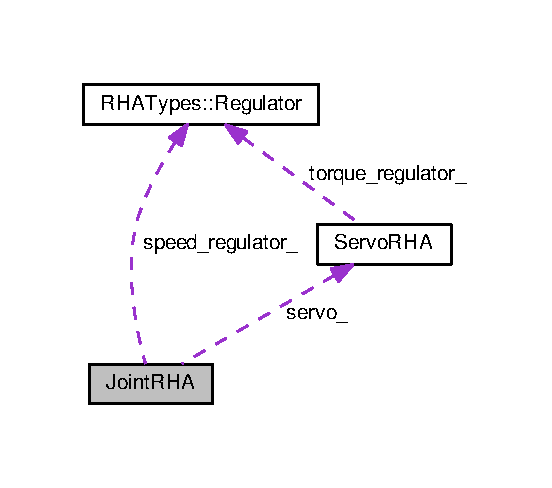
\includegraphics[width=265pt]{classJointRHA__coll__graph}
\end{center}
\end{figure}
\subsection*{Public Member Functions}
\begin{DoxyCompactItemize}
\item 
void {\bfseries print\+Check\+Var} ()\hypertarget{classJointRHA_a21a6d1e5b1eb7844e62fdfa1d1941701}{}\label{classJointRHA_a21a6d1e5b1eb7844e62fdfa1d1941701}

\item 
\hyperlink{classJointRHA_a27538101f833541965c24023a167f709}{Joint\+R\+HA} (uint8\+\_\+t \+\_\+servo\+\_\+id, uint8\+\_\+t \+\_\+up\+\_\+direction, uint8\+\_\+t \+\_\+potentiometer=N\+O\+\_\+\+P\+O\+T\+E\+N\+T\+I\+O\+M\+E\+T\+ER)
\begin{DoxyCompactList}\small\item\em Cunstructor of \hyperlink{classJointRHA}{Joint\+R\+HA} class. \end{DoxyCompactList}\item 
\hyperlink{classJointRHA_a9e54cc4dde103847c9d17f329302a981}{$\sim$\+Joint\+R\+HA} ()\hypertarget{classJointRHA_a9e54cc4dde103847c9d17f329302a981}{}\label{classJointRHA_a9e54cc4dde103847c9d17f329302a981}

\begin{DoxyCompactList}\small\item\em $\sim$\+Joint\+R\+HA destructor of \hyperlink{classJointRHA}{Joint\+R\+HA} class. \end{DoxyCompactList}\item 
void \hyperlink{classJointRHA_a399fcac49d1c527cae46df726c71b5dd}{init} (uint8\+\_\+t \+\_\+servo\+\_\+id, uint8\+\_\+t \+\_\+up\+\_\+direction, float \+\_\+zero\+\_\+compensation=0, uint8\+\_\+t \+\_\+potentiometer=N\+O\+\_\+\+P\+O\+T\+E\+N\+T\+I\+O\+M\+E\+T\+ER)
\begin{DoxyCompactList}\small\item\em Initialization for \hyperlink{classJointRHA}{Joint\+R\+HA} default constructor. \end{DoxyCompactList}\item 
void \hyperlink{classJointRHA_aa3d76b4209929ff800438e5c735697b5}{set\+Pot\+Relation} (float \+\_\+relation=1)
\item 
void {\bfseries init\+Pot\+Measurment} (uint32\+\_\+t \+\_\+pot\+\_\+min\+\_\+value, uint32\+\_\+t \+\_\+pot\+\_\+max\+\_\+value, uint8\+\_\+t \+\_\+angle\+\_\+min\+\_\+value, uint8\+\_\+t \+\_\+angle\+\_\+max\+\_\+value)\hypertarget{classJointRHA_ab2f7b710e7d609c87376b8ed0ef11f42}{}\label{classJointRHA_ab2f7b710e7d609c87376b8ed0ef11f42}

\item 
uint8\+\_\+t {\bfseries set\+Speed\+Goal} (\hyperlink{structRHATypes_1_1SpeedGoal}{R\+H\+A\+Types\+::\+Speed\+Goal} \+\_\+goal)\hypertarget{classJointRHA_a5caf9ac1dd4f9d97917168975af4d3fc}{}\label{classJointRHA_a5caf9ac1dd4f9d97917168975af4d3fc}

\item 
void \hyperlink{classJointRHA_a35e934c28ecaf6870c40ceda272f2391}{update\+Position} ()
\begin{DoxyCompactList}\small\item\em Updates position reading from potentiometer if there is a pot to read (not 255). Updates joint angle position  \hyperlink{classJointRHA_a35e934c28ecaf6870c40ceda272f2391}{Joint\+R\+H\+A\+::update\+Position}. \end{DoxyCompactList}\item 
void \hyperlink{classJointRHA_a47b3cdcdd16e52f60dbcfe3aa52ef540}{update\+Info} (uint8\+\_\+t $\ast$\+\_\+data, uint16\+\_\+t \+\_\+error)
\begin{DoxyCompactList}\small\item\em Updates all the information of servo object information and position feedback of joint to use it in next control iteration (in control loop)  \hyperlink{classJointRHA_a47b3cdcdd16e52f60dbcfe3aa52ef540}{Joint\+R\+H\+A\+::update\+Info}. \end{DoxyCompactList}\item 
void \hyperlink{classJointRHA_a4de486ebe656609fdc0fe7281a69c6eb}{set\+Position\+Goal} (int \+\_\+position)
\begin{DoxyCompactList}\small\item\em Sets a goal position for this joint  set\+Position\+Goal. \end{DoxyCompactList}\item 
void \hyperlink{classJointRHA_a46047d4c042cb9963c9cec7809d02c64}{pos\+Error} ()\hypertarget{classJointRHA_a46047d4c042cb9963c9cec7809d02c64}{}\label{classJointRHA_a46047d4c042cb9963c9cec7809d02c64}

\begin{DoxyCompactList}\small\item\em Calculates error to send to servo regulator. \end{DoxyCompactList}\item 
void \hyperlink{classJointRHA_a8b828c0ac7b125f0ba87d5d76c1c6644}{calculate\+Speed} (float \+\_\+error=0, float \+\_\+derror=0, float \+\_\+ierror=0)
\begin{DoxyCompactList}\small\item\em calculates speed from pos error using regulator. Params are by default 0, it is only used with params for testing pourposes  Joint\+R\+H\+A\+::calculate\+Torque \end{DoxyCompactList}\item 
void \hyperlink{classJointRHA_a83d6397ce8495fcb6aa6c9c787029cb8}{update\+Servo\+Speed\+Goal} ()\hypertarget{classJointRHA_a83d6397ce8495fcb6aa6c9c787029cb8}{}\label{classJointRHA_a83d6397ce8495fcb6aa6c9c787029cb8}

\begin{DoxyCompactList}\small\item\em Updates \hyperlink{classServoRHA}{Servo\+R\+HA} speed goal  \hyperlink{classJointRHA_a83d6397ce8495fcb6aa6c9c787029cb8}{Joint\+R\+H\+A\+::update\+Servo\+Speed\+Goal}. \end{DoxyCompactList}\item 
bool \hyperlink{classJointRHA_a456581be8bd7faa805e8d5d3ee39b38e}{check\+Security} ()
\begin{DoxyCompactList}\small\item\em checks that everithing goes as espected. If not it stops the servo  check\+Security \end{DoxyCompactList}\item 
bool \hyperlink{classJointRHA_af2624db0cab2521e52839e3304aa414d}{reached\+Goal\+Position} ()
\begin{DoxyCompactList}\small\item\em returns true if goal position is reached  \hyperlink{classJointRHA_af2624db0cab2521e52839e3304aa414d}{Joint\+R\+H\+A\+::reached\+Goal\+Position} \end{DoxyCompactList}\item 
float {\bfseries get\+Position} ()\hypertarget{classJointRHA_a520b57b3253406d8de4a93d7469b6033}{}\label{classJointRHA_a520b57b3253406d8de4a93d7469b6033}

\item 
float {\bfseries get\+Goal\+Speed} ()\hypertarget{classJointRHA_aec35bbee89ccc729d8120f3321ae7271}{}\label{classJointRHA_aec35bbee89ccc729d8120f3321ae7271}

\item 
int {\bfseries get\+Pos\+Target} ()\hypertarget{classJointRHA_ad43899febb44ecb4b96424d694b7f273}{}\label{classJointRHA_ad43899febb44ecb4b96424d694b7f273}

\item 
float {\bfseries get\+Error} ()\hypertarget{classJointRHA_ad6747315f3bd4bf5152658d2b6f142f1}{}\label{classJointRHA_ad6747315f3bd4bf5152658d2b6f142f1}

\item 
float {\bfseries get\+D\+Error} ()\hypertarget{classJointRHA_a4d0fdf0043ba63ca8ecca7f9ad391343}{}\label{classJointRHA_a4d0fdf0043ba63ca8ecca7f9ad391343}

\item 
float {\bfseries get\+I\+Error} ()\hypertarget{classJointRHA_a7d2bfb6a14f255ba66bedfba6dda3272}{}\label{classJointRHA_a7d2bfb6a14f255ba66bedfba6dda3272}

\item 
int {\bfseries get\+Analog\+Read\+Pot} ()\hypertarget{classJointRHA_a8317f8455c327eb85b547835125aaacf}{}\label{classJointRHA_a8317f8455c327eb85b547835125aaacf}

\item 
int {\bfseries get\+Potentiometer\+Pin} ()\hypertarget{classJointRHA_ae1a1cd062b222347eafc35ba507054f2}{}\label{classJointRHA_ae1a1cd062b222347eafc35ba507054f2}

\end{DoxyCompactItemize}
\subsection*{Public Attributes}
\begin{DoxyCompactItemize}
\item 
\hyperlink{classRHATypes_1_1Regulator}{R\+H\+A\+Types\+::\+Regulator} {\bfseries speed\+\_\+regulator\+\_\+}\hypertarget{classJointRHA_aa99d8abe21cce0cb10f825224be2dcad}{}\label{classJointRHA_aa99d8abe21cce0cb10f825224be2dcad}

\item 
\hyperlink{classServoRHA}{Servo\+R\+HA} {\bfseries servo\+\_\+}\hypertarget{classJointRHA_a9908ffa793e380e6382a5f0c3afb758d}{}\label{classJointRHA_a9908ffa793e380e6382a5f0c3afb758d}

\end{DoxyCompactItemize}


\subsection{Constructor \& Destructor Documentation}
\index{Joint\+R\+HA@{Joint\+R\+HA}!Joint\+R\+HA@{Joint\+R\+HA}}
\index{Joint\+R\+HA@{Joint\+R\+HA}!Joint\+R\+HA@{Joint\+R\+HA}}
\subsubsection[{\texorpdfstring{Joint\+R\+H\+A(uint8\+\_\+t \+\_\+servo\+\_\+id, uint8\+\_\+t \+\_\+up\+\_\+direction, uint8\+\_\+t \+\_\+potentiometer=\+N\+O\+\_\+\+P\+O\+T\+E\+N\+T\+I\+O\+M\+E\+T\+E\+R)}{JointRHA(uint8_t _servo_id, uint8_t _up_direction, uint8_t _potentiometer=NO_POTENTIOMETER)}}]{\setlength{\rightskip}{0pt plus 5cm}Joint\+R\+H\+A\+::\+Joint\+R\+HA (
\begin{DoxyParamCaption}
\item[{uint8\+\_\+t}]{\+\_\+servo\+\_\+id, }
\item[{uint8\+\_\+t}]{\+\_\+up\+\_\+direction, }
\item[{uint8\+\_\+t}]{\+\_\+potentiometer = {\ttfamily NO\+\_\+POTENTIOMETER}}
\end{DoxyParamCaption}
)}\hypertarget{classJointRHA_a27538101f833541965c24023a167f709}{}\label{classJointRHA_a27538101f833541965c24023a167f709}


Cunstructor of \hyperlink{classJointRHA}{Joint\+R\+HA} class. 


\begin{DoxyParams}{Parameters}
{\em \{uint8\+\_\+t\}} & servo\+\_\+id servo id controlled by this joint \\
\hline
{\em \{uint8\+\_\+t\}} & up\+\_\+direction direction in which the servo has to move (CW or C\+CW) so the joint moves up. \\
\hline
{\em \{uint8\+\_\+t\}} & potentiometer pin in which the potentiometer for this joint is connected. If there is no realim for this joint value will be 255 \\
\hline
\end{DoxyParams}


\subsection{Member Function Documentation}
\index{Joint\+R\+HA@{Joint\+R\+HA}!calculate\+Speed@{calculate\+Speed}}
\index{calculate\+Speed@{calculate\+Speed}!Joint\+R\+HA@{Joint\+R\+HA}}
\subsubsection[{\texorpdfstring{calculate\+Speed(float \+\_\+error=0, float \+\_\+derror=0, float \+\_\+ierror=0)}{calculateSpeed(float _error=0, float _derror=0, float _ierror=0)}}]{\setlength{\rightskip}{0pt plus 5cm}void Joint\+R\+H\+A\+::calculate\+Speed (
\begin{DoxyParamCaption}
\item[{float}]{\+\_\+error = {\ttfamily 0}, }
\item[{float}]{\+\_\+derror = {\ttfamily 0}, }
\item[{float}]{\+\_\+ierror = {\ttfamily 0}}
\end{DoxyParamCaption}
)}\hypertarget{classJointRHA_a8b828c0ac7b125f0ba87d5d76c1c6644}{}\label{classJointRHA_a8b828c0ac7b125f0ba87d5d76c1c6644}


calculates speed from pos error using regulator. Params are by default 0, it is only used with params for testing pourposes  Joint\+R\+H\+A\+::calculate\+Torque 


\begin{DoxyParams}{Parameters}
{\em error} & pos error \\
\hline
{\em derror} & derivative of pos error \\
\hline
{\em ierror} & integral of pos error \\
\hline
\end{DoxyParams}
\index{Joint\+R\+HA@{Joint\+R\+HA}!check\+Security@{check\+Security}}
\index{check\+Security@{check\+Security}!Joint\+R\+HA@{Joint\+R\+HA}}
\subsubsection[{\texorpdfstring{check\+Security()}{checkSecurity()}}]{\setlength{\rightskip}{0pt plus 5cm}bool Joint\+R\+H\+A\+::check\+Security (
\begin{DoxyParamCaption}
{}
\end{DoxyParamCaption}
)}\hypertarget{classJointRHA_a456581be8bd7faa805e8d5d3ee39b38e}{}\label{classJointRHA_a456581be8bd7faa805e8d5d3ee39b38e}


checks that everithing goes as espected. If not it stops the servo  check\+Security 

\begin{DoxyReturn}{Returns}
Returns true when theres no problem, false otherwise 
\end{DoxyReturn}
\index{Joint\+R\+HA@{Joint\+R\+HA}!init@{init}}
\index{init@{init}!Joint\+R\+HA@{Joint\+R\+HA}}
\subsubsection[{\texorpdfstring{init(uint8\+\_\+t \+\_\+servo\+\_\+id, uint8\+\_\+t \+\_\+up\+\_\+direction, float \+\_\+zero\+\_\+compensation=0, uint8\+\_\+t \+\_\+potentiometer=\+N\+O\+\_\+\+P\+O\+T\+E\+N\+T\+I\+O\+M\+E\+T\+E\+R)}{init(uint8_t _servo_id, uint8_t _up_direction, float _zero_compensation=0, uint8_t _potentiometer=NO_POTENTIOMETER)}}]{\setlength{\rightskip}{0pt plus 5cm}void Joint\+R\+H\+A\+::init (
\begin{DoxyParamCaption}
\item[{uint8\+\_\+t}]{\+\_\+servo\+\_\+id, }
\item[{uint8\+\_\+t}]{\+\_\+up\+\_\+direction, }
\item[{float}]{\+\_\+zero\+\_\+compensation = {\ttfamily 0}, }
\item[{uint8\+\_\+t}]{\+\_\+potentiometer = {\ttfamily NO\+\_\+POTENTIOMETER}}
\end{DoxyParamCaption}
)}\hypertarget{classJointRHA_a399fcac49d1c527cae46df726c71b5dd}{}\label{classJointRHA_a399fcac49d1c527cae46df726c71b5dd}


Initialization for \hyperlink{classJointRHA}{Joint\+R\+HA} default constructor. 


\begin{DoxyParams}{Parameters}
{\em \{uint8\+\_\+t\}} & servo\+\_\+id servo id controlled by this joint \\
\hline
{\em \{uint8\+\_\+t\}} & up\+\_\+direction direction in which the servo has to move (CW or C\+CW) so the joint moves up. \\
\hline
{\em \{uint8\+\_\+t\}} & potentiometer pin in which the potentiometer for this joint is connected. If there is no realim for this joint value will be 255 \\
\hline
\end{DoxyParams}
\index{Joint\+R\+HA@{Joint\+R\+HA}!reached\+Goal\+Position@{reached\+Goal\+Position}}
\index{reached\+Goal\+Position@{reached\+Goal\+Position}!Joint\+R\+HA@{Joint\+R\+HA}}
\subsubsection[{\texorpdfstring{reached\+Goal\+Position()}{reachedGoalPosition()}}]{\setlength{\rightskip}{0pt plus 5cm}bool Joint\+R\+H\+A\+::reached\+Goal\+Position (
\begin{DoxyParamCaption}
{}
\end{DoxyParamCaption}
)}\hypertarget{classJointRHA_af2624db0cab2521e52839e3304aa414d}{}\label{classJointRHA_af2624db0cab2521e52839e3304aa414d}


returns true if goal position is reached  \hyperlink{classJointRHA_af2624db0cab2521e52839e3304aa414d}{Joint\+R\+H\+A\+::reached\+Goal\+Position} 

\begin{DoxyReturn}{Returns}
\mbox{[}description\mbox{]} 
\end{DoxyReturn}
\index{Joint\+R\+HA@{Joint\+R\+HA}!set\+Position\+Goal@{set\+Position\+Goal}}
\index{set\+Position\+Goal@{set\+Position\+Goal}!Joint\+R\+HA@{Joint\+R\+HA}}
\subsubsection[{\texorpdfstring{set\+Position\+Goal(int \+\_\+position)}{setPositionGoal(int _position)}}]{\setlength{\rightskip}{0pt plus 5cm}void Joint\+R\+H\+A\+::set\+Position\+Goal (
\begin{DoxyParamCaption}
\item[{int}]{\+\_\+position}
\end{DoxyParamCaption}
)}\hypertarget{classJointRHA_a4de486ebe656609fdc0fe7281a69c6eb}{}\label{classJointRHA_a4de486ebe656609fdc0fe7281a69c6eb}


Sets a goal position for this joint  set\+Position\+Goal. 


\begin{DoxyParams}{Parameters}
{\em position} & position to go \\
\hline
\end{DoxyParams}
\index{Joint\+R\+HA@{Joint\+R\+HA}!set\+Pot\+Relation@{set\+Pot\+Relation}}
\index{set\+Pot\+Relation@{set\+Pot\+Relation}!Joint\+R\+HA@{Joint\+R\+HA}}
\subsubsection[{\texorpdfstring{set\+Pot\+Relation(float \+\_\+relation=1)}{setPotRelation(float _relation=1)}}]{\setlength{\rightskip}{0pt plus 5cm}void Joint\+R\+H\+A\+::set\+Pot\+Relation (
\begin{DoxyParamCaption}
\item[{float}]{\+\_\+relation = {\ttfamily 1}}
\end{DoxyParamCaption}
)}\hypertarget{classJointRHA_aa3d76b4209929ff800438e5c735697b5}{}\label{classJointRHA_aa3d76b4209929ff800438e5c735697b5}
Sets the relation between the potentiometer angle (in grads) and the joint angle  \hyperlink{classJointRHA_aa3d76b4209929ff800438e5c735697b5}{Joint\+R\+H\+A\+::set\+Pot\+Relation} 
\begin{DoxyParams}{Parameters}
{\em \+\_\+relation} & relation between measures. diameter of pot gear / diameter of bar gear \\
\hline
\end{DoxyParams}
\index{Joint\+R\+HA@{Joint\+R\+HA}!update\+Info@{update\+Info}}
\index{update\+Info@{update\+Info}!Joint\+R\+HA@{Joint\+R\+HA}}
\subsubsection[{\texorpdfstring{update\+Info(uint8\+\_\+t $\ast$\+\_\+data, uint16\+\_\+t \+\_\+error)}{updateInfo(uint8_t *_data, uint16_t _error)}}]{\setlength{\rightskip}{0pt plus 5cm}void Joint\+R\+H\+A\+::update\+Info (
\begin{DoxyParamCaption}
\item[{uint8\+\_\+t $\ast$}]{\+\_\+data, }
\item[{uint16\+\_\+t}]{\+\_\+error}
\end{DoxyParamCaption}
)}\hypertarget{classJointRHA_a47b3cdcdd16e52f60dbcfe3aa52ef540}{}\label{classJointRHA_a47b3cdcdd16e52f60dbcfe3aa52ef540}


Updates all the information of servo object information and position feedback of joint to use it in next control iteration (in control loop)  \hyperlink{classJointRHA_a47b3cdcdd16e52f60dbcfe3aa52ef540}{Joint\+R\+H\+A\+::update\+Info}. 


\begin{DoxyParams}{Parameters}
{\em \{uint8\+\_\+t} & $\ast$\} data data with servo information to pass to it \\
\hline
{\em \{uint16\+\_\+t} & $\ast$\} error error in communication with servo \\
\hline
\end{DoxyParams}
\index{Joint\+R\+HA@{Joint\+R\+HA}!update\+Position@{update\+Position}}
\index{update\+Position@{update\+Position}!Joint\+R\+HA@{Joint\+R\+HA}}
\subsubsection[{\texorpdfstring{update\+Position()}{updatePosition()}}]{\setlength{\rightskip}{0pt plus 5cm}void Joint\+R\+H\+A\+::update\+Position (
\begin{DoxyParamCaption}
{}
\end{DoxyParamCaption}
)}\hypertarget{classJointRHA_a35e934c28ecaf6870c40ceda272f2391}{}\label{classJointRHA_a35e934c28ecaf6870c40ceda272f2391}


Updates position reading from potentiometer if there is a pot to read (not 255). Updates joint angle position  \hyperlink{classJointRHA_a35e934c28ecaf6870c40ceda272f2391}{Joint\+R\+H\+A\+::update\+Position}. 

\begin{DoxyReturn}{Returns}
returns position value in joint reference 
\end{DoxyReturn}


The documentation for this class was generated from the following files\+:\begin{DoxyCompactItemize}
\item 
lib/joint\+\_\+rha/\hyperlink{joint__rha_8h}{joint\+\_\+rha.\+h}\item 
lib/joint\+\_\+rha/\hyperlink{joint__rha_8cpp}{joint\+\_\+rha.\+cpp}\end{DoxyCompactItemize}

\hypertarget{classServoRHA}{}\section{Servo\+R\+HA Class Reference}
\label{classServoRHA}\index{Servo\+R\+HA@{Servo\+R\+HA}}


Collaboration diagram for Servo\+R\+HA\+:
\nopagebreak
\begin{figure}[H]
\begin{center}
\leavevmode
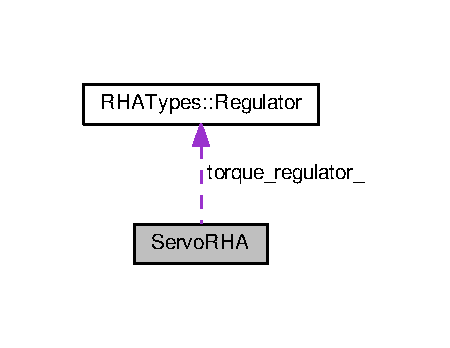
\includegraphics[width=216pt]{classServoRHA__coll__graph}
\end{center}
\end{figure}
\subsection*{Public Member Functions}
\begin{DoxyCompactItemize}
\item 
void {\bfseries print\+Check\+Var} ()\hypertarget{classServoRHA_a576063af699490cd5adb2fa212c8f876}{}\label{classServoRHA_a576063af699490cd5adb2fa212c8f876}

\item 
\hyperlink{classServoRHA_a5206bd5b3e7ecfcc142a1ca15d2a5215}{Servo\+R\+HA} (uint8\+\_\+t \+\_\+servo\+\_\+id)
\begin{DoxyCompactList}\small\item\em Constructor of \hyperlink{classServoRHA}{Servo\+R\+HA} class. \end{DoxyCompactList}\item 
void \hyperlink{classServoRHA_ac2c38ebe6cbd04da613d97e19ed5e257}{init} (uint8\+\_\+t \+\_\+servo\+\_\+id)
\begin{DoxyCompactList}\small\item\em Handles the inicialization of all \hyperlink{classServoRHA}{Servo\+R\+HA} internal parameters when default constructor is used. \end{DoxyCompactList}\item 
void {\bfseries init} ()\hypertarget{classServoRHA_abd64398a4d18799952561bd7a5ded082}{}\label{classServoRHA_abd64398a4d18799952561bd7a5ded082}

\item 
void \hyperlink{classServoRHA_a43b5aa2533b9b1c111ed3b39ac64e894}{update\+Info} (uint8\+\_\+t $\ast$\+\_\+data, uint16\+\_\+t \+\_\+error)
\begin{DoxyCompactList}\small\item\em Asks the servo for all the information to be updated by class servo.  \hyperlink{classServoRHA_a43b5aa2533b9b1c111ed3b39ac64e894}{Servo\+R\+H\+A\+::update\+Info}. \end{DoxyCompactList}\item 
void \hyperlink{classServoRHA_afefa8eadfa7e5e8d001141860fceb0ad}{add\+Return\+Option\+To\+Packet} (uint8\+\_\+t $\ast$\+\_\+buffer, uint8\+\_\+t \+\_\+option)
\begin{DoxyCompactList}\small\item\em Saves in buffer the package return level of servo (error information for each command sent)  \hyperlink{classServoRHA_afefa8eadfa7e5e8d001141860fceb0ad}{Servo\+R\+H\+A\+::add\+Return\+Option\+To\+Packet}. \end{DoxyCompactList}\item 
void \hyperlink{classServoRHA_a57d3a8473a7231b1107d0a69f326dff0}{add\+Upadte\+Info\+To\+Packet} (uint8\+\_\+t $\ast$\+\_\+buffer)
\begin{DoxyCompactList}\small\item\em adds to buffer packet with the uptade info command  \hyperlink{classServoRHA_a57d3a8473a7231b1107d0a69f326dff0}{Servo\+R\+H\+A\+::add\+Upadte\+Info\+To\+Packet} \end{DoxyCompactList}\item 
bool \hyperlink{classServoRHA_a9863a42851b9337cff6b9264cbd457b1}{add\+Torque\+To\+Packet} (uint8\+\_\+t $\ast$\+\_\+buffer)
\begin{DoxyCompactList}\small\item\em Adds this servo torque command to a buffer with his own information. This function is used to send just one packet for all servos instead of each sending their respective information  \hyperlink{classServoRHA_a9863a42851b9337cff6b9264cbd457b1}{Servo\+R\+H\+A\+::add\+Torque\+To\+Packet}. \end{DoxyCompactList}\item 
void \hyperlink{classServoRHA_a80acc3b604abbd21cc4de67127fe34e2}{set\+Torque\+On\+Of\+To\+Packet} (uint8\+\_\+t $\ast$\+\_\+buffer, uint8\+\_\+t \+\_\+on\+Off)
\begin{DoxyCompactList}\small\item\em Adds to buffer information about the torque option (on or off)  \hyperlink{classServoRHA_a80acc3b604abbd21cc4de67127fe34e2}{Servo\+R\+H\+A\+::set\+Torque\+On\+Of\+To\+Packet}. \end{DoxyCompactList}\item 
void \hyperlink{classServoRHA_af7b04ba94b6bc8c2826eb124d220be90}{set\+Wheel\+Mode\+To\+Packet} (uint8\+\_\+t $\ast$\+\_\+buffer)
\begin{DoxyCompactList}\small\item\em Adds to buffer information to set wheel mode for servo  \hyperlink{classServoRHA_af7b04ba94b6bc8c2826eb124d220be90}{Servo\+R\+H\+A\+::set\+Wheel\+Mode\+To\+Packet}. \end{DoxyCompactList}\item 
void \hyperlink{classServoRHA_aae6bc579a9fe9fa4539fa1634bc24682}{exit\+Wheel\+Mode\+To\+Packet} (uint8\+\_\+t $\ast$\+\_\+buffer)
\begin{DoxyCompactList}\small\item\em Adds to buffer information to exit wheel mode for servo  \hyperlink{classServoRHA_aae6bc579a9fe9fa4539fa1634bc24682}{Servo\+R\+H\+A\+::exit\+Wheel\+Mode\+To\+Packet}. \end{DoxyCompactList}\item 
void \hyperlink{classServoRHA_ab496955f29decba4cc13de528344cd5e}{wheel\+Mode\+To\+Packet} (uint8\+\_\+t $\ast$\+\_\+buffer, uint16\+\_\+t \+\_\+\+C\+W\+\_\+angle, uint16\+\_\+t \+\_\+\+C\+C\+W\+\_\+angle)
\begin{DoxyCompactList}\small\item\em Adds to buffer information to set/exit wheel mode for servo. Common function for exit and set functions. \end{DoxyCompactList}\item 
void \hyperlink{classServoRHA_a7f186059f8e620f183b0eca943e9edfa}{add\+To\+Packet} (uint8\+\_\+t $\ast$\+\_\+buffer, uint8\+\_\+t $\ast$\+\_\+packet, uint8\+\_\+t \+\_\+packet\+\_\+len)
\begin{DoxyCompactList}\small\item\em add\+To\+Packet adds this servo to a buffer with his own information (id, goal, etc). This function is used to send just one packet for all servos instead of each sending their respective information \end{DoxyCompactList}\item 
void \hyperlink{classServoRHA_ae3b7cc86e70cea8c0cebcc40d9253569}{ping\+To\+Packet} (uint8\+\_\+t $\ast$\+\_\+buffer)
\begin{DoxyCompactList}\small\item\em Arranges data array to ping action  \hyperlink{classServoRHA_ae3b7cc86e70cea8c0cebcc40d9253569}{Servo\+R\+H\+A\+::ping\+To\+Packet}. \end{DoxyCompactList}\item 
bool \hyperlink{classServoRHA_ac44b27d1ebc80a20d02be44c9b9fe522}{check\+Security} ()
\begin{DoxyCompactList}\small\item\em checks that everithing goes as espected. If not it stops the servo  check\+Security \end{DoxyCompactList}\item 
uint8\+\_\+t \hyperlink{classServoRHA_a90c067d9d37dba8d85aad7faacf5ac7d}{set\+Speed\+Goal} (\hyperlink{structRHATypes_1_1SpeedGoal}{R\+H\+A\+Types\+::\+Speed\+Goal} \+\_\+goal)
\begin{DoxyCompactList}\small\item\em Sets speed goal to achieve with speed slope. \end{DoxyCompactList}\item 
void \hyperlink{classServoRHA_a51a002767a91a7e4c2a8edc9ce8ab0df}{speed\+Error} ()\hypertarget{classServoRHA_a51a002767a91a7e4c2a8edc9ce8ab0df}{}\label{classServoRHA_a51a002767a91a7e4c2a8edc9ce8ab0df}

\begin{DoxyCompactList}\small\item\em Calculates error to send to servo regulator  \hyperlink{classServoRHA_a51a002767a91a7e4c2a8edc9ce8ab0df}{Servo\+R\+H\+A\+::speed\+Error}. \end{DoxyCompactList}\item 
void \hyperlink{classServoRHA_afc5b8b9030190f3165840809faa74d9b}{calculate\+Torque} (float \+\_\+error=0, float \+\_\+derror=0, float \+\_\+ierror=0)
\begin{DoxyCompactList}\small\item\em calculates torque from speed error using regulator. Params are by default 0, it is only used with params for testing pourposes  \hyperlink{classServoRHA_afc5b8b9030190f3165840809faa74d9b}{Servo\+R\+H\+A\+::calculate\+Torque} \end{DoxyCompactList}\item 
void \hyperlink{classServoRHA_ad92cdbe72bb85e809c8cd60ad6701ac9}{set\+Torque\+Limit\+To\+Packet} (uint8\+\_\+t $\ast$\+\_\+buffer, uint16\+\_\+t \+\_\+torque\+\_\+limit)
\begin{DoxyCompactList}\small\item\em Arranges data packet with torque limit  \hyperlink{classServoRHA_ad92cdbe72bb85e809c8cd60ad6701ac9}{Servo\+R\+H\+A\+::set\+Torque\+Limit\+To\+Packet}. \end{DoxyCompactList}\item 
void \hyperlink{classServoRHA_ab2d5a2e9c4d2cbc0bd6e30530b938401}{set\+Wheel\+Speed\+To\+Packet} (uint8\+\_\+t $\ast$\+\_\+buffer, uint16\+\_\+t \+\_\+torque\+\_\+limit, uint8\+\_\+t \+\_\+direction)
\begin{DoxyCompactList}\small\item\em Makes packet with speed goal with set direction  \hyperlink{classServoRHA_ab2d5a2e9c4d2cbc0bd6e30530b938401}{Servo\+R\+H\+A\+::set\+Wheel\+Speed\+To\+Packet}. \end{DoxyCompactList}\item 
virtual uint8\+\_\+t {\bfseries get\+ID} ()\hypertarget{classServoRHA_a5454c2a13b6656a590b7802e88cd1fbb}{}\label{classServoRHA_a5454c2a13b6656a590b7802e88cd1fbb}

\item 
virtual float {\bfseries get\+Speed} ()\hypertarget{classServoRHA_ab104a08e1fe03fc6afd9c3e3af2ab3de}{}\label{classServoRHA_ab104a08e1fe03fc6afd9c3e3af2ab3de}

\item 
virtual uint16\+\_\+t {\bfseries get\+Speed\+Dir} ()\hypertarget{classServoRHA_aebcd18b6b147109d53362d2f61f1687b}{}\label{classServoRHA_aebcd18b6b147109d53362d2f61f1687b}

\item 
virtual uint16\+\_\+t {\bfseries get\+Position} ()\hypertarget{classServoRHA_aae38bc6f06e2b535d1aa97d430f7a754}{}\label{classServoRHA_aae38bc6f06e2b535d1aa97d430f7a754}

\item 
virtual uint16\+\_\+t {\bfseries get\+Load} ()\hypertarget{classServoRHA_add58df5938ca16e07ec9828964221f1b}{}\label{classServoRHA_add58df5938ca16e07ec9828964221f1b}

\item 
virtual uint16\+\_\+t {\bfseries get\+Load\+Dir} ()\hypertarget{classServoRHA_ad130103b70d1cbf88ac1d5875d5d4fa6}{}\label{classServoRHA_ad130103b70d1cbf88ac1d5875d5d4fa6}

\item 
virtual uint16\+\_\+t {\bfseries get\+Goal\+Torque} ()\hypertarget{classServoRHA_ad0b083475f95aed67615eff37644519e}{}\label{classServoRHA_ad0b083475f95aed67615eff37644519e}

\item 
uint16\+\_\+t {\bfseries get\+Speed\+Target} ()\hypertarget{classServoRHA_a6c205569bd752019eba63948520acb16}{}\label{classServoRHA_a6c205569bd752019eba63948520acb16}

\item 
uint8\+\_\+t {\bfseries get\+Direction\+Target} ()\hypertarget{classServoRHA_af700fe03ccea5bb3400a5541274ac6ca}{}\label{classServoRHA_af700fe03ccea5bb3400a5541274ac6ca}

\item 
float {\bfseries get\+Error} ()\hypertarget{classServoRHA_a8c7d84f89e72ec21756383a35b8c3977}{}\label{classServoRHA_a8c7d84f89e72ec21756383a35b8c3977}

\item 
float {\bfseries get\+D\+Error} ()\hypertarget{classServoRHA_a3abf8faab5d85ad0becf54518170ca9e}{}\label{classServoRHA_a3abf8faab5d85ad0becf54518170ca9e}

\item 
float {\bfseries get\+I\+Error} ()\hypertarget{classServoRHA_a3aec41440a26ae7ecb94655125f4013f}{}\label{classServoRHA_a3aec41440a26ae7ecb94655125f4013f}

\item 
uint16\+\_\+t {\bfseries get\+Speed\+With\+Dir} ()\hypertarget{classServoRHA_a2578a759d6d493b865a5309bb2355ea5}{}\label{classServoRHA_a2578a759d6d493b865a5309bb2355ea5}

\item 
uint16\+\_\+t {\bfseries get\+Torque\+With\+Dir} ()\hypertarget{classServoRHA_afd5ea0a7b70a89e30180df7f1c9874f7}{}\label{classServoRHA_afd5ea0a7b70a89e30180df7f1c9874f7}

\end{DoxyCompactItemize}
\subsection*{Public Attributes}
\begin{DoxyCompactItemize}
\item 
\hyperlink{classRHATypes_1_1Regulator}{R\+H\+A\+Types\+::\+Regulator} {\bfseries torque\+\_\+regulator\+\_\+}\hypertarget{classServoRHA_a77b0313984444f5b1f09ff0ecf10f975}{}\label{classServoRHA_a77b0313984444f5b1f09ff0ecf10f975}

\end{DoxyCompactItemize}
\subsection*{Protected Attributes}
\begin{DoxyCompactItemize}
\item 
uint8\+\_\+t {\bfseries empty\+\_\+var}\hypertarget{classServoRHA_a1eb1f55285b79afb966d7d44f64f2aad}{}\label{classServoRHA_a1eb1f55285b79afb966d7d44f64f2aad}

\item 
uint8\+\_\+t {\bfseries empty\+\_\+var\+\_\+2}\hypertarget{classServoRHA_a0e351736018b2bc064d03b51008a0b34}{}\label{classServoRHA_a0e351736018b2bc064d03b51008a0b34}

\item 
volatile uint8\+\_\+t {\bfseries servo\+\_\+id\+\_\+}\hypertarget{classServoRHA_a0a61bbe5f4fd99d39983eb18c7b72823}{}\label{classServoRHA_a0a61bbe5f4fd99d39983eb18c7b72823}

\item 
uint16\+\_\+t {\bfseries speed\+\_\+dir\+\_\+}\hypertarget{classServoRHA_af7c1f52f2b9e8967b9c0b9b65096df48}{}\label{classServoRHA_af7c1f52f2b9e8967b9c0b9b65096df48}

\item 
uint16\+\_\+t {\bfseries position\+\_\+}\hypertarget{classServoRHA_a805b5065a85efc7d94934c0153558c53}{}\label{classServoRHA_a805b5065a85efc7d94934c0153558c53}

\item 
uint16\+\_\+t {\bfseries load\+\_\+}\hypertarget{classServoRHA_ab90b1db8354453f69f9d3c8ba5fb9c8e}{}\label{classServoRHA_ab90b1db8354453f69f9d3c8ba5fb9c8e}

\item 
uint16\+\_\+t {\bfseries load\+\_\+dir\+\_\+}\hypertarget{classServoRHA_a3ffd7c50b36f3dd678541b8750fd6034}{}\label{classServoRHA_a3ffd7c50b36f3dd678541b8750fd6034}

\item 
uint16\+\_\+t {\bfseries error\+\_\+comunication\+\_\+}\hypertarget{classServoRHA_a03ac69ae40642aab24fcadd8d1623c1d}{}\label{classServoRHA_a03ac69ae40642aab24fcadd8d1623c1d}

\item 
float {\bfseries speed\+\_\+}\hypertarget{classServoRHA_a155758e5879714b586ba32e553642115}{}\label{classServoRHA_a155758e5879714b586ba32e553642115}

\item 
uint16\+\_\+t {\bfseries goal\+\_\+torque\+\_\+}\hypertarget{classServoRHA_a6a48b430015c516a83ed9a98ce5fdf0d}{}\label{classServoRHA_a6a48b430015c516a83ed9a98ce5fdf0d}

\item 
uint8\+\_\+t {\bfseries direction\+\_\+target\+\_\+}\hypertarget{classServoRHA_abe8af8cb40c296e2968687b88dc33d56}{}\label{classServoRHA_abe8af8cb40c296e2968687b88dc33d56}

\item 
uint16\+\_\+t {\bfseries speed\+\_\+target\+\_\+}\hypertarget{classServoRHA_a3b574e8f04b1dae947150fa30bc43f24}{}\label{classServoRHA_a3b574e8f04b1dae947150fa30bc43f24}

\item 
uint64\+\_\+t {\bfseries time\+\_\+last\+\_\+}\hypertarget{classServoRHA_afd05b28b211b6a979cfd097cdd159fae}{}\label{classServoRHA_afd05b28b211b6a979cfd097cdd159fae}

\item 
uint64\+\_\+t {\bfseries time\+\_\+last\+\_\+error\+\_\+}\hypertarget{classServoRHA_a4706f2f2cdec3ef979e1eeb887021100}{}\label{classServoRHA_a4706f2f2cdec3ef979e1eeb887021100}

\item 
float {\bfseries error\+\_\+}\hypertarget{classServoRHA_a3f7ba11e56f7706614e6759816a0dbae}{}\label{classServoRHA_a3f7ba11e56f7706614e6759816a0dbae}

\item 
float {\bfseries last\+\_\+error\+\_\+}\hypertarget{classServoRHA_ad90c95c35f78052260b94c9912700d2d}{}\label{classServoRHA_ad90c95c35f78052260b94c9912700d2d}

\item 
float {\bfseries derror\+\_\+}\hypertarget{classServoRHA_abc0e8fa612a0aca1e18833b7fc000ba9}{}\label{classServoRHA_abc0e8fa612a0aca1e18833b7fc000ba9}

\item 
float {\bfseries ierror\+\_\+}\hypertarget{classServoRHA_a1d4bcfc7e29e3c8a6c5525fc951cd90a}{}\label{classServoRHA_a1d4bcfc7e29e3c8a6c5525fc951cd90a}

\end{DoxyCompactItemize}


\subsection{Constructor \& Destructor Documentation}
\index{Servo\+R\+HA@{Servo\+R\+HA}!Servo\+R\+HA@{Servo\+R\+HA}}
\index{Servo\+R\+HA@{Servo\+R\+HA}!Servo\+R\+HA@{Servo\+R\+HA}}
\subsubsection[{\texorpdfstring{Servo\+R\+H\+A(uint8\+\_\+t \+\_\+servo\+\_\+id)}{ServoRHA(uint8_t _servo_id)}}]{\setlength{\rightskip}{0pt plus 5cm}Servo\+R\+H\+A\+::\+Servo\+R\+HA (
\begin{DoxyParamCaption}
\item[{uint8\+\_\+t}]{servo\+\_\+id}
\end{DoxyParamCaption}
)\hspace{0.3cm}{\ttfamily [explicit]}}\hypertarget{classServoRHA_a5206bd5b3e7ecfcc142a1ca15d2a5215}{}\label{classServoRHA_a5206bd5b3e7ecfcc142a1ca15d2a5215}


Constructor of \hyperlink{classServoRHA}{Servo\+R\+HA} class. 


\begin{DoxyParams}{Parameters}
{\em \{uint8\+\_\+t\}} & servo\+\_\+id servo id controlled by this object \\
\hline
\end{DoxyParams}


\subsection{Member Function Documentation}
\index{Servo\+R\+HA@{Servo\+R\+HA}!add\+Return\+Option\+To\+Packet@{add\+Return\+Option\+To\+Packet}}
\index{add\+Return\+Option\+To\+Packet@{add\+Return\+Option\+To\+Packet}!Servo\+R\+HA@{Servo\+R\+HA}}
\subsubsection[{\texorpdfstring{add\+Return\+Option\+To\+Packet(uint8\+\_\+t $\ast$\+\_\+buffer, uint8\+\_\+t \+\_\+option)}{addReturnOptionToPacket(uint8_t *_buffer, uint8_t _option)}}]{\setlength{\rightskip}{0pt plus 5cm}void Servo\+R\+H\+A\+::add\+Return\+Option\+To\+Packet (
\begin{DoxyParamCaption}
\item[{uint8\+\_\+t $\ast$}]{\+\_\+buffer, }
\item[{uint8\+\_\+t}]{\+\_\+option}
\end{DoxyParamCaption}
)}\hypertarget{classServoRHA_afefa8eadfa7e5e8d001141860fceb0ad}{}\label{classServoRHA_afefa8eadfa7e5e8d001141860fceb0ad}


Saves in buffer the package return level of servo (error information for each command sent)  \hyperlink{classServoRHA_afefa8eadfa7e5e8d001141860fceb0ad}{Servo\+R\+H\+A\+::add\+Return\+Option\+To\+Packet}. 


\begin{DoxyParams}{Parameters}
{\em \{uint8\+\_\+t$\ast$\}} & buffer array in which add the information \\
\hline
{\em \{uint8\+\_\+t\}} & option R\+E\+T\+U\+R\+N\+\_\+\+P\+A\+C\+K\+E\+T\+\_\+\+A\+LL -\/$>$ servo returns packet for all commands sent; R\+E\+T\+U\+R\+N\+\_\+\+P\+A\+C\+K\+E\+T\+\_\+\+N\+O\+NE -\/$>$ servo never retunrs state packet; R\+E\+T\+U\+R\+N\+\_\+\+P\+A\+C\+K\+E\+T\+\_\+\+R\+E\+A\+D\+\_\+\+I\+N\+S\+T\+R\+U\+C\+T\+I\+O\+NS -\/$>$ servo answer packet state when a R\+E\+AD command is sent (to read position, temperature, etc) \\
\hline
\end{DoxyParams}
\begin{DoxySeeAlso}{See also}
\hyperlink{classServoRHA_a7f186059f8e620f183b0eca943e9edfa}{add\+To\+Packet()} 
\end{DoxySeeAlso}
\index{Servo\+R\+HA@{Servo\+R\+HA}!add\+To\+Packet@{add\+To\+Packet}}
\index{add\+To\+Packet@{add\+To\+Packet}!Servo\+R\+HA@{Servo\+R\+HA}}
\subsubsection[{\texorpdfstring{add\+To\+Packet(uint8\+\_\+t $\ast$\+\_\+buffer, uint8\+\_\+t $\ast$\+\_\+packet, uint8\+\_\+t \+\_\+packet\+\_\+len)}{addToPacket(uint8_t *_buffer, uint8_t *_packet, uint8_t _packet_len)}}]{\setlength{\rightskip}{0pt plus 5cm}void Servo\+R\+H\+A\+::add\+To\+Packet (
\begin{DoxyParamCaption}
\item[{uint8\+\_\+t $\ast$}]{\+\_\+buffer, }
\item[{uint8\+\_\+t $\ast$}]{\+\_\+packet, }
\item[{uint8\+\_\+t}]{\+\_\+packet\+\_\+len}
\end{DoxyParamCaption}
)}\hypertarget{classServoRHA_a7f186059f8e620f183b0eca943e9edfa}{}\label{classServoRHA_a7f186059f8e620f183b0eca943e9edfa}


add\+To\+Packet adds this servo to a buffer with his own information (id, goal, etc). This function is used to send just one packet for all servos instead of each sending their respective information 


\begin{DoxyParams}{Parameters}
{\em \{uint8\+\_\+t} & $\ast$\} buffer is the buffer in which the information will be added (by reference) \\
\hline
{\em \{uint8\+\_\+t} & $\ast$\} packet small packet to add. Note that it can be speed, torque, position... It can be a combination (go to an X position with an Y speed) (by reference) \\
\hline
{\em \{uint8\+\_\+t\}} & packet\+\_\+len length of the small packet to add (uint8\+\_\+ts) \\
\hline
\end{DoxyParams}
\index{Servo\+R\+HA@{Servo\+R\+HA}!add\+Torque\+To\+Packet@{add\+Torque\+To\+Packet}}
\index{add\+Torque\+To\+Packet@{add\+Torque\+To\+Packet}!Servo\+R\+HA@{Servo\+R\+HA}}
\subsubsection[{\texorpdfstring{add\+Torque\+To\+Packet(uint8\+\_\+t $\ast$\+\_\+buffer)}{addTorqueToPacket(uint8_t *_buffer)}}]{\setlength{\rightskip}{0pt plus 5cm}bool Servo\+R\+H\+A\+::add\+Torque\+To\+Packet (
\begin{DoxyParamCaption}
\item[{uint8\+\_\+t $\ast$}]{\+\_\+buffer}
\end{DoxyParamCaption}
)}\hypertarget{classServoRHA_a9863a42851b9337cff6b9264cbd457b1}{}\label{classServoRHA_a9863a42851b9337cff6b9264cbd457b1}


Adds this servo torque command to a buffer with his own information. This function is used to send just one packet for all servos instead of each sending their respective information  \hyperlink{classServoRHA_a9863a42851b9337cff6b9264cbd457b1}{Servo\+R\+H\+A\+::add\+Torque\+To\+Packet}. 


\begin{DoxyParams}{Parameters}
{\em \{uint8\+\_\+t} & $\ast$\} buffer is the buffer in which the information will be added (by reference) \\
\hline
\end{DoxyParams}
\begin{DoxySeeAlso}{See also}
\hyperlink{classServoRHA_a7f186059f8e620f183b0eca943e9edfa}{add\+To\+Packet()} 
\end{DoxySeeAlso}
\index{Servo\+R\+HA@{Servo\+R\+HA}!add\+Upadte\+Info\+To\+Packet@{add\+Upadte\+Info\+To\+Packet}}
\index{add\+Upadte\+Info\+To\+Packet@{add\+Upadte\+Info\+To\+Packet}!Servo\+R\+HA@{Servo\+R\+HA}}
\subsubsection[{\texorpdfstring{add\+Upadte\+Info\+To\+Packet(uint8\+\_\+t $\ast$\+\_\+buffer)}{addUpadteInfoToPacket(uint8_t *_buffer)}}]{\setlength{\rightskip}{0pt plus 5cm}void Servo\+R\+H\+A\+::add\+Upadte\+Info\+To\+Packet (
\begin{DoxyParamCaption}
\item[{uint8\+\_\+t $\ast$}]{\+\_\+buffer}
\end{DoxyParamCaption}
)}\hypertarget{classServoRHA_a57d3a8473a7231b1107d0a69f326dff0}{}\label{classServoRHA_a57d3a8473a7231b1107d0a69f326dff0}


adds to buffer packet with the uptade info command  \hyperlink{classServoRHA_a57d3a8473a7231b1107d0a69f326dff0}{Servo\+R\+H\+A\+::add\+Upadte\+Info\+To\+Packet} 


\begin{DoxyParams}{Parameters}
{\em \{uint8\+\_\+t$\ast$\}} & buffer array in which add the information \\
\hline
\end{DoxyParams}
\index{Servo\+R\+HA@{Servo\+R\+HA}!calculate\+Torque@{calculate\+Torque}}
\index{calculate\+Torque@{calculate\+Torque}!Servo\+R\+HA@{Servo\+R\+HA}}
\subsubsection[{\texorpdfstring{calculate\+Torque(float \+\_\+error=0, float \+\_\+derror=0, float \+\_\+ierror=0)}{calculateTorque(float _error=0, float _derror=0, float _ierror=0)}}]{\setlength{\rightskip}{0pt plus 5cm}void Servo\+R\+H\+A\+::calculate\+Torque (
\begin{DoxyParamCaption}
\item[{float}]{\+\_\+error = {\ttfamily 0}, }
\item[{float}]{\+\_\+derror = {\ttfamily 0}, }
\item[{float}]{\+\_\+ierror = {\ttfamily 0}}
\end{DoxyParamCaption}
)}\hypertarget{classServoRHA_afc5b8b9030190f3165840809faa74d9b}{}\label{classServoRHA_afc5b8b9030190f3165840809faa74d9b}


calculates torque from speed error using regulator. Params are by default 0, it is only used with params for testing pourposes  \hyperlink{classServoRHA_afc5b8b9030190f3165840809faa74d9b}{Servo\+R\+H\+A\+::calculate\+Torque} 


\begin{DoxyParams}{Parameters}
{\em error} & speed error \\
\hline
{\em derror} & derivative of speed error \\
\hline
{\em ierror} & integral of speed error \\
\hline
\end{DoxyParams}
\index{Servo\+R\+HA@{Servo\+R\+HA}!check\+Security@{check\+Security}}
\index{check\+Security@{check\+Security}!Servo\+R\+HA@{Servo\+R\+HA}}
\subsubsection[{\texorpdfstring{check\+Security()}{checkSecurity()}}]{\setlength{\rightskip}{0pt plus 5cm}bool Servo\+R\+H\+A\+::check\+Security (
\begin{DoxyParamCaption}
{}
\end{DoxyParamCaption}
)}\hypertarget{classServoRHA_ac44b27d1ebc80a20d02be44c9b9fe522}{}\label{classServoRHA_ac44b27d1ebc80a20d02be44c9b9fe522}


checks that everithing goes as espected. If not it stops the servo  check\+Security 

\begin{DoxyReturn}{Returns}
Returns true when theres no problem, false otherwise 
\end{DoxyReturn}
\index{Servo\+R\+HA@{Servo\+R\+HA}!exit\+Wheel\+Mode\+To\+Packet@{exit\+Wheel\+Mode\+To\+Packet}}
\index{exit\+Wheel\+Mode\+To\+Packet@{exit\+Wheel\+Mode\+To\+Packet}!Servo\+R\+HA@{Servo\+R\+HA}}
\subsubsection[{\texorpdfstring{exit\+Wheel\+Mode\+To\+Packet(uint8\+\_\+t $\ast$\+\_\+buffer)}{exitWheelModeToPacket(uint8_t *_buffer)}}]{\setlength{\rightskip}{0pt plus 5cm}void Servo\+R\+H\+A\+::exit\+Wheel\+Mode\+To\+Packet (
\begin{DoxyParamCaption}
\item[{uint8\+\_\+t $\ast$}]{\+\_\+buffer}
\end{DoxyParamCaption}
)}\hypertarget{classServoRHA_aae6bc579a9fe9fa4539fa1634bc24682}{}\label{classServoRHA_aae6bc579a9fe9fa4539fa1634bc24682}


Adds to buffer information to exit wheel mode for servo  \hyperlink{classServoRHA_aae6bc579a9fe9fa4539fa1634bc24682}{Servo\+R\+H\+A\+::exit\+Wheel\+Mode\+To\+Packet}. 


\begin{DoxyParams}{Parameters}
{\em buffer} & array in which add the information \\
\hline
\end{DoxyParams}
\begin{DoxySeeAlso}{See also}
\hyperlink{classServoRHA_af7b04ba94b6bc8c2826eb124d220be90}{set\+Wheel\+Mode\+To\+Packet()} 

\hyperlink{classServoRHA_ab496955f29decba4cc13de528344cd5e}{wheel\+Mode\+To\+Packet()} 
\end{DoxySeeAlso}
\index{Servo\+R\+HA@{Servo\+R\+HA}!init@{init}}
\index{init@{init}!Servo\+R\+HA@{Servo\+R\+HA}}
\subsubsection[{\texorpdfstring{init(uint8\+\_\+t \+\_\+servo\+\_\+id)}{init(uint8_t _servo_id)}}]{\setlength{\rightskip}{0pt plus 5cm}void Servo\+R\+H\+A\+::init (
\begin{DoxyParamCaption}
\item[{uint8\+\_\+t}]{\+\_\+servo\+\_\+id}
\end{DoxyParamCaption}
)}\hypertarget{classServoRHA_ac2c38ebe6cbd04da613d97e19ed5e257}{}\label{classServoRHA_ac2c38ebe6cbd04da613d97e19ed5e257}


Handles the inicialization of all \hyperlink{classServoRHA}{Servo\+R\+HA} internal parameters when default constructor is used. 


\begin{DoxyParams}{Parameters}
{\em \{uint8\+\_\+t\}} & servo\+\_\+id servo id controlled by this object \\
\hline
\end{DoxyParams}
\index{Servo\+R\+HA@{Servo\+R\+HA}!ping\+To\+Packet@{ping\+To\+Packet}}
\index{ping\+To\+Packet@{ping\+To\+Packet}!Servo\+R\+HA@{Servo\+R\+HA}}
\subsubsection[{\texorpdfstring{ping\+To\+Packet(uint8\+\_\+t $\ast$\+\_\+buffer)}{pingToPacket(uint8_t *_buffer)}}]{\setlength{\rightskip}{0pt plus 5cm}void Servo\+R\+H\+A\+::ping\+To\+Packet (
\begin{DoxyParamCaption}
\item[{uint8\+\_\+t $\ast$}]{\+\_\+buffer}
\end{DoxyParamCaption}
)}\hypertarget{classServoRHA_ae3b7cc86e70cea8c0cebcc40d9253569}{}\label{classServoRHA_ae3b7cc86e70cea8c0cebcc40d9253569}


Arranges data array to ping action  \hyperlink{classServoRHA_ae3b7cc86e70cea8c0cebcc40d9253569}{Servo\+R\+H\+A\+::ping\+To\+Packet}. 


\begin{DoxyParams}{Parameters}
{\em buffer} & Array in which to store the data \\
\hline
\end{DoxyParams}
\index{Servo\+R\+HA@{Servo\+R\+HA}!set\+Speed\+Goal@{set\+Speed\+Goal}}
\index{set\+Speed\+Goal@{set\+Speed\+Goal}!Servo\+R\+HA@{Servo\+R\+HA}}
\subsubsection[{\texorpdfstring{set\+Speed\+Goal(\+R\+H\+A\+Types\+::\+Speed\+Goal \+\_\+goal)}{setSpeedGoal(RHATypes::SpeedGoal _goal)}}]{\setlength{\rightskip}{0pt plus 5cm}uint8\+\_\+t Servo\+R\+H\+A\+::set\+Speed\+Goal (
\begin{DoxyParamCaption}
\item[{{\bf R\+H\+A\+Types\+::\+Speed\+Goal}}]{\+\_\+goal}
\end{DoxyParamCaption}
)}\hypertarget{classServoRHA_a90c067d9d37dba8d85aad7faacf5ac7d}{}\label{classServoRHA_a90c067d9d37dba8d85aad7faacf5ac7d}


Sets speed goal to achieve with speed slope. 


\begin{DoxyParams}{Parameters}
{\em \{uint16\+\_\+t\}} & speed\+\_\+target speed to achieve \\
\hline
{\em \{uint16\+\_\+t\}} & direction\+\_\+target move CW or C\+CW \\
\hline
\end{DoxyParams}
\index{Servo\+R\+HA@{Servo\+R\+HA}!set\+Torque\+Limit\+To\+Packet@{set\+Torque\+Limit\+To\+Packet}}
\index{set\+Torque\+Limit\+To\+Packet@{set\+Torque\+Limit\+To\+Packet}!Servo\+R\+HA@{Servo\+R\+HA}}
\subsubsection[{\texorpdfstring{set\+Torque\+Limit\+To\+Packet(uint8\+\_\+t $\ast$\+\_\+buffer, uint16\+\_\+t \+\_\+torque\+\_\+limit)}{setTorqueLimitToPacket(uint8_t *_buffer, uint16_t _torque_limit)}}]{\setlength{\rightskip}{0pt plus 5cm}void Servo\+R\+H\+A\+::set\+Torque\+Limit\+To\+Packet (
\begin{DoxyParamCaption}
\item[{uint8\+\_\+t $\ast$}]{\+\_\+buffer, }
\item[{uint16\+\_\+t}]{\+\_\+torque\+\_\+limit}
\end{DoxyParamCaption}
)}\hypertarget{classServoRHA_ad92cdbe72bb85e809c8cd60ad6701ac9}{}\label{classServoRHA_ad92cdbe72bb85e809c8cd60ad6701ac9}


Arranges data packet with torque limit  \hyperlink{classServoRHA_ad92cdbe72bb85e809c8cd60ad6701ac9}{Servo\+R\+H\+A\+::set\+Torque\+Limit\+To\+Packet}. 


\begin{DoxyParams}{Parameters}
{\em buffer} & Array in which to store the data \\
\hline
{\em torque\+\_\+limit} & Torque limit to set \\
\hline
\end{DoxyParams}
\index{Servo\+R\+HA@{Servo\+R\+HA}!set\+Torque\+On\+Of\+To\+Packet@{set\+Torque\+On\+Of\+To\+Packet}}
\index{set\+Torque\+On\+Of\+To\+Packet@{set\+Torque\+On\+Of\+To\+Packet}!Servo\+R\+HA@{Servo\+R\+HA}}
\subsubsection[{\texorpdfstring{set\+Torque\+On\+Of\+To\+Packet(uint8\+\_\+t $\ast$\+\_\+buffer, uint8\+\_\+t \+\_\+on\+Off)}{setTorqueOnOfToPacket(uint8_t *_buffer, uint8_t _onOff)}}]{\setlength{\rightskip}{0pt plus 5cm}void Servo\+R\+H\+A\+::set\+Torque\+On\+Of\+To\+Packet (
\begin{DoxyParamCaption}
\item[{uint8\+\_\+t $\ast$}]{\+\_\+buffer, }
\item[{uint8\+\_\+t}]{\+\_\+on\+Off}
\end{DoxyParamCaption}
)}\hypertarget{classServoRHA_a80acc3b604abbd21cc4de67127fe34e2}{}\label{classServoRHA_a80acc3b604abbd21cc4de67127fe34e2}


Adds to buffer information about the torque option (on or off)  \hyperlink{classServoRHA_a80acc3b604abbd21cc4de67127fe34e2}{Servo\+R\+H\+A\+::set\+Torque\+On\+Of\+To\+Packet}. 


\begin{DoxyParams}{Parameters}
{\em buffer} & array in which add the information \\
\hline
{\em on\+Off} & ON = 1; O\+FF = 0; \\
\hline
\end{DoxyParams}
\index{Servo\+R\+HA@{Servo\+R\+HA}!set\+Wheel\+Mode\+To\+Packet@{set\+Wheel\+Mode\+To\+Packet}}
\index{set\+Wheel\+Mode\+To\+Packet@{set\+Wheel\+Mode\+To\+Packet}!Servo\+R\+HA@{Servo\+R\+HA}}
\subsubsection[{\texorpdfstring{set\+Wheel\+Mode\+To\+Packet(uint8\+\_\+t $\ast$\+\_\+buffer)}{setWheelModeToPacket(uint8_t *_buffer)}}]{\setlength{\rightskip}{0pt plus 5cm}void Servo\+R\+H\+A\+::set\+Wheel\+Mode\+To\+Packet (
\begin{DoxyParamCaption}
\item[{uint8\+\_\+t $\ast$}]{\+\_\+buffer}
\end{DoxyParamCaption}
)}\hypertarget{classServoRHA_af7b04ba94b6bc8c2826eb124d220be90}{}\label{classServoRHA_af7b04ba94b6bc8c2826eb124d220be90}


Adds to buffer information to set wheel mode for servo  \hyperlink{classServoRHA_af7b04ba94b6bc8c2826eb124d220be90}{Servo\+R\+H\+A\+::set\+Wheel\+Mode\+To\+Packet}. 


\begin{DoxyParams}{Parameters}
{\em buffer} & array in which add the information \\
\hline
\end{DoxyParams}
\begin{DoxySeeAlso}{See also}
\hyperlink{classServoRHA_aae6bc579a9fe9fa4539fa1634bc24682}{exit\+Wheel\+Mode\+To\+Packet()} 

\hyperlink{classServoRHA_ab496955f29decba4cc13de528344cd5e}{wheel\+Mode\+To\+Packet()} 
\end{DoxySeeAlso}
\index{Servo\+R\+HA@{Servo\+R\+HA}!set\+Wheel\+Speed\+To\+Packet@{set\+Wheel\+Speed\+To\+Packet}}
\index{set\+Wheel\+Speed\+To\+Packet@{set\+Wheel\+Speed\+To\+Packet}!Servo\+R\+HA@{Servo\+R\+HA}}
\subsubsection[{\texorpdfstring{set\+Wheel\+Speed\+To\+Packet(uint8\+\_\+t $\ast$\+\_\+buffer, uint16\+\_\+t \+\_\+torque\+\_\+limit, uint8\+\_\+t \+\_\+direction)}{setWheelSpeedToPacket(uint8_t *_buffer, uint16_t _torque_limit, uint8_t _direction)}}]{\setlength{\rightskip}{0pt plus 5cm}void Servo\+R\+H\+A\+::set\+Wheel\+Speed\+To\+Packet (
\begin{DoxyParamCaption}
\item[{uint8\+\_\+t $\ast$}]{\+\_\+buffer, }
\item[{uint16\+\_\+t}]{\+\_\+speed, }
\item[{uint8\+\_\+t}]{\+\_\+direction}
\end{DoxyParamCaption}
)}\hypertarget{classServoRHA_ab2d5a2e9c4d2cbc0bd6e30530b938401}{}\label{classServoRHA_ab2d5a2e9c4d2cbc0bd6e30530b938401}


Makes packet with speed goal with set direction  \hyperlink{classServoRHA_ab2d5a2e9c4d2cbc0bd6e30530b938401}{Servo\+R\+H\+A\+::set\+Wheel\+Speed\+To\+Packet}. 


\begin{DoxyParams}{Parameters}
{\em buffer} & Array in which to store the data \\
\hline
{\em speed} & Speed to set \\
\hline
{\em direction} & Direction in which servo will move \\
\hline
\end{DoxyParams}
\index{Servo\+R\+HA@{Servo\+R\+HA}!update\+Info@{update\+Info}}
\index{update\+Info@{update\+Info}!Servo\+R\+HA@{Servo\+R\+HA}}
\subsubsection[{\texorpdfstring{update\+Info(uint8\+\_\+t $\ast$\+\_\+data, uint16\+\_\+t \+\_\+error)}{updateInfo(uint8_t *_data, uint16_t _error)}}]{\setlength{\rightskip}{0pt plus 5cm}void Servo\+R\+H\+A\+::update\+Info (
\begin{DoxyParamCaption}
\item[{uint8\+\_\+t $\ast$}]{\+\_\+data, }
\item[{uint16\+\_\+t}]{\+\_\+error}
\end{DoxyParamCaption}
)}\hypertarget{classServoRHA_a43b5aa2533b9b1c111ed3b39ac64e894}{}\label{classServoRHA_a43b5aa2533b9b1c111ed3b39ac64e894}


Asks the servo for all the information to be updated by class servo.  \hyperlink{classServoRHA_a43b5aa2533b9b1c111ed3b39ac64e894}{Servo\+R\+H\+A\+::update\+Info}. 


\begin{DoxyParams}{Parameters}
{\em \{uint8\+\_\+t} & $\ast$\} data Array containing all the data \\
\hline
{\em \{uint16\+\_\+t\}} & error Error in comunication\\
\hline
\end{DoxyParams}
Reads from register P\+R\+E\+S\+E\+N\+T\+\_\+\+P\+O\+S\+I\+T\+I\+O\+N\+\_\+L (0x24) to M\+O\+V\+I\+NG (0x2E). Position are bits 10 to 0 from register 0x24 and 0x25 Speed are bits 9 to 0 from register 0x26 and 0x27, 10th bit is direction Load are bits 9 to 0 from register 0x28 and 0x29, 10th bit is direction

To avoid spending too much time the following parameter have been commented as they are not used

Voltage is in register 0x2a Temperature is in register 0x2B Action registered (pending from activation) flag is in register 0x2C Moving flag is in register 0x2E \index{Servo\+R\+HA@{Servo\+R\+HA}!wheel\+Mode\+To\+Packet@{wheel\+Mode\+To\+Packet}}
\index{wheel\+Mode\+To\+Packet@{wheel\+Mode\+To\+Packet}!Servo\+R\+HA@{Servo\+R\+HA}}
\subsubsection[{\texorpdfstring{wheel\+Mode\+To\+Packet(uint8\+\_\+t $\ast$\+\_\+buffer, uint16\+\_\+t \+\_\+\+C\+W\+\_\+angle, uint16\+\_\+t \+\_\+\+C\+C\+W\+\_\+angle)}{wheelModeToPacket(uint8_t *_buffer, uint16_t _CW_angle, uint16_t _CCW_angle)}}]{\setlength{\rightskip}{0pt plus 5cm}void Servo\+R\+H\+A\+::wheel\+Mode\+To\+Packet (
\begin{DoxyParamCaption}
\item[{uint8\+\_\+t $\ast$}]{\+\_\+buffer, }
\item[{uint16\+\_\+t}]{\+\_\+\+C\+W\+\_\+angle, }
\item[{uint16\+\_\+t}]{\+\_\+\+C\+C\+W\+\_\+angle}
\end{DoxyParamCaption}
)}\hypertarget{classServoRHA_ab496955f29decba4cc13de528344cd5e}{}\label{classServoRHA_ab496955f29decba4cc13de528344cd5e}


Adds to buffer information to set/exit wheel mode for servo. Common function for exit and set functions. 


\begin{DoxyParams}{Parameters}
{\em buffer} & array in which add the information \\
\hline
{\em C\+W\+\_\+angle} & cw angle limit \\
\hline
{\em C\+C\+W\+\_\+angle} & ccw angle limit \\
\hline
\end{DoxyParams}
\begin{DoxySeeAlso}{See also}
\hyperlink{classServoRHA_af7b04ba94b6bc8c2826eb124d220be90}{set\+Wheel\+Mode\+To\+Packet()} 

\hyperlink{classServoRHA_aae6bc579a9fe9fa4539fa1634bc24682}{exit\+Wheel\+Mode\+To\+Packet()} 
\end{DoxySeeAlso}


The documentation for this class was generated from the following files\+:\begin{DoxyCompactItemize}
\item 
lib/servo\+\_\+rha/\hyperlink{servo__rha_8h}{servo\+\_\+rha.\+h}\item 
lib/servo\+\_\+rha/\hyperlink{servo__rha_8cpp}{servo\+\_\+rha.\+cpp}\end{DoxyCompactItemize}

\chapter{File Documentation}
\hypertarget{debug_8h}{}\section{lib/debug/debug.h File Reference}
\label{debug_8h}\index{lib/debug/debug.\+h@{lib/debug/debug.\+h}}


Implements debugging macros with Serial printig that can be activated or not for each different librari or file.  


This graph shows which files directly or indirectly include this file\+:\nopagebreak
\begin{figure}[H]
\begin{center}
\leavevmode
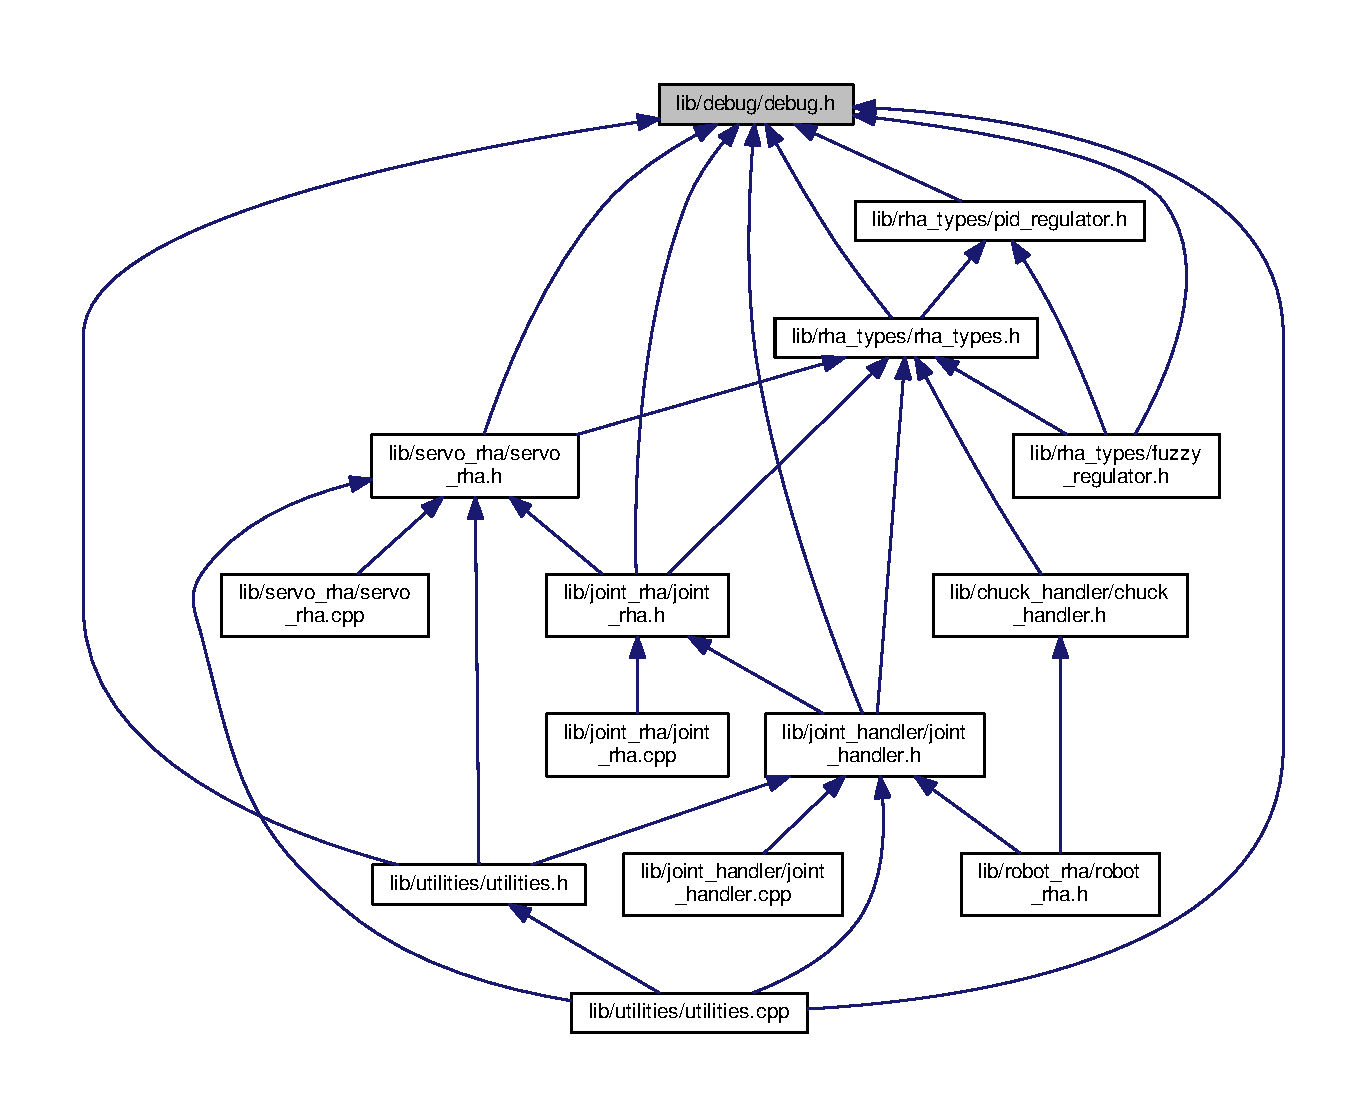
\includegraphics[width=350pt]{debug_8h__dep__incl}
\end{center}
\end{figure}
\subsection*{Macros}
\begin{DoxyCompactItemize}
\item 
\#define {\bfseries D\+E\+B\+U\+G\+\_\+\+T\+E\+S\+T\+\_\+\+S\+E\+R\+V\+O\+\_\+\+R\+H\+A\+\_\+\+R\+E\+AL}\hypertarget{debug_8h_ad967e89fe7d63f8d65f9afd748af37b4}{}\label{debug_8h_ad967e89fe7d63f8d65f9afd748af37b4}

\item 
\#define \hyperlink{debug_8h_a195f4f12e8f7eb49a02c0fdcc3c09254}{Debug\+Serial\+G15\+Ln}(a)
\item 
\#define {\bfseries Debug\+Serial\+G15\+Ln2}(a,  b)\hypertarget{debug_8h_a377cb2bc56545dd0c5344c544af1ec53}{}\label{debug_8h_a377cb2bc56545dd0c5344c544af1ec53}

\item 
\#define {\bfseries Debug\+Serial\+G15\+Ln4}(a,  b,  c,  d)\hypertarget{debug_8h_a0763cacc40537ae208c5cabc821a502a}{}\label{debug_8h_a0763cacc40537ae208c5cabc821a502a}

\item 
\#define \hyperlink{debug_8h_a8c21e78c66c39d131f680bfc750f7cb2}{Debug\+Serial\+S\+R\+H\+A\+Ln}(a)
\item 
\#define {\bfseries Debug\+Serial\+S\+R\+H\+A\+Ln2}(a,  b)\hypertarget{debug_8h_abd539799161c8ef607d721c04e21c9dd}{}\label{debug_8h_abd539799161c8ef607d721c04e21c9dd}

\item 
\#define {\bfseries Debug\+Serial\+S\+R\+H\+A\+Ln4}(a,  b,  c,  d)\hypertarget{debug_8h_a75d23ac365a38dbd2a18037e6f725783}{}\label{debug_8h_a75d23ac365a38dbd2a18037e6f725783}

\item 
\#define \hyperlink{debug_8h_a5252d45d26a7bc560130ef8f12a0716a}{Debug\+Serial\+Utilities\+Ln}(a)
\item 
\#define {\bfseries Debug\+Serial\+Utilities\+Ln2}(a,  b)\hypertarget{debug_8h_a25c02d8c573e390feb1cea152f2f2f44}{}\label{debug_8h_a25c02d8c573e390feb1cea152f2f2f44}

\item 
\#define {\bfseries Debug\+Serial\+Utilities}(a)\hypertarget{debug_8h_af7417e341b05785268a5370629aa29cd}{}\label{debug_8h_af7417e341b05785268a5370629aa29cd}

\item 
\#define {\bfseries Debug\+Serial\+Utilities\+Ln4}(a,  b,  c,  d)\hypertarget{debug_8h_a7991787c91487ea96bbdf717d91ee124}{}\label{debug_8h_a7991787c91487ea96bbdf717d91ee124}

\item 
\#define \hyperlink{debug_8h_ae415bfde264326c977dbceb9c15dbf0b}{Debug\+Serial\+Separation}(a)~\{Serial.\+println(\char`\"{}=========================================================\char`\"{});\}
\item 
\#define \hyperlink{debug_8h_a4c6755ee11caa8cffc48f0dc57a7e3a5}{Debug\+Serial\+T\+G15\+Ln}(a)
\item 
\#define {\bfseries Debug\+Serial\+T\+G15}(a)\hypertarget{debug_8h_ad9046efa7d5554ab69caa28a685ad76c}{}\label{debug_8h_ad9046efa7d5554ab69caa28a685ad76c}

\item 
\#define \hyperlink{debug_8h_a19c59040856e9361f3b041cfd2d6da31}{Debug\+Serial\+T\+S\+R\+H\+A\+Mock\+Ln}(a)
\item 
\#define {\bfseries Debug\+Serial\+T\+S\+R\+H\+A\+Mock}(a)\hypertarget{debug_8h_a14e8d8cb9f05bab7556ea3577444417d}{}\label{debug_8h_a14e8d8cb9f05bab7556ea3577444417d}

\item 
\#define \hyperlink{debug_8h_ac1a1f9f4bd920831ab1c6a4665c6bb98}{Debug\+Serial\+T\+S\+R\+H\+A\+Real\+Ln}(a)~\{  Serial.\+print(\char`\"{}\mbox{[}DT\mbox{]}  (real)Servo\+R\+H\+A\+::\char`\"{}); Serial.\+println(a); \}
\item 
\#define {\bfseries Debug\+Serial\+T\+S\+R\+H\+A\+Real\+Ln2}(a,  b)~\{  Serial.\+print(\char`\"{}\mbox{[}DT\mbox{]}  (real)Servo\+R\+H\+A\+::\char`\"{}); Serial.\+print(a); Serial.\+println(b); \}\hypertarget{debug_8h_a5a434173e97234ecbe1dc2e39b75527e}{}\label{debug_8h_a5a434173e97234ecbe1dc2e39b75527e}

\item 
\#define {\bfseries Debug\+Serial\+T\+S\+R\+H\+A\+Real}(a)~\{  Serial.\+print(\char`\"{}\mbox{[}DT\mbox{]}  (real)Servo\+R\+H\+A\+::\char`\"{}); Serial.\+print(a); \}\hypertarget{debug_8h_aabba0c8959ab9e44abae185ffd5b0ac9}{}\label{debug_8h_aabba0c8959ab9e44abae185ffd5b0ac9}

\item 
\#define {\bfseries Debug\+Serial\+T\+S\+R\+H\+A\+Real\+Ln4}(a,  b,  c,  d)~\{  Serial.\+print(\char`\"{}\mbox{[}DT\mbox{]}  (real)Servo\+R\+H\+A\+::\char`\"{}); Serial.\+print(a); Serial.\+print(b); Serial.\+print(c); Serial.\+println(d); \}\hypertarget{debug_8h_ab87d06e52a63c902e14a7940804aa677}{}\label{debug_8h_ab87d06e52a63c902e14a7940804aa677}

\end{DoxyCompactItemize}


\subsection{Detailed Description}
Implements debugging macros with Serial printig that can be activated or not for each different librari or file. 

Each set of macros has a define option, if it\textquotesingle{}s been defined all debugging options in the set will be printed. If it\textquotesingle{}s not defined Debug commands en that file will be ignored. Each set has different macros which admit different number of parameters to print.

\+: Enrique Heredia Aguado $<$enheragu$>$ \+: 2017\+\_\+\+Sep\+\_\+08 \+: R\+HA \+: \hyperlink{debug_8h}{debug.\+h}  modified by\+: enheragu  modified time\+: 08\+\_\+\+Sep\+\_\+2017 

\subsection{Macro Definition Documentation}
\index{debug.\+h@{debug.\+h}!Debug\+Serial\+G15\+Ln@{Debug\+Serial\+G15\+Ln}}
\index{Debug\+Serial\+G15\+Ln@{Debug\+Serial\+G15\+Ln}!debug.\+h@{debug.\+h}}
\subsubsection[{\texorpdfstring{Debug\+Serial\+G15\+Ln}{DebugSerialG15Ln}}]{\setlength{\rightskip}{0pt plus 5cm}\#define Debug\+Serial\+G15\+Ln(
\begin{DoxyParamCaption}
\item[{}]{a}
\end{DoxyParamCaption}
)}\hypertarget{debug_8h_a195f4f12e8f7eb49a02c0fdcc3c09254}{}\label{debug_8h_a195f4f12e8f7eb49a02c0fdcc3c09254}
D\+E\+B\+U\+G\+\_\+\+C\+Y\+T\+R\+O\+N\+\_\+\+G15\+\_\+\+S\+E\+R\+VO implements debug macros for \hyperlink{cytron__g15__servo_8h_source}{cytron\+\_\+g15\+\_\+servo.\+h} and .cpp files \index{debug.\+h@{debug.\+h}!Debug\+Serial\+Separation@{Debug\+Serial\+Separation}}
\index{Debug\+Serial\+Separation@{Debug\+Serial\+Separation}!debug.\+h@{debug.\+h}}
\subsubsection[{\texorpdfstring{Debug\+Serial\+Separation}{DebugSerialSeparation}}]{\setlength{\rightskip}{0pt plus 5cm}\#define Debug\+Serial\+Separation(
\begin{DoxyParamCaption}
\item[{}]{a}
\end{DoxyParamCaption}
)~\{Serial.\+println(\char`\"{}=========================================================\char`\"{});\}}\hypertarget{debug_8h_ae415bfde264326c977dbceb9c15dbf0b}{}\label{debug_8h_ae415bfde264326c977dbceb9c15dbf0b}
Debug\+Serial\+Separation prints a horizontal line to separate different set of debug information \index{debug.\+h@{debug.\+h}!Debug\+Serial\+S\+R\+H\+A\+Ln@{Debug\+Serial\+S\+R\+H\+A\+Ln}}
\index{Debug\+Serial\+S\+R\+H\+A\+Ln@{Debug\+Serial\+S\+R\+H\+A\+Ln}!debug.\+h@{debug.\+h}}
\subsubsection[{\texorpdfstring{Debug\+Serial\+S\+R\+H\+A\+Ln}{DebugSerialSRHALn}}]{\setlength{\rightskip}{0pt plus 5cm}\#define Debug\+Serial\+S\+R\+H\+A\+Ln(
\begin{DoxyParamCaption}
\item[{}]{a}
\end{DoxyParamCaption}
)}\hypertarget{debug_8h_a8c21e78c66c39d131f680bfc750f7cb2}{}\label{debug_8h_a8c21e78c66c39d131f680bfc750f7cb2}
D\+E\+B\+U\+G\+\_\+\+S\+E\+R\+V\+O\+\_\+\+R\+HA implements debug macros for \hyperlink{servo__rha_8h}{servo\+\_\+rha.\+h} and .cpp files \index{debug.\+h@{debug.\+h}!Debug\+Serial\+T\+G15\+Ln@{Debug\+Serial\+T\+G15\+Ln}}
\index{Debug\+Serial\+T\+G15\+Ln@{Debug\+Serial\+T\+G15\+Ln}!debug.\+h@{debug.\+h}}
\subsubsection[{\texorpdfstring{Debug\+Serial\+T\+G15\+Ln}{DebugSerialTG15Ln}}]{\setlength{\rightskip}{0pt plus 5cm}\#define Debug\+Serial\+T\+G15\+Ln(
\begin{DoxyParamCaption}
\item[{}]{a}
\end{DoxyParamCaption}
)}\hypertarget{debug_8h_a4c6755ee11caa8cffc48f0dc57a7e3a5}{}\label{debug_8h_a4c6755ee11caa8cffc48f0dc57a7e3a5}
D\+E\+B\+U\+G\+\_\+\+T\+E\+S\+T\+\_\+\+C\+Y\+T\+R\+O\+N\+\_\+\+G15\+\_\+\+S\+E\+R\+VO implements debug macros for test\+\_\+cytron\+\_\+g15\+\_\+servo.\+cpp file \index{debug.\+h@{debug.\+h}!Debug\+Serial\+T\+S\+R\+H\+A\+Mock\+Ln@{Debug\+Serial\+T\+S\+R\+H\+A\+Mock\+Ln}}
\index{Debug\+Serial\+T\+S\+R\+H\+A\+Mock\+Ln@{Debug\+Serial\+T\+S\+R\+H\+A\+Mock\+Ln}!debug.\+h@{debug.\+h}}
\subsubsection[{\texorpdfstring{Debug\+Serial\+T\+S\+R\+H\+A\+Mock\+Ln}{DebugSerialTSRHAMockLn}}]{\setlength{\rightskip}{0pt plus 5cm}\#define Debug\+Serial\+T\+S\+R\+H\+A\+Mock\+Ln(
\begin{DoxyParamCaption}
\item[{}]{a}
\end{DoxyParamCaption}
)}\hypertarget{debug_8h_a19c59040856e9361f3b041cfd2d6da31}{}\label{debug_8h_a19c59040856e9361f3b041cfd2d6da31}
D\+E\+B\+U\+G\+\_\+\+T\+E\+S\+T\+\_\+\+S\+E\+R\+V\+O\+\_\+\+R\+H\+A\+\_\+\+M\+O\+CK implements debug macros for test\+\_\+servo\+\_\+mock.\+cpp file \index{debug.\+h@{debug.\+h}!Debug\+Serial\+T\+S\+R\+H\+A\+Real\+Ln@{Debug\+Serial\+T\+S\+R\+H\+A\+Real\+Ln}}
\index{Debug\+Serial\+T\+S\+R\+H\+A\+Real\+Ln@{Debug\+Serial\+T\+S\+R\+H\+A\+Real\+Ln}!debug.\+h@{debug.\+h}}
\subsubsection[{\texorpdfstring{Debug\+Serial\+T\+S\+R\+H\+A\+Real\+Ln}{DebugSerialTSRHARealLn}}]{\setlength{\rightskip}{0pt plus 5cm}\#define Debug\+Serial\+T\+S\+R\+H\+A\+Real\+Ln(
\begin{DoxyParamCaption}
\item[{}]{a}
\end{DoxyParamCaption}
)~\{  Serial.\+print(\char`\"{}\mbox{[}DT\mbox{]}  (real)Servo\+R\+H\+A\+::\char`\"{}); Serial.\+println(a); \}}\hypertarget{debug_8h_ac1a1f9f4bd920831ab1c6a4665c6bb98}{}\label{debug_8h_ac1a1f9f4bd920831ab1c6a4665c6bb98}
D\+E\+B\+U\+G\+\_\+\+T\+E\+S\+T\+\_\+\+S\+E\+R\+V\+O\+\_\+\+R\+H\+A\+\_\+\+R\+E\+AL implements debug macros for test\+\_\+servo\+\_\+real.\+cpp file \index{debug.\+h@{debug.\+h}!Debug\+Serial\+Utilities\+Ln@{Debug\+Serial\+Utilities\+Ln}}
\index{Debug\+Serial\+Utilities\+Ln@{Debug\+Serial\+Utilities\+Ln}!debug.\+h@{debug.\+h}}
\subsubsection[{\texorpdfstring{Debug\+Serial\+Utilities\+Ln}{DebugSerialUtilitiesLn}}]{\setlength{\rightskip}{0pt plus 5cm}\#define Debug\+Serial\+Utilities\+Ln(
\begin{DoxyParamCaption}
\item[{}]{a}
\end{DoxyParamCaption}
)}\hypertarget{debug_8h_a5252d45d26a7bc560130ef8f12a0716a}{}\label{debug_8h_a5252d45d26a7bc560130ef8f12a0716a}
D\+E\+B\+U\+G\+\_\+\+U\+T\+I\+L\+I\+T\+I\+ES implements debug macros for \hyperlink{utilities_8h}{utilities.\+h} file 
\hypertarget{joint__handler_8cpp}{}\section{lib/joint\+\_\+handler/joint\+\_\+handler.cpp File Reference}
\label{joint__handler_8cpp}\index{lib/joint\+\_\+handler/joint\+\_\+handler.\+cpp@{lib/joint\+\_\+handler/joint\+\_\+handler.\+cpp}}


Implements \hyperlink{classJointHandler}{Joint\+Handler} functions defined in \hyperlink{joint__handler_8h}{joint\+\_\+handler.\+h}.  


{\ttfamily \#include \char`\"{}joint\+\_\+handler.\+h\char`\"{}}\\*
Include dependency graph for joint\+\_\+handler.\+cpp\+:
\nopagebreak
\begin{figure}[H]
\begin{center}
\leavevmode
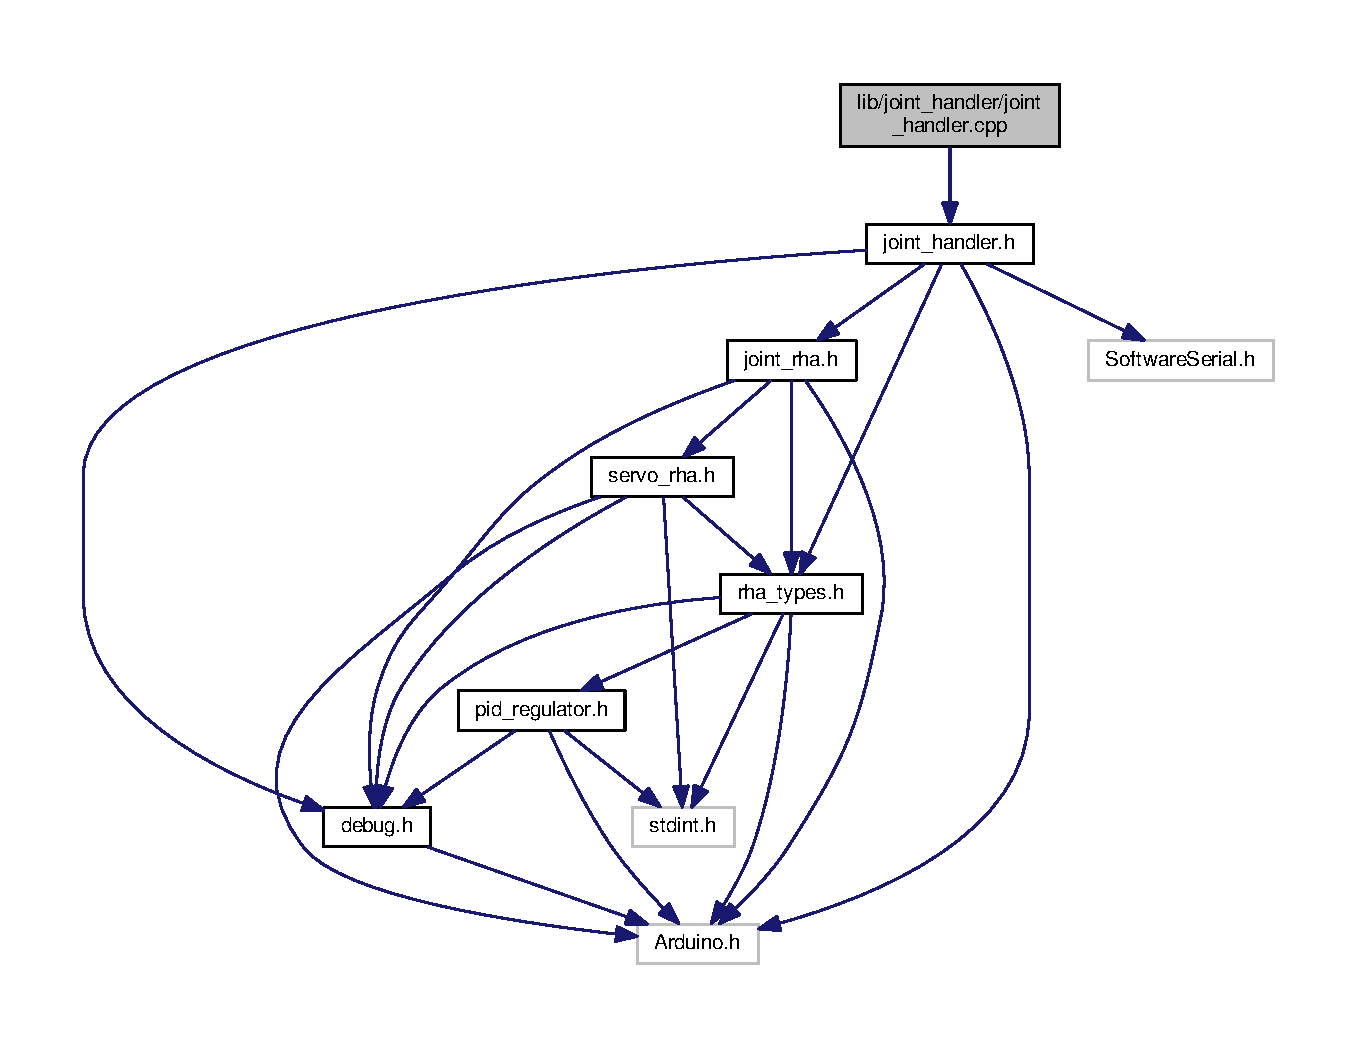
\includegraphics[width=350pt]{joint__handler_8cpp__incl}
\end{center}
\end{figure}
\subsection*{Variables}
\begin{DoxyCompactItemize}
\item 
boolean {\bfseries hardware\+Serial\+\_\+} = false\hypertarget{joint__handler_8cpp_a4f95f8b28db77eb6cd529511e9cc953c}{}\label{joint__handler_8cpp_a4f95f8b28db77eb6cd529511e9cc953c}

\item 
Software\+Serial $\ast$ {\bfseries G15\+Serial\+\_\+}\hypertarget{joint__handler_8cpp_ad5b8fd79a7e7700773ecd1201d5cd1e1}{}\label{joint__handler_8cpp_ad5b8fd79a7e7700773ecd1201d5cd1e1}

\end{DoxyCompactItemize}


\subsection{Detailed Description}
Implements \hyperlink{classJointHandler}{Joint\+Handler} functions defined in \hyperlink{joint__handler_8h}{joint\+\_\+handler.\+h}. 

\+: Enrique Heredia Aguado $<$enheragu$>$ \+: 2017\+\_\+\+Sep\+\_\+08 \+: R\+HA \+: \hyperlink{joint__handler_8cpp}{joint\+\_\+handler.\+cpp}  modified by\+: enheragu  modified time\+: 31\+\_\+\+Oct\+\_\+2017 
\hypertarget{joint__handler_8h}{}\section{lib/joint\+\_\+handler/joint\+\_\+handler.h File Reference}
\label{joint__handler_8h}\index{lib/joint\+\_\+handler/joint\+\_\+handler.\+h@{lib/joint\+\_\+handler/joint\+\_\+handler.\+h}}


Implements \hyperlink{classJointHandler}{Joint\+Handler} class. This object is in charge to sync all joints.  


{\ttfamily \#include \char`\"{}joint\+\_\+rha.\+h\char`\"{}}\\*
Include dependency graph for joint\+\_\+handler.\+h\+:\nopagebreak
\begin{figure}[H]
\begin{center}
\leavevmode
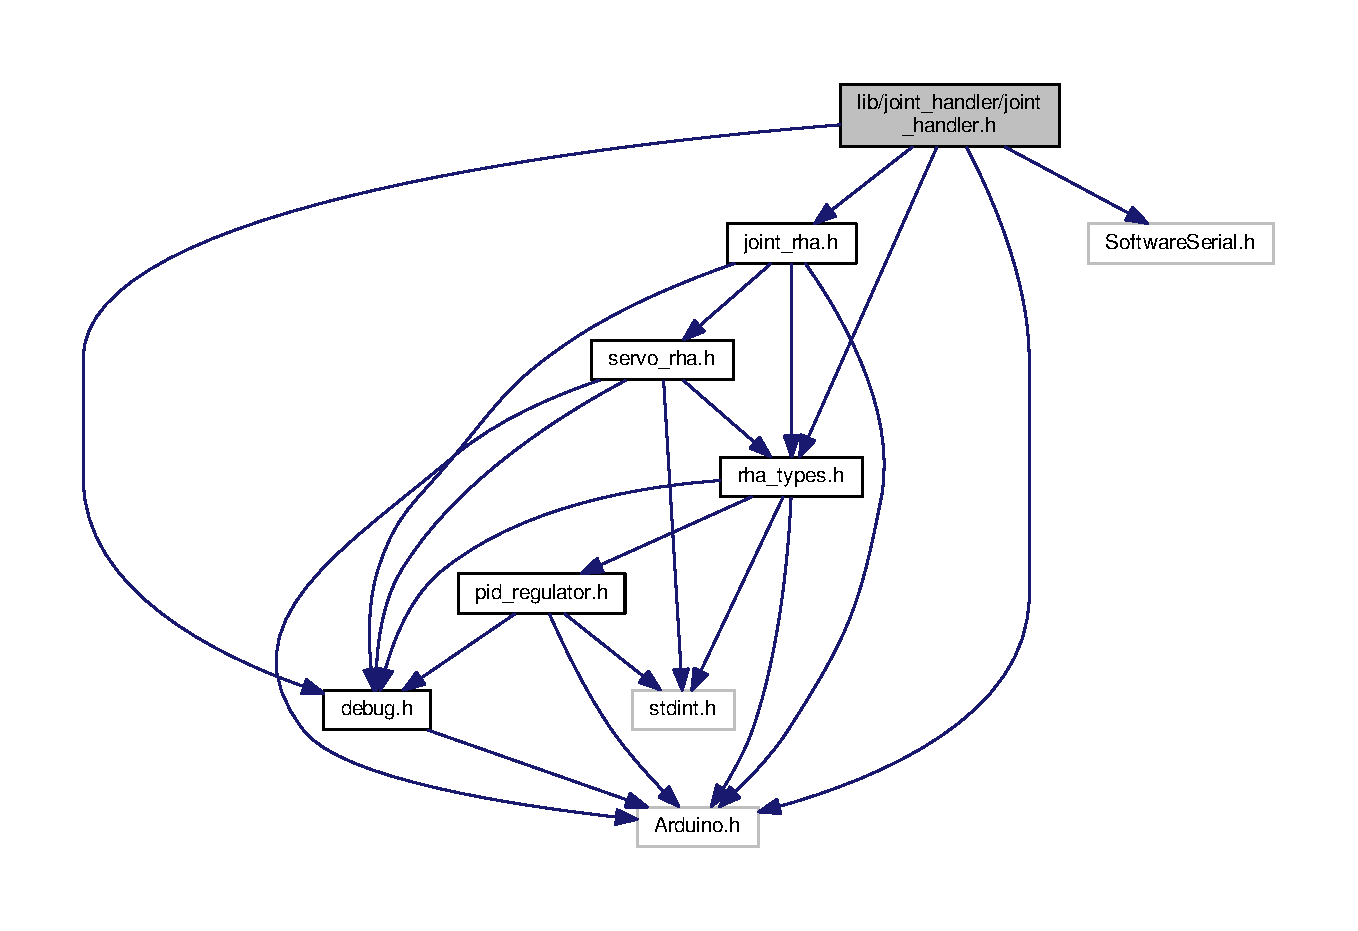
\includegraphics[width=314pt]{joint__handler_8h__incl}
\end{center}
\end{figure}
This graph shows which files directly or indirectly include this file\+:\nopagebreak
\begin{figure}[H]
\begin{center}
\leavevmode
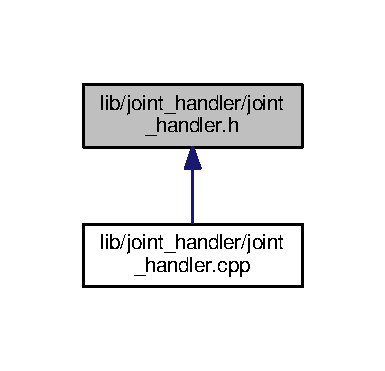
\includegraphics[width=185pt]{joint__handler_8h__dep__incl}
\end{center}
\end{figure}
\subsection*{Classes}
\begin{DoxyCompactItemize}
\item 
class \hyperlink{classJointHandler}{Joint\+Handler}
\end{DoxyCompactItemize}


\subsection{Detailed Description}
Implements \hyperlink{classJointHandler}{Joint\+Handler} class. This object is in charge to sync all joints. 

\+: Enrique Heredia Aguado $<$enheragu$>$ \+: 2017\+\_\+\+Sep\+\_\+08 \+: R\+HA \+: \hyperlink{joint__handler_8h}{joint\+\_\+handler.\+h}  modified by\+: enheragu  modified time\+: 08\+\_\+\+Sep\+\_\+2017 
\hypertarget{joint__rha_8cpp}{}\section{lib/joint\+\_\+rha/joint\+\_\+rha.cpp File Reference}
\label{joint__rha_8cpp}\index{lib/joint\+\_\+rha/joint\+\_\+rha.\+cpp@{lib/joint\+\_\+rha/joint\+\_\+rha.\+cpp}}


Implements \hyperlink{classJointRHA}{Joint\+R\+HA} functions defined in \hyperlink{joint__rha_8h}{joint\+\_\+rha.\+h} \+: Enrique Heredia Aguado $<$enheragu$>$ \+: 2017\+\_\+\+Sep\+\_\+08 \+: R\+HA \+: \hyperlink{joint__rha_8cpp}{joint\+\_\+rha.\+cpp}  modified by\+: enheragu  modified time\+: 08\+\_\+\+Sep\+\_\+2017.  


{\ttfamily \#include \char`\"{}joint\+\_\+rha.\+h\char`\"{}}\\*
Include dependency graph for joint\+\_\+rha.\+cpp\+:\nopagebreak
\begin{figure}[H]
\begin{center}
\leavevmode
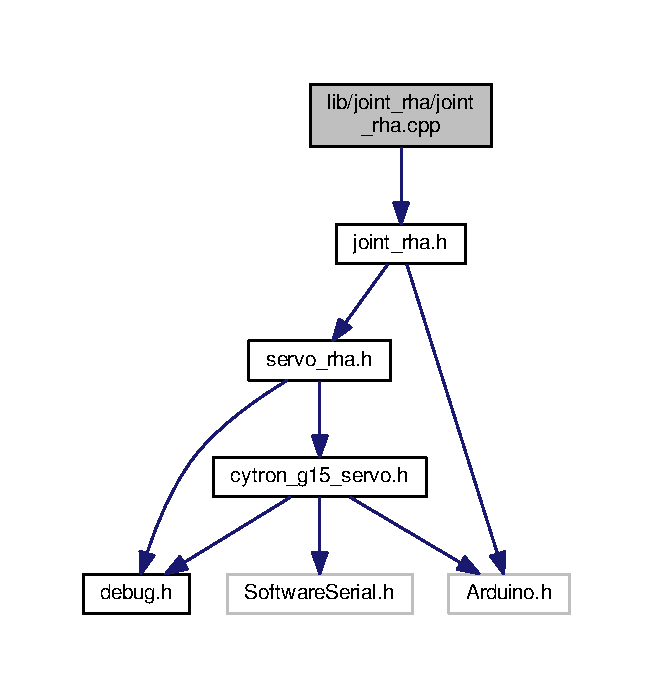
\includegraphics[width=314pt]{joint__rha_8cpp__incl}
\end{center}
\end{figure}
\subsection*{Functions}
\begin{DoxyCompactItemize}
\item 
uint16\+\_\+t {\bfseries send\+Packet} (uint8\+\_\+t instruction, uint8\+\_\+t $\ast$data, uint8\+\_\+t parameter\+Length)\hypertarget{joint__rha_8cpp_ade1c41e09e51c36b1635f7835813d02a}{}\label{joint__rha_8cpp_ade1c41e09e51c36b1635f7835813d02a}

\end{DoxyCompactItemize}


\subsection{Detailed Description}
Implements \hyperlink{classJointRHA}{Joint\+R\+HA} functions defined in \hyperlink{joint__rha_8h}{joint\+\_\+rha.\+h} \+: Enrique Heredia Aguado $<$enheragu$>$ \+: 2017\+\_\+\+Sep\+\_\+08 \+: R\+HA \+: \hyperlink{joint__rha_8cpp}{joint\+\_\+rha.\+cpp}  modified by\+: enheragu  modified time\+: 08\+\_\+\+Sep\+\_\+2017. 


\hypertarget{joint__rha_8h}{}\section{lib/joint\+\_\+rha/joint\+\_\+rha.h File Reference}
\label{joint__rha_8h}\index{lib/joint\+\_\+rha/joint\+\_\+rha.\+h@{lib/joint\+\_\+rha/joint\+\_\+rha.\+h}}


Implements \hyperlink{classJointRHA}{Joint\+R\+HA} class. This object combines potentiometer with \hyperlink{classServoRHA}{Servo\+R\+HA} object readings to enhance it\textquotesingle{}s functionality.  


{\ttfamily \#include \char`\"{}servo\+\_\+rha.\+h\char`\"{}}\\*
{\ttfamily \#include \char`\"{}rha\+\_\+types.\+h\char`\"{}}\\*
{\ttfamily \#include \char`\"{}debug.\+h\char`\"{}}\\*
{\ttfamily \#include \char`\"{}Arduino.\+h\char`\"{}}\\*
Include dependency graph for joint\+\_\+rha.\+h\+:
\nopagebreak
\begin{figure}[H]
\begin{center}
\leavevmode
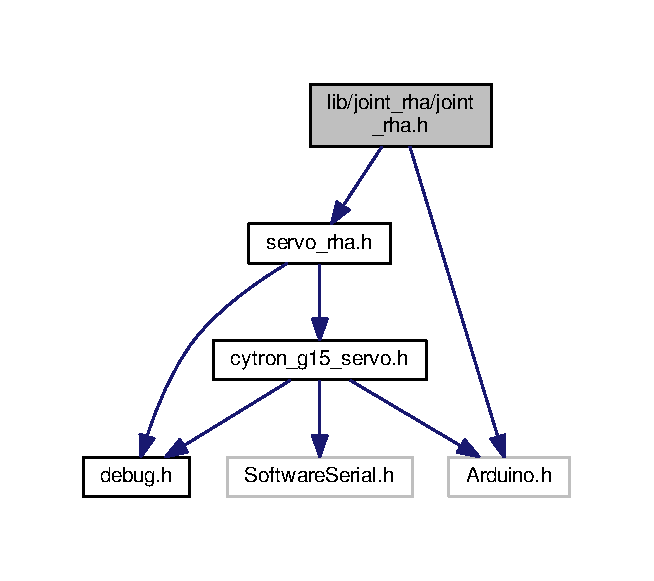
\includegraphics[width=350pt]{joint__rha_8h__incl}
\end{center}
\end{figure}
This graph shows which files directly or indirectly include this file\+:
\nopagebreak
\begin{figure}[H]
\begin{center}
\leavevmode
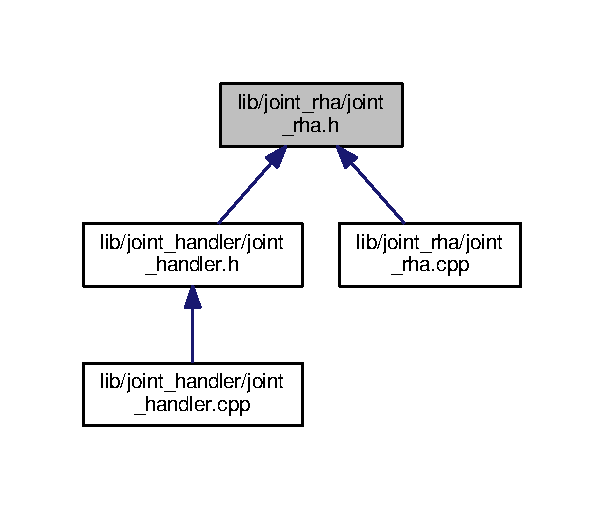
\includegraphics[width=350pt]{joint__rha_8h__dep__incl}
\end{center}
\end{figure}
\subsection*{Classes}
\begin{DoxyCompactItemize}
\item 
class \hyperlink{classJointRHA}{Joint\+R\+HA}
\end{DoxyCompactItemize}
\subsection*{Macros}
\begin{DoxyCompactItemize}
\item 
\#define {\bfseries A\+N\+G\+L\+E\+\_\+\+T\+O\+L\+E\+R\+A\+N\+CE}~4\hypertarget{joint__rha_8h_a5835d2253221816d4f18e65f9796d3c6}{}\label{joint__rha_8h_a5835d2253221816d4f18e65f9796d3c6}

\item 
\#define {\bfseries N\+O\+\_\+\+P\+O\+T\+E\+N\+T\+I\+O\+M\+E\+T\+ER}~255\hypertarget{joint__rha_8h_addf193ce825d9ffa5de2292c35048697}{}\label{joint__rha_8h_addf193ce825d9ffa5de2292c35048697}

\item 
\#define \hyperlink{joint__rha_8h_a4831340c66d074adb5481fc3ad5a2e65}{E\+R\+R\+O\+R\+\_\+\+M\+O\+V\+I\+N\+G\+\_\+\+M\+A\+R\+G\+IN}~5
\item 
\#define {\bfseries KP}~0.\+35\hypertarget{joint__rha_8h_aa4729260b732666338dee7d841aa12f3}{}\label{joint__rha_8h_aa4729260b732666338dee7d841aa12f3}

\item 
\#define {\bfseries KD}~1\hypertarget{joint__rha_8h_ad4f9673d16d231643789f081068d2372}{}\label{joint__rha_8h_ad4f9673d16d231643789f081068d2372}

\item 
\#define {\bfseries KI}~1\hypertarget{joint__rha_8h_ade82752ae1652fdf0df9df7a16ffda29}{}\label{joint__rha_8h_ade82752ae1652fdf0df9df7a16ffda29}

\end{DoxyCompactItemize}


\subsection{Detailed Description}
Implements \hyperlink{classJointRHA}{Joint\+R\+HA} class. This object combines potentiometer with \hyperlink{classServoRHA}{Servo\+R\+HA} object readings to enhance it\textquotesingle{}s functionality. 

\+: Enrique Heredia Aguado $<$enheragu$>$ \+: 2017\+\_\+\+Sep\+\_\+08 \+: R\+HA \+: \hyperlink{joint__rha_8h}{joint\+\_\+rha.\+h}  modified by\+: quique  modified time\+: 29-\/\+Sep-\/2017 

\subsection{Macro Definition Documentation}
\index{joint\+\_\+rha.\+h@{joint\+\_\+rha.\+h}!E\+R\+R\+O\+R\+\_\+\+M\+O\+V\+I\+N\+G\+\_\+\+M\+A\+R\+G\+IN@{E\+R\+R\+O\+R\+\_\+\+M\+O\+V\+I\+N\+G\+\_\+\+M\+A\+R\+G\+IN}}
\index{E\+R\+R\+O\+R\+\_\+\+M\+O\+V\+I\+N\+G\+\_\+\+M\+A\+R\+G\+IN@{E\+R\+R\+O\+R\+\_\+\+M\+O\+V\+I\+N\+G\+\_\+\+M\+A\+R\+G\+IN}!joint\+\_\+rha.\+h@{joint\+\_\+rha.\+h}}
\subsubsection[{\texorpdfstring{E\+R\+R\+O\+R\+\_\+\+M\+O\+V\+I\+N\+G\+\_\+\+M\+A\+R\+G\+IN}{ERROR_MOVING_MARGIN}}]{\setlength{\rightskip}{0pt plus 5cm}\#define E\+R\+R\+O\+R\+\_\+\+M\+O\+V\+I\+N\+G\+\_\+\+M\+A\+R\+G\+IN~5}\hypertarget{joint__rha_8h_a4831340c66d074adb5481fc3ad5a2e65}{}\label{joint__rha_8h_a4831340c66d074adb5481fc3ad5a2e65}
It the servo moves but not the joint for more than E\+R\+R\+O\+R\+\_\+\+M\+O\+V\+I\+N\+G\+\_\+\+M\+A\+R\+G\+IN cicles it raiseses an error 
\hypertarget{servo__rha_8cpp}{}\section{lib/servo\+\_\+rha/servo\+\_\+rha.cpp File Reference}
\label{servo__rha_8cpp}\index{lib/servo\+\_\+rha/servo\+\_\+rha.\+cpp@{lib/servo\+\_\+rha/servo\+\_\+rha.\+cpp}}


Implements \hyperlink{classServoRHA}{Servo\+R\+HA} functions defined in \hyperlink{servo__rha_8h}{servo\+\_\+rha.\+h}.  


{\ttfamily \#include \char`\"{}servo\+\_\+rha.\+h\char`\"{}}\\*
{\ttfamily \#include \char`\"{}cytron\+\_\+g15\+\_\+servo.\+h\char`\"{}}\\*
{\ttfamily \#include \char`\"{}Arduino.\+h\char`\"{}}\\*
Include dependency graph for servo\+\_\+rha.\+cpp\+:\nopagebreak
\begin{figure}[H]
\begin{center}
\leavevmode
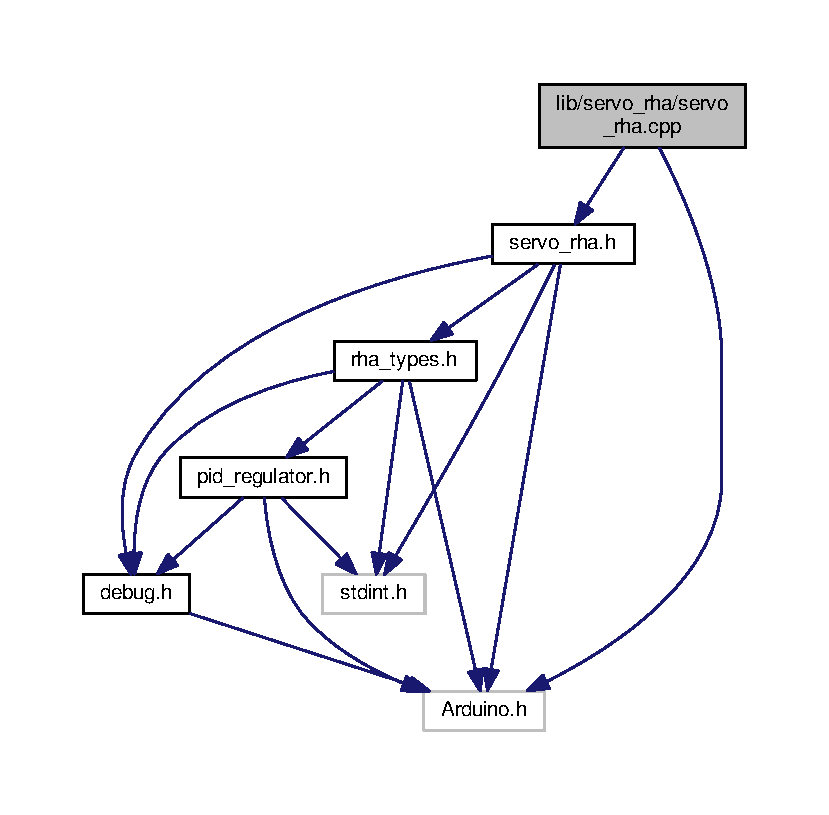
\includegraphics[width=314pt]{servo__rha_8cpp__incl}
\end{center}
\end{figure}
\subsection*{Functions}
\begin{DoxyCompactItemize}
\item 
uint16\+\_\+t {\bfseries regulator\+Servo} (uint16\+\_\+t error, uint8\+\_\+t kp)\hypertarget{servo__rha_8cpp_af0af842f10161b9ff04104036dd51ea1}{}\label{servo__rha_8cpp_af0af842f10161b9ff04104036dd51ea1}

\item 
uint8\+\_\+t \hyperlink{servo__rha_8cpp_a423942587cd078cd1dc677829e34cb18}{compare\+Angles} (uint16\+\_\+t angle1, uint16\+\_\+t angle2, uint8\+\_\+t angle\+\_\+margin)
\begin{DoxyCompactList}\small\item\em compare\+Angles function compares two angles with a margin set. \end{DoxyCompactList}\item 
uint8\+\_\+t \hyperlink{servo__rha_8cpp_ac74e39c3dac1d2fc9ff05f10fb898042}{compare\+Speed} (uint16\+\_\+t speed1, uint16\+\_\+t speed2, uint8\+\_\+t speed\+\_\+margin)
\begin{DoxyCompactList}\small\item\em compare\+Speed function compares two speeds with a margin set. \end{DoxyCompactList}\end{DoxyCompactItemize}


\subsection{Detailed Description}
Implements \hyperlink{classServoRHA}{Servo\+R\+HA} functions defined in \hyperlink{servo__rha_8h}{servo\+\_\+rha.\+h}. 

\+: Enrique Heredia Aguado $<$enheragu$>$ \+: 2017\+\_\+\+Sep\+\_\+08 \+: R\+HA \+: \hyperlink{servo__rha_8cpp}{servo\+\_\+rha.\+cpp}  modified by\+: enheragu  modified time\+: 09-\/\+Sep-\/2017 

\subsection{Function Documentation}
\index{servo\+\_\+rha.\+cpp@{servo\+\_\+rha.\+cpp}!compare\+Angles@{compare\+Angles}}
\index{compare\+Angles@{compare\+Angles}!servo\+\_\+rha.\+cpp@{servo\+\_\+rha.\+cpp}}
\subsubsection[{\texorpdfstring{compare\+Angles(uint16\+\_\+t angle1, uint16\+\_\+t angle2, uint8\+\_\+t angle\+\_\+margin)}{compareAngles(uint16_t angle1, uint16_t angle2, uint8_t angle_margin)}}]{\setlength{\rightskip}{0pt plus 5cm}uint8\+\_\+t compare\+Angles (
\begin{DoxyParamCaption}
\item[{uint16\+\_\+t}]{angle1, }
\item[{uint16\+\_\+t}]{angle2, }
\item[{uint8\+\_\+t}]{angle\+\_\+margin}
\end{DoxyParamCaption}
)}\hypertarget{servo__rha_8cpp_a423942587cd078cd1dc677829e34cb18}{}\label{servo__rha_8cpp_a423942587cd078cd1dc677829e34cb18}


compare\+Angles function compares two angles with a margin set. 


\begin{DoxyParams}{Parameters}
{\em \{uint16\+\_\+t\}} & angle1\+: angle to compare \\
\hline
{\em \{uint16\+\_\+t\}} & angle2\+: angle used in the comparison \\
\hline
{\em \{uint8\+\_\+t\}} & angle\+\_\+margin\+: margin in which the angle1 will be considered to be equal to angle2 \mbox{[}angle2-\/angle\+\_\+margin, angle2+angle\+\_\+margin\mbox{]} \\
\hline
\end{DoxyParams}
\begin{DoxyReturn}{Returns}
\{uint8\+\_\+t\} Returns enumeration defined in \hyperlink{servo__rha_8h}{servo\+\_\+rha.\+h} -\/$>$ L\+E\+S\+S\+\_\+\+T\+H\+AN, G\+R\+E\+A\+T\+E\+R\+\_\+\+T\+H\+AN or E\+Q\+U\+AL 
\end{DoxyReturn}
\index{servo\+\_\+rha.\+cpp@{servo\+\_\+rha.\+cpp}!compare\+Speed@{compare\+Speed}}
\index{compare\+Speed@{compare\+Speed}!servo\+\_\+rha.\+cpp@{servo\+\_\+rha.\+cpp}}
\subsubsection[{\texorpdfstring{compare\+Speed(uint16\+\_\+t speed1, uint16\+\_\+t speed2, uint8\+\_\+t speed\+\_\+margin)}{compareSpeed(uint16_t speed1, uint16_t speed2, uint8_t speed_margin)}}]{\setlength{\rightskip}{0pt plus 5cm}uint8\+\_\+t compare\+Speed (
\begin{DoxyParamCaption}
\item[{uint16\+\_\+t}]{speed1, }
\item[{uint16\+\_\+t}]{speed2, }
\item[{uint8\+\_\+t}]{speed\+\_\+margin}
\end{DoxyParamCaption}
)}\hypertarget{servo__rha_8cpp_ac74e39c3dac1d2fc9ff05f10fb898042}{}\label{servo__rha_8cpp_ac74e39c3dac1d2fc9ff05f10fb898042}


compare\+Speed function compares two speeds with a margin set. 


\begin{DoxyParams}{Parameters}
{\em \{uint16\+\_\+t\}} & speed1\+: speed to compare \\
\hline
{\em \{uint16\+\_\+t\}} & speed2\+: speed used in the comparison \\
\hline
{\em \{uint8\+\_\+t\}} & speed\+\_\+margin\+: margin in which the speed will be considered to be equal to speed2 \mbox{[}speed2-\/speed\+\_\+margin, speed2+speed\+\_\+margin\mbox{]} \\
\hline
\end{DoxyParams}
\begin{DoxyReturn}{Returns}
\{uint8\+\_\+t\} Returns enumeration defined in \hyperlink{servo__rha_8h}{servo\+\_\+rha.\+h} -\/$>$ L\+E\+S\+S\+\_\+\+T\+H\+AN, G\+R\+E\+A\+T\+E\+R\+\_\+\+T\+H\+AN or E\+Q\+U\+AL 
\end{DoxyReturn}

\hypertarget{servo__rha_8h}{}\section{lib/servo\+\_\+rha/servo\+\_\+rha.h File Reference}
\label{servo__rha_8h}\index{lib/servo\+\_\+rha/servo\+\_\+rha.\+h@{lib/servo\+\_\+rha/servo\+\_\+rha.\+h}}


Implements \hyperlink{classServoRHA}{Servo\+R\+HA} class. This object inherits from Cytron\+G15\+Servo object to enhance its capabilities.  


{\ttfamily \#include \char`\"{}debug.\+h\char`\"{}}\\*
{\ttfamily \#include \char`\"{}cytron\+\_\+g15\+\_\+servo.\+h\char`\"{}}\\*
Include dependency graph for servo\+\_\+rha.\+h\+:\nopagebreak
\begin{figure}[H]
\begin{center}
\leavevmode
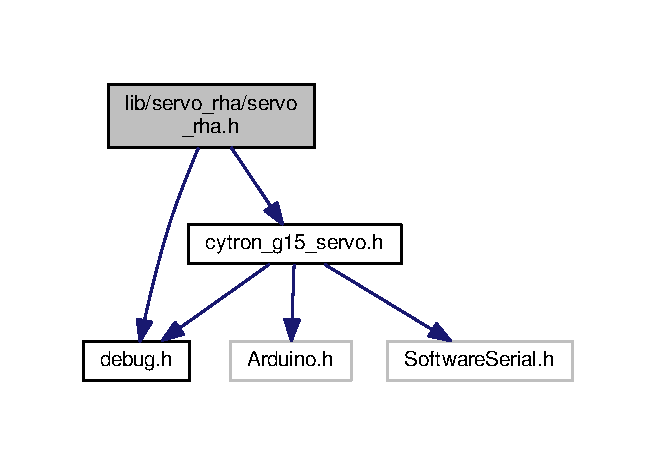
\includegraphics[width=315pt]{servo__rha_8h__incl}
\end{center}
\end{figure}
This graph shows which files directly or indirectly include this file\+:\nopagebreak
\begin{figure}[H]
\begin{center}
\leavevmode
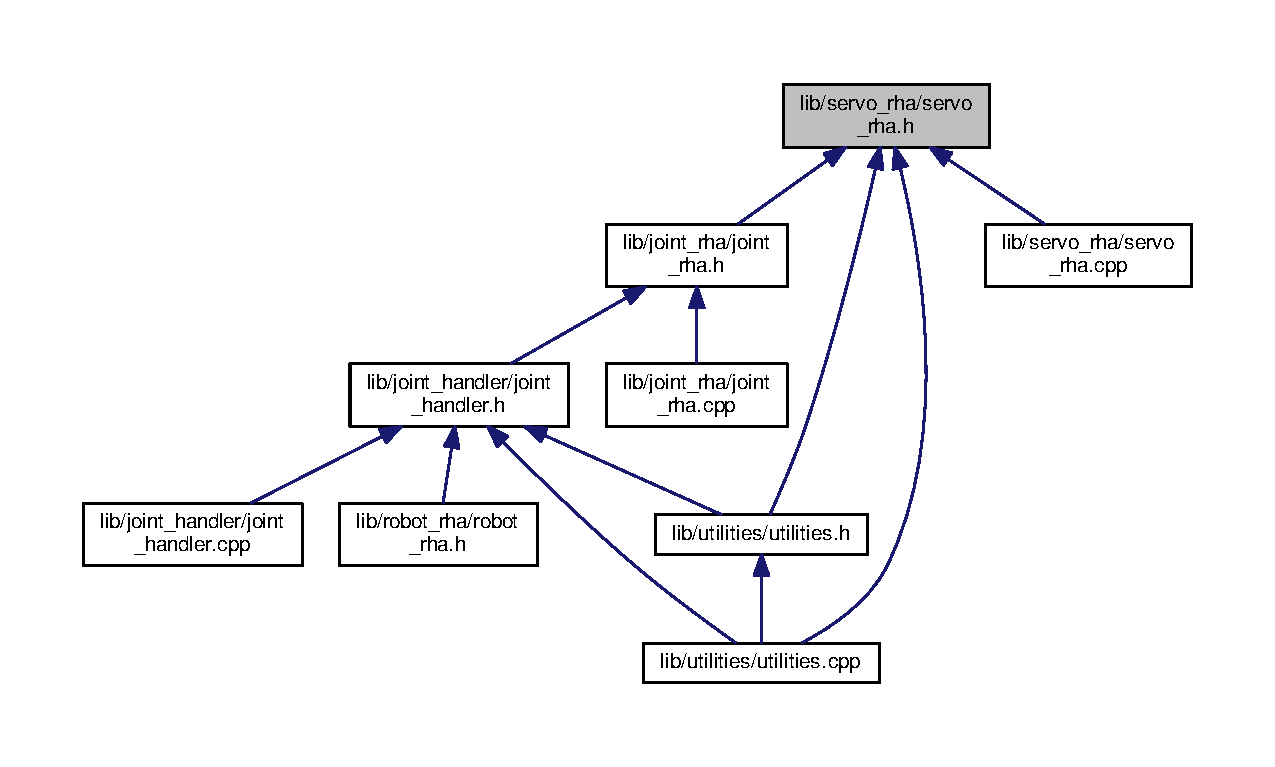
\includegraphics[width=350pt]{servo__rha_8h__dep__incl}
\end{center}
\end{figure}
\subsection*{Classes}
\begin{DoxyCompactItemize}
\item 
class \hyperlink{classServoRHA}{Servo\+R\+HA}
\end{DoxyCompactItemize}
\subsection*{Macros}
\begin{DoxyCompactItemize}
\item 
\#define {\bfseries D\+E\+L\+A\+Y1}~500\hypertarget{servo__rha_8h_a8c5d5597c8e7b779bcd00098025b4905}{}\label{servo__rha_8h_a8c5d5597c8e7b779bcd00098025b4905}

\item 
\#define {\bfseries T\+O\+R\+Q\+U\+E\+\_\+\+C\+A\+L\+I\+B\+R\+A\+T\+I\+O\+N\+\_\+\+I\+N\+T\+E\+R\+V\+AL}~5\hypertarget{servo__rha_8h_a15567874abe1ab88fd408bd5a6fec947}{}\label{servo__rha_8h_a15567874abe1ab88fd408bd5a6fec947}

\item 
\#define {\bfseries M\+I\+N\+\_\+\+T\+O\+R\+Q\+U\+E\+\_\+\+C\+A\+L\+I\+B\+R\+A\+T\+I\+ON}~0\hypertarget{servo__rha_8h_a15ad7f13fbab5c30ae49a984b2db2b2f}{}\label{servo__rha_8h_a15ad7f13fbab5c30ae49a984b2db2b2f}

\item 
\#define {\bfseries M\+A\+X\+\_\+\+T\+O\+R\+Q\+U\+E\+\_\+\+C\+A\+L\+I\+B\+R\+A\+T\+I\+ON}~800\hypertarget{servo__rha_8h_afe501bd33b0f43492c4f5486e3d50654}{}\label{servo__rha_8h_afe501bd33b0f43492c4f5486e3d50654}

\item 
\#define \hyperlink{servo__rha_8h_adfcd13f071007e5e2d089e1593617ac0}{M\+A\+R\+G\+I\+N\+\_\+\+S\+P\+E\+E\+D\+\_\+\+C\+O\+M\+P\+A\+R\+I\+S\+ON}~5
\item 
\#define \hyperlink{servo__rha_8h_ab158bc5ac34a0aceda58d77c83e02724}{M\+A\+R\+G\+I\+N\+\_\+\+A\+N\+G\+L\+E\+\_\+\+C\+O\+M\+P\+A\+R\+I\+S\+ON}~5
\item 
\#define {\bfseries M\+I\+N\+\_\+\+T\+O\+R\+Q\+U\+E\+\_\+\+CW}~0\hypertarget{servo__rha_8h_adcad8252ee1a8885c8f4d4576266a447}{}\label{servo__rha_8h_adcad8252ee1a8885c8f4d4576266a447}

\item 
\#define {\bfseries M\+I\+N\+\_\+\+T\+O\+R\+Q\+U\+E\+\_\+\+C\+CW}~180\hypertarget{servo__rha_8h_a65ad1ad54c594e7f9726278ae96c0448}{}\label{servo__rha_8h_a65ad1ad54c594e7f9726278ae96c0448}

\item 
\#define {\bfseries M\+A\+X\+\_\+\+T\+O\+R\+Q\+U\+E\+\_\+\+CW}~400\hypertarget{servo__rha_8h_a21ec37870440bc9593c0bb7b845e9326}{}\label{servo__rha_8h_a21ec37870440bc9593c0bb7b845e9326}

\item 
\#define {\bfseries M\+A\+X\+\_\+\+T\+O\+R\+Q\+U\+E\+\_\+\+C\+CW}~400\hypertarget{servo__rha_8h_ae6fe8c6360beae044f4377dc94ae3612}{}\label{servo__rha_8h_ae6fe8c6360beae044f4377dc94ae3612}

\item 
\#define {\bfseries A\+C\+C\+E\+L\+E\+R\+A\+T\+I\+O\+N\+\_\+\+A\+N\+G\+LE}~360\hypertarget{servo__rha_8h_a7931f2e8815f3af9c49995a035fd1881}{}\label{servo__rha_8h_a7931f2e8815f3af9c49995a035fd1881}

\item 
\#define {\bfseries R\+E\+T\+U\+R\+N\+\_\+\+P\+A\+C\+K\+E\+T\+\_\+\+A\+LL}~0x02\hypertarget{servo__rha_8h_ab996de9c6d64eda392cf8a3a9cfe9137}{}\label{servo__rha_8h_ab996de9c6d64eda392cf8a3a9cfe9137}

\item 
\#define {\bfseries R\+E\+T\+U\+R\+N\+\_\+\+P\+A\+C\+K\+E\+T\+\_\+\+N\+O\+NE}~0x00\hypertarget{servo__rha_8h_accb031200e70dbbb135aa6143974a1bf}{}\label{servo__rha_8h_accb031200e70dbbb135aa6143974a1bf}

\item 
\#define {\bfseries R\+E\+T\+U\+R\+N\+\_\+\+P\+A\+C\+K\+E\+T\+\_\+\+R\+E\+A\+D\+\_\+\+I\+N\+S\+T\+R\+U\+C\+T\+I\+O\+NS}~0x01\hypertarget{servo__rha_8h_a109c92545e0fea99e0de5939cc6afa8f}{}\label{servo__rha_8h_a109c92545e0fea99e0de5939cc6afa8f}

\item 
\#define \hyperlink{servo__rha_8h_aa4729260b732666338dee7d841aa12f3}{KP}~100/60
\item 
\#define \hyperlink{servo__rha_8h_a13e3053a6ffabe9a61da82d87f08f295}{A\+L\+L\+\_\+\+S\+E\+R\+VO}~0x\+FE
\end{DoxyCompactItemize}
\subsection*{Enumerations}
\begin{DoxyCompactItemize}
\item 
enum \{ {\bfseries L\+E\+S\+S\+\_\+\+T\+H\+AN}, 
{\bfseries E\+Q\+U\+AL}, 
{\bfseries G\+R\+E\+A\+T\+E\+R\+\_\+\+T\+H\+AN}
 \}\hypertarget{servo__rha_8h_adf764cbdea00d65edcd07bb9953ad2b7}{}\label{servo__rha_8h_adf764cbdea00d65edcd07bb9953ad2b7}

\end{DoxyCompactItemize}
\subsection*{Functions}
\begin{DoxyCompactItemize}
\item 
uint8\+\_\+t \hyperlink{servo__rha_8h_a0b13d12e2309c13a3c7fc3857aa25db4}{compare\+Angles} (uint16\+\_\+t angle1, uint16\+\_\+t angle2, uint8\+\_\+t angle\+\_\+margin=0)
\begin{DoxyCompactList}\small\item\em compare\+Angles function compares two angles with a margin set. \end{DoxyCompactList}\item 
uint8\+\_\+t \hyperlink{servo__rha_8h_a83a3d81c41c917fcbfa97c3d4e0877a5}{compare\+Speed} (uint16\+\_\+t speed1, uint16\+\_\+t speed2, uint8\+\_\+t speed\+\_\+margin=0)
\begin{DoxyCompactList}\small\item\em compare\+Speed function compares two speeds with a margin set. \end{DoxyCompactList}\end{DoxyCompactItemize}


\subsection{Detailed Description}
Implements \hyperlink{classServoRHA}{Servo\+R\+HA} class. This object inherits from Cytron\+G15\+Servo object to enhance its capabilities. 

\+: Enrique Heredia Aguado $<$enheragu$>$ \+: 2017\+\_\+\+Sep\+\_\+08 \+: R\+HA \+: \hyperlink{servo__rha_8h}{servo\+\_\+rha.\+h}  modified by\+: enheragu  modified time\+: 09-\/\+Sep-\/2017 

\subsection{Macro Definition Documentation}
\index{servo\+\_\+rha.\+h@{servo\+\_\+rha.\+h}!A\+L\+L\+\_\+\+S\+E\+R\+VO@{A\+L\+L\+\_\+\+S\+E\+R\+VO}}
\index{A\+L\+L\+\_\+\+S\+E\+R\+VO@{A\+L\+L\+\_\+\+S\+E\+R\+VO}!servo\+\_\+rha.\+h@{servo\+\_\+rha.\+h}}
\subsubsection[{\texorpdfstring{A\+L\+L\+\_\+\+S\+E\+R\+VO}{ALL_SERVO}}]{\setlength{\rightskip}{0pt plus 5cm}\#define A\+L\+L\+\_\+\+S\+E\+R\+VO~0x\+FE}\hypertarget{servo__rha_8h_a13e3053a6ffabe9a61da82d87f08f295}{}\label{servo__rha_8h_a13e3053a6ffabe9a61da82d87f08f295}
A\+L\+L\+\_\+\+S\+E\+R\+VO is ID to broadcast to all servo in bus. \index{servo\+\_\+rha.\+h@{servo\+\_\+rha.\+h}!KP@{KP}}
\index{KP@{KP}!servo\+\_\+rha.\+h@{servo\+\_\+rha.\+h}}
\subsubsection[{\texorpdfstring{KP}{KP}}]{\setlength{\rightskip}{0pt plus 5cm}\#define KP~100/60}\hypertarget{servo__rha_8h_aa4729260b732666338dee7d841aa12f3}{}\label{servo__rha_8h_aa4729260b732666338dee7d841aa12f3}
KP K constant of speed control loop for servos. \index{servo\+\_\+rha.\+h@{servo\+\_\+rha.\+h}!M\+A\+R\+G\+I\+N\+\_\+\+A\+N\+G\+L\+E\+\_\+\+C\+O\+M\+P\+A\+R\+I\+S\+ON@{M\+A\+R\+G\+I\+N\+\_\+\+A\+N\+G\+L\+E\+\_\+\+C\+O\+M\+P\+A\+R\+I\+S\+ON}}
\index{M\+A\+R\+G\+I\+N\+\_\+\+A\+N\+G\+L\+E\+\_\+\+C\+O\+M\+P\+A\+R\+I\+S\+ON@{M\+A\+R\+G\+I\+N\+\_\+\+A\+N\+G\+L\+E\+\_\+\+C\+O\+M\+P\+A\+R\+I\+S\+ON}!servo\+\_\+rha.\+h@{servo\+\_\+rha.\+h}}
\subsubsection[{\texorpdfstring{M\+A\+R\+G\+I\+N\+\_\+\+A\+N\+G\+L\+E\+\_\+\+C\+O\+M\+P\+A\+R\+I\+S\+ON}{MARGIN_ANGLE_COMPARISON}}]{\setlength{\rightskip}{0pt plus 5cm}\#define M\+A\+R\+G\+I\+N\+\_\+\+A\+N\+G\+L\+E\+\_\+\+C\+O\+M\+P\+A\+R\+I\+S\+ON~5}\hypertarget{servo__rha_8h_ab158bc5ac34a0aceda58d77c83e02724}{}\label{servo__rha_8h_ab158bc5ac34a0aceda58d77c83e02724}
M\+A\+R\+G\+I\+N\+\_\+\+A\+N\+G\+L\+E\+\_\+\+C\+O\+M\+P\+A\+R\+I\+S\+ON defines an interval in which two angle values will be considered as the same value when compared \index{servo\+\_\+rha.\+h@{servo\+\_\+rha.\+h}!M\+A\+R\+G\+I\+N\+\_\+\+S\+P\+E\+E\+D\+\_\+\+C\+O\+M\+P\+A\+R\+I\+S\+ON@{M\+A\+R\+G\+I\+N\+\_\+\+S\+P\+E\+E\+D\+\_\+\+C\+O\+M\+P\+A\+R\+I\+S\+ON}}
\index{M\+A\+R\+G\+I\+N\+\_\+\+S\+P\+E\+E\+D\+\_\+\+C\+O\+M\+P\+A\+R\+I\+S\+ON@{M\+A\+R\+G\+I\+N\+\_\+\+S\+P\+E\+E\+D\+\_\+\+C\+O\+M\+P\+A\+R\+I\+S\+ON}!servo\+\_\+rha.\+h@{servo\+\_\+rha.\+h}}
\subsubsection[{\texorpdfstring{M\+A\+R\+G\+I\+N\+\_\+\+S\+P\+E\+E\+D\+\_\+\+C\+O\+M\+P\+A\+R\+I\+S\+ON}{MARGIN_SPEED_COMPARISON}}]{\setlength{\rightskip}{0pt plus 5cm}\#define M\+A\+R\+G\+I\+N\+\_\+\+S\+P\+E\+E\+D\+\_\+\+C\+O\+M\+P\+A\+R\+I\+S\+ON~5}\hypertarget{servo__rha_8h_adfcd13f071007e5e2d089e1593617ac0}{}\label{servo__rha_8h_adfcd13f071007e5e2d089e1593617ac0}
M\+A\+R\+G\+I\+N\+\_\+\+A\+N\+G\+L\+E\+\_\+\+C\+O\+M\+P\+A\+R\+I\+S\+ON defines an interval in which two speed values will be considered as the same value when compared 

\subsection{Function Documentation}
\index{servo\+\_\+rha.\+h@{servo\+\_\+rha.\+h}!compare\+Angles@{compare\+Angles}}
\index{compare\+Angles@{compare\+Angles}!servo\+\_\+rha.\+h@{servo\+\_\+rha.\+h}}
\subsubsection[{\texorpdfstring{compare\+Angles(uint16\+\_\+t angle1, uint16\+\_\+t angle2, uint8\+\_\+t angle\+\_\+margin=0)}{compareAngles(uint16_t angle1, uint16_t angle2, uint8_t angle_margin=0)}}]{\setlength{\rightskip}{0pt plus 5cm}uint8\+\_\+t compare\+Angles (
\begin{DoxyParamCaption}
\item[{uint16\+\_\+t}]{angle1, }
\item[{uint16\+\_\+t}]{angle2, }
\item[{uint8\+\_\+t}]{angle\+\_\+margin}
\end{DoxyParamCaption}
)}\hypertarget{servo__rha_8h_a0b13d12e2309c13a3c7fc3857aa25db4}{}\label{servo__rha_8h_a0b13d12e2309c13a3c7fc3857aa25db4}


compare\+Angles function compares two angles with a margin set. 


\begin{DoxyParams}{Parameters}
{\em \{uint16\+\_\+t\}} & angle1\+: angle to compare \\
\hline
{\em \{uint16\+\_\+t\}} & angle2\+: angle used in the comparison \\
\hline
{\em \{uint8\+\_\+t\}} & angle\+\_\+margin\+: margin in which the angle1 will be considered to be equal to angle2 \mbox{[}angle2-\/angle\+\_\+margin, angle2+angle\+\_\+margin\mbox{]} \\
\hline
\end{DoxyParams}
\begin{DoxyReturn}{Returns}
\{uint8\+\_\+t\} Returns enumeration defined in \hyperlink{servo__rha_8h}{servo\+\_\+rha.\+h} -\/$>$ L\+E\+S\+S\+\_\+\+T\+H\+AN, G\+R\+E\+A\+T\+E\+R\+\_\+\+T\+H\+AN or E\+Q\+U\+AL 
\end{DoxyReturn}
\index{servo\+\_\+rha.\+h@{servo\+\_\+rha.\+h}!compare\+Speed@{compare\+Speed}}
\index{compare\+Speed@{compare\+Speed}!servo\+\_\+rha.\+h@{servo\+\_\+rha.\+h}}
\subsubsection[{\texorpdfstring{compare\+Speed(uint16\+\_\+t speed1, uint16\+\_\+t speed2, uint8\+\_\+t speed\+\_\+margin=0)}{compareSpeed(uint16_t speed1, uint16_t speed2, uint8_t speed_margin=0)}}]{\setlength{\rightskip}{0pt plus 5cm}uint8\+\_\+t compare\+Speed (
\begin{DoxyParamCaption}
\item[{uint16\+\_\+t}]{speed1, }
\item[{uint16\+\_\+t}]{speed2, }
\item[{uint8\+\_\+t}]{speed\+\_\+margin}
\end{DoxyParamCaption}
)}\hypertarget{servo__rha_8h_a83a3d81c41c917fcbfa97c3d4e0877a5}{}\label{servo__rha_8h_a83a3d81c41c917fcbfa97c3d4e0877a5}


compare\+Speed function compares two speeds with a margin set. 


\begin{DoxyParams}{Parameters}
{\em \{uint16\+\_\+t\}} & speed1\+: speed to compare \\
\hline
{\em \{uint16\+\_\+t\}} & speed2\+: speed used in the comparison \\
\hline
{\em \{uint8\+\_\+t\}} & speed\+\_\+margin\+: margin in which the speed will be considered to be equal to speed2 \mbox{[}speed2-\/speed\+\_\+margin, speed2+speed\+\_\+margin\mbox{]} \\
\hline
\end{DoxyParams}
\begin{DoxyReturn}{Returns}
\{uint8\+\_\+t\} Returns enumeration defined in \hyperlink{servo__rha_8h}{servo\+\_\+rha.\+h} -\/$>$ L\+E\+S\+S\+\_\+\+T\+H\+AN, G\+R\+E\+A\+T\+E\+R\+\_\+\+T\+H\+AN or E\+Q\+U\+AL 
\end{DoxyReturn}

\hypertarget{utilities_8h}{}\section{lib/utilities/utilities.h File Reference}
\label{utilities_8h}\index{lib/utilities/utilities.\+h@{lib/utilities/utilities.\+h}}


Implements a set of utilities to measure, experimentally, some interesting parameters.  


{\ttfamily \#include \char`\"{}debug.\+h\char`\"{}}\\*
{\ttfamily \#include \char`\"{}servo\+\_\+rha.\+h\char`\"{}}\\*
{\ttfamily \#include \char`\"{}joint\+\_\+handler.\+h\char`\"{}}\\*
{\ttfamily \#include $<$Arduino.\+h$>$}\\*
Include dependency graph for utilities.\+h\+:
\nopagebreak
\begin{figure}[H]
\begin{center}
\leavevmode
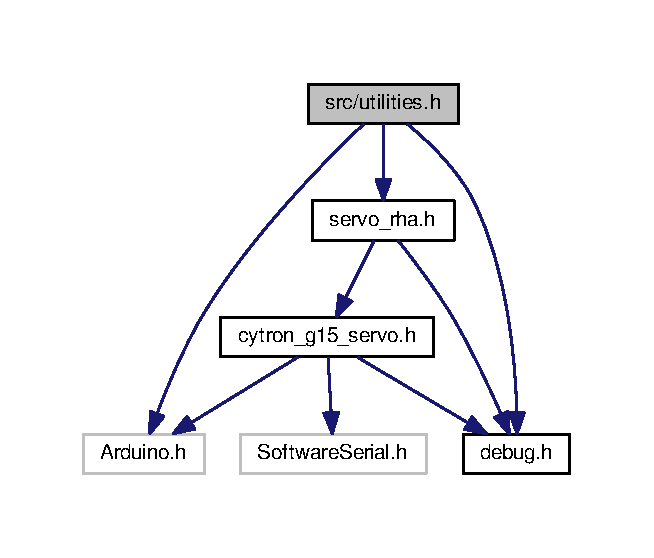
\includegraphics[width=350pt]{utilities_8h__incl}
\end{center}
\end{figure}
This graph shows which files directly or indirectly include this file\+:
\nopagebreak
\begin{figure}[H]
\begin{center}
\leavevmode
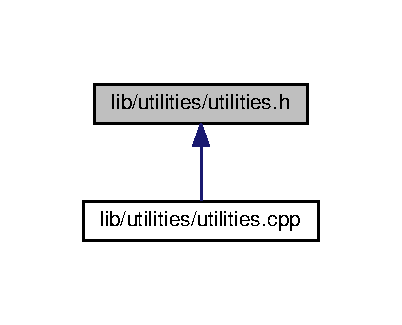
\includegraphics[width=193pt]{utilities_8h__dep__incl}
\end{center}
\end{figure}
\subsection*{Classes}
\begin{DoxyCompactItemize}
\item 
class \hyperlink{classJHUtilitiesJH}{J\+H\+Utilities\+JH}
\end{DoxyCompactItemize}
\subsection*{Macros}
\begin{DoxyCompactItemize}
\item 
\#define {\bfseries L\+ED}~13\hypertarget{utilities_8h_aeb7a7ba1ab7e0406f1b5ab36d579f585}{}\label{utilities_8h_aeb7a7ba1ab7e0406f1b5ab36d579f585}

\item 
\#define {\bfseries S\+A\+M\+P\+L\+E\+\_\+\+R\+E\+G\+U\+L\+A\+T\+OR}~500\hypertarget{utilities_8h_a23d0dd726b0c42cfeb03845129b9e7a9}{}\label{utilities_8h_a23d0dd726b0c42cfeb03845129b9e7a9}

\item 
\#define {\bfseries S\+P\+E\+E\+D\+\_\+\+R\+E\+G\+U\+L\+A\+T\+O\+R\+\_\+\+T\+E\+ST}~120\hypertarget{utilities_8h_acf96f88e55dad8de1f9026be438806e8}{}\label{utilities_8h_acf96f88e55dad8de1f9026be438806e8}

\item 
\#define {\bfseries S\+A\+M\+P\+L\+E\+\_\+\+KP}~3\hypertarget{utilities_8h_aded86b28fa3f6f2f2f90159c16b29e81}{}\label{utilities_8h_aded86b28fa3f6f2f2f90159c16b29e81}

\item 
\#define {\bfseries K\+P\+\_\+\+S\+A\+M\+P\+L\+ES}~\{2, 2, 2\};\hypertarget{utilities_8h_a05d8a7ab39f83efcb80b8d3a977aa525}{}\label{utilities_8h_a05d8a7ab39f83efcb80b8d3a977aa525}

\item 
\#define {\bfseries K\+D\+\_\+\+S\+A\+M\+P\+L\+ES}~\{0, 0.\+5, 0\};\hypertarget{utilities_8h_a41468329dd7dea43493ac68528d75b72}{}\label{utilities_8h_a41468329dd7dea43493ac68528d75b72}

\item 
\#define {\bfseries K\+I\+\_\+\+S\+A\+M\+P\+L\+ES}~\{0, 0, 0.\+1\};\hypertarget{utilities_8h_a2d1d6e4a9a80391bb0bfe5b5d094fb1d}{}\label{utilities_8h_a2d1d6e4a9a80391bb0bfe5b5d094fb1d}

\item 
\#define {\bfseries S\+T\+EP}~0\hypertarget{utilities_8h_a70be2dc5c8bdc85b027ea6118753cca1}{}\label{utilities_8h_a70be2dc5c8bdc85b027ea6118753cca1}

\item 
\#define {\bfseries S\+L\+O\+PE}~1\hypertarget{utilities_8h_a41bc3687e849cfb7c4486c66e2130ef1}{}\label{utilities_8h_a41bc3687e849cfb7c4486c66e2130ef1}

\item 
\#define {\bfseries S\+A\+M\+P\+L\+E\+\_\+\+S\+T\+EP}~300\hypertarget{utilities_8h_ab0ad7e747377ae1ac9490e5300c324ea}{}\label{utilities_8h_ab0ad7e747377ae1ac9490e5300c324ea}

\item 
\#define {\bfseries S\+A\+M\+P\+L\+E\+\_\+\+T\+E\+S\+T\+\_\+\+S\+T\+EP}~20\hypertarget{utilities_8h_affdb5c26a8a7cc9fe9a1ccf174261713}{}\label{utilities_8h_affdb5c26a8a7cc9fe9a1ccf174261713}

\item 
\#define {\bfseries S\+T\+E\+P\+\_\+\+S\+P\+E\+ED}~1023\hypertarget{utilities_8h_ad275a47ca373489fdf44ddd31e5de682}{}\label{utilities_8h_ad275a47ca373489fdf44ddd31e5de682}

\item 
\#define {\bfseries S\+A\+M\+P\+L\+E\+\_\+\+S\+L\+O\+PE}~800\hypertarget{utilities_8h_a3b803816a22dc667ea84d5bab42e9884}{}\label{utilities_8h_a3b803816a22dc667ea84d5bab42e9884}

\item 
\#define {\bfseries S\+A\+M\+P\+L\+E\+\_\+\+T\+E\+S\+T\+\_\+\+S\+L\+O\+PE}~20\hypertarget{utilities_8h_ad2f7059f2a38516ab3d9cceacda2035f}{}\label{utilities_8h_ad2f7059f2a38516ab3d9cceacda2035f}

\item 
\#define {\bfseries S\+L\+O\+P\+E\+\_\+\+S\+P\+E\+ED}~0.\+15\hypertarget{utilities_8h_ab9e892c1f3237e271d64ecb11d9822ff}{}\label{utilities_8h_ab9e892c1f3237e271d64ecb11d9822ff}

\item 
\#define {\bfseries S\+P\+E\+ED}~1023\hypertarget{utilities_8h_aac3553b3932cbfeeac4526ce7ca0336b}{}\label{utilities_8h_aac3553b3932cbfeeac4526ce7ca0336b}

\item 
\#define {\bfseries UP}~C\+CW\hypertarget{utilities_8h_a1965eaca47dbf3f87acdafc2208f04eb}{}\label{utilities_8h_a1965eaca47dbf3f87acdafc2208f04eb}

\item 
\#define {\bfseries D\+O\+WN}~CW\hypertarget{utilities_8h_a4193cd1c8c2e6ebd0e056fa2364a663f}{}\label{utilities_8h_a4193cd1c8c2e6ebd0e056fa2364a663f}

\item 
\#define {\bfseries L\+E\+D\+\_\+\+R\+O\+JO}~3\hypertarget{utilities_8h_a7885f8a39915e51a832bd4d49a003a97}{}\label{utilities_8h_a7885f8a39915e51a832bd4d49a003a97}

\item 
\#define {\bfseries L\+E\+D\+\_\+\+V\+E\+R\+DE}~4\hypertarget{utilities_8h_aa023481d2f7313e7029f4502afb8ea8d}{}\label{utilities_8h_aa023481d2f7313e7029f4502afb8ea8d}

\item 
\#define {\bfseries P\+U\+L\+S\+A\+D\+OR}~5\hypertarget{utilities_8h_a9f032eebfc4eb6466535df50d511f1b8}{}\label{utilities_8h_a9f032eebfc4eb6466535df50d511f1b8}

\end{DoxyCompactItemize}
\subsection*{Functions}
\begin{DoxyCompactItemize}
\item 
void \hyperlink{utilities_8cpp_a39f75503502cf2832b015bcba7abb43e}{Measure\+Utilities\+::average\+Chauvenet} (uint32\+\_\+t $\ast$data, uint8\+\_\+t n, float \&arithmetic\+\_\+average, float \&standard\+\_\+deviation)
\begin{DoxyCompactList}\small\item\em Calculates the average applying chauvenets criterion  average\+Chauvenet. \end{DoxyCompactList}\item 
void {\bfseries Servo\+Utilities\+::set\+Servo\+Id} (uint8\+\_\+t new\+\_\+id)\hypertarget{utilities_8h_aede02b1a7cc9de7624ff7a7d490b7f96}{}\label{utilities_8h_aede02b1a7cc9de7624ff7a7d490b7f96}

\item 
void {\bfseries Servo\+Utilities\+::full\+Factory\+Reset\+BR} ()\hypertarget{utilities_8h_aab047d18bb44eef98ff6cb81d844eac3}{}\label{utilities_8h_aab047d18bb44eef98ff6cb81d844eac3}

\end{DoxyCompactItemize}


\subsection{Detailed Description}
Implements a set of utilities to measure, experimentally, some interesting parameters. 

Measures real speed of servo, time spent with packet handling, etc

\+: Enrique Heredia Aguado $<$enheragu$>$ \+: 2017\+\_\+\+Sep\+\_\+08 \+: R\+HA \+: \hyperlink{utilities_8h}{utilities.\+h}  modified by\+: quique  modified time\+: 30-\/\+Sep-\/2017 

\subsection{Function Documentation}
\index{utilities.\+h@{utilities.\+h}!average\+Chauvenet@{average\+Chauvenet}}
\index{average\+Chauvenet@{average\+Chauvenet}!utilities.\+h@{utilities.\+h}}
\subsubsection[{\texorpdfstring{average\+Chauvenet(uint32\+\_\+t $\ast$data, uint8\+\_\+t n, float \&arithmetic\+\_\+average, float \&standard\+\_\+deviation)}{averageChauvenet(uint32_t *data, uint8_t n, float &arithmetic_average, float &standard_deviation)}}]{\setlength{\rightskip}{0pt plus 5cm}void Measure\+Utilities\+::average\+Chauvenet (
\begin{DoxyParamCaption}
\item[{uint32\+\_\+t $\ast$}]{data, }
\item[{uint8\+\_\+t}]{n, }
\item[{float \&}]{arithmetic\+\_\+average, }
\item[{float \&}]{standard\+\_\+deviation}
\end{DoxyParamCaption}
)}\hypertarget{utilities_8cpp_file_a39f75503502cf2832b015bcba7abb43e}{}\label{utilities_8cpp_file_a39f75503502cf2832b015bcba7abb43e}


Calculates the average applying chauvenets criterion  average\+Chauvenet. 


\begin{DoxyParams}{Parameters}
{\em data} & data to calculate the average \\
\hline
{\em n} & amount of data (max of 255) \\
\hline
\end{DoxyParams}
\begin{DoxyReturn}{Returns}
Returns the average 
\end{DoxyReturn}

%--- End generated contents ---

% Index
\backmatter
\newpage
\phantomsection
\clearemptydoublepage
\addcontentsline{toc}{chapter}{Index}
\printindex

\end{document}
